% ICCV 2025 Paper Template

\documentclass[10pt,twocolumn,letterpaper]{article}

%%%%%%%%% PAPER TYPE  - PLEASE UPDATE FOR FINAL VERSION
% \usepackage{iccv}              % To produce the CAMERA-READY version
% \usepackage[review]{iccv}      % To produce the REVIEW version
\usepackage[pagenumbers]{iccv} % To force page numbers, e.g. for an arXiv version
% Import additional packages in the preamble file, before hyperref
%
% --- inline annotations
%
\newcommand{\red}[1]{{\color{red}#1}}
\newcommand{\todo}[1]{{\color{red}#1}}
\newcommand{\TODO}[1]{\textbf{\color{red}[TODO: #1]}}
% --- disable by uncommenting  
% \renewcommand{\TODO}[1]{}
% \renewcommand{\todo}[1]{#1}


% It is strongly recommended to use hyperref, especially for the review version.
% hyperref with option pagebackref eases the reviewers' job.
% Please disable hyperref *only* if you encounter grave issues, 
% e.g. with the file validation for the camera-ready version.
%
% If you comment hyperref and then uncomment it, you should delete *.aux before re-running LaTeX.
% (Or just hit 'q' on the first LaTeX run, let it finish, and you should be clear).
\definecolor{iccvblue}{rgb}{0.21,0.49,0.74}
\usepackage[pagebackref,breaklinks,colorlinks,allcolors=iccvblue]{hyperref}
\usepackage{float}
\usepackage{threeparttable}
\usepackage{multicol,multirow}
\usepackage{colortbl}  %彩色表格需要加载的宏包
\usepackage{tcolorbox}
\usepackage{amsmath}  
\usepackage{algorithm}
\usepackage{algorithmic} 
\usepackage{amssymb}  
\usepackage{setspace}
\usepackage{tikz}
\usepackage{setspace}
\usepackage{pifont}
\usepackage{placeins}
\usepackage{float, afterpage}
% \usepackage{algpseudocode}
\usepackage{amsfonts}
% Add your packages here
% \usepackage{amsmath}
\newcommand{\bx}{\mathbf{x}}
\DeclareMathOperator*{\argmax}{argmax}
\usepackage{booktabs}

\usepackage{setspace}




%%%%%%%%% PAPER ID  - PLEASE UPDATE
% \def\paperID{8742} % *** Enter the Paper ID here
\def\confName{ICCV}
\def\confYear{2025}
% === 自定义脚注格式 ===
\makeatletter
% 1. 重设脚注标记为符号
\renewcommand{\thefootnote}{\fnsymbol{footnote}}
% 2. 自定义脚注显示格式
\renewcommand{\@makefntext}[1]{%
  \parindent 1em%
  \noindent%
  \hb@xt@1.8em{\hss\@makefnmark}#1%
}
\newcommand{\linebreakand}{%
  \end{@IEEEauthorhalign}
  \hfill\mbox{}\par
  \mbox{}\hfill\begin{@IEEEauthorhalign}
}

% \let\old@maketitle\@maketitle  % 保存原定义
% \renewcommand{\@maketitle}{%
%     % \vspace*{-10pt}
%   \old@maketitle  % 调用原始标题生成
%   % \vspace*{-10pt} % 在标题后统一上移
% }
\makeatother


% =============================
%%%%%%%%% TITLE - PLEASE UPDATE
% \title{Cross-Model Co-Learning for Test-Time Adaptation}
\title{When Small Guides Large: Cross-Model Co-Learning for Test-Time Adaptation}

%%%%%%%%% AUTHORS - PLEASE UPDATE
% \author{Chang'an Yi \\
% Institution1\\
% Institution1 address\\
% {\tt\small firstauthor@i1.org}
% % For a paper whose authors are all at the same institution,
% % omit the following lines up until the closing ``}''.
% % Additional authors and addresses can be added with ``\and'',
% % just like the second author.
% % To save space, use either the email address or home page, not both
% \and
% Xiaohui Deng\\
% Institution2\\
% First line of institution2 address\\
% {\tt\small secondauthor@i2.org}

% % \and
% % Guohao Chen\\
% % Institution2\\
% % First line of institution2 address\\
% % {\tt\small thirdauthor@i2.org}

% % \and
% % Shuaicheng Niu$^{\ast}$\\
% % Institution2\\
% % First line of institution2 address\\
% % {\tt\small fourthauthor@i2.org}
% }


\author{
\vspace{-10pt}
% \small % 缩小字号
\begin{tabular}{@{}c@{\hspace{1.8em}}c@{\hspace{1.8em}}c@{}}
% 第一行 (3个作者)
\parbox[t]{0.3\textwidth}{\centering
Chang'an Yi\textsuperscript{*}\\ 
Foshan University \\ 
Foshan, China \\ 
{\tt\small yi.changan@fosu.edu.cn}
} &
\parbox[t]{0.3\textwidth}{\centering
Xiaohui Deng\textsuperscript{*}\\ 
Foshan University \\ 
Foshan, China \\ 
{\tt\small 2112353032@stu.fosu.edu.cn}
} &
\parbox[t]{0.3\textwidth}{\centering
Guohao Chen\textsuperscript{*}\\ 
\makebox[\linewidth]{Nanyang Technological University} \\ 
Singapore \\ 
{\tt\small  guohao.chen@ntu.edu.sg}
} \\[10ex] % 调整行距(可选)
\parbox[t]{0.3\textwidth}{\centering
Yan Zhou\\ 
Foshan University \\ 
 Foshan, China\\ 
{\tt\small zhouyan791266@fosu.edu.cn}
} &
\parbox[t]{0.3\textwidth}{\centering
  Qinghua Lu\\ 
Foshan University \\ 
Foshan, China \\ 
{\tt\small qhlu@fosu.edu.cn}
} &
\parbox[t]{0.3\textwidth}{\centering
 Shuaicheng Niu\textsuperscript{\dag}\\ 
\makebox[\linewidth]{Nanyang Technological University} \\ 
 Singapore\\ 
{\tt\small shuaicheng.niu@ntu.edu.sg}
}
\end{tabular}
}

\begin{document}

\maketitle

% \textsuperscript{\dag}
% \textsuperscript{*}
% % 手动添加脚注内容(使用符号标记)
\footnotetext[\numexpr\value{footnote}+1]{Equal contribution. \textsuperscript{\dag}Corresponding author.}
\vspace{-100pt} 

\begin{abstract}
Test-time Adaptation (TTA) adapts a given model to testing domain data with potential domain shifts through online unsupervised learning, yielding impressive performance. However, to date, existing TTA methods primarily focus on single-model adaptation. In this work, we investigate an intriguing question: how does cross-model knowledge influence the TTA process? Our findings reveal that, in TTA's unsupervised online setting, each model can provide complementary, confident knowledge to the others, even when there are substantial differences in model size. For instance, a smaller model like MobileViT (10.6M parameters) can effectively guide a larger model like ViT-Base (86.6M parameters). In light of this, we propose COCA, a \textbf{c}ross-m\textbf{o}del \textbf{c}o-le\textbf{a}rning framework for TTA, which mainly consists of two main strategies. 1) Co-adaptation adaptively integrates complementary knowledge from other models throughout the TTA process, reducing individual model biases. 2) Self-adaptation enhances each model’s unique strengths via unsupervised learning, enabling diverse adaptation to the target domain. Extensive experiments show that COCA, which can also serve as a plug-and-play module, significantly boosts existing SOTAs, on models with various sizes—including ResNets, ViTs, and Mobile-ViTs—via cross-model co-learned TTA. For example, with Mobile-ViT's guidance, COCA raises ViT-Base's average adaptation accuracy on ImageNet-C from 51.7\% to 64.5\%. The code will be publicly available.







% Test-time Adaptation (TTA) adapts a given model to test data with potential domain shifts through online unsupervised learning, leading to impressive performance. However, existing TTA methods primarily focus on single-model adaptation, where the source domain is represented by a single model. In this work, we explore an intriguing question: how does cross-model knowledge influence the TTA process? Our findings reveal that each model can provide complementary knowledge to others, even when there are significant differences in model size. For example, a smaller model like MobileViT (10.6M parameters) can effectively guide a larger model such as ViT-Base (86.6M parameters). In light of this, we propose COCA, a \textbf{c}ross-m\textbf{o}del \textbf{c}o-le\textbf{a}rning framework for TTA. COCA consists of two main strategies, i.e., co-adaptation and self-adaptation. Co-adaptation integrates the collaborative knowledge from another model to reduce individual model biases, while self-adaptation enhances each model’s unique strengths by self-supervised learning, enabling diverse adaptation to the target domain. Extensive experiments show that COCA, as a plug-and-play module, significantly improves the performance of existing state-of-the-art methods on various models—including ResNets, ViTs, and Mobile-ViTs—through cross-model co-learned TTA. For instance, with assistance from Mobile-ViT, COCA boosts the average adaptation accuracy of ViT-Base on ImageNet-C from 51.7\% to 64.5\%. The code will be made publicly available.



% Unlike existing methods that focus on single-model adaptation, in this work, we found that different pre-trained models can provide complementary knowledge to each other. Even when one model has very low original performance, such as the significant difference between ViT-Base and ResNet-18, their collaboration can still significantly improve adaptation. This suggests that utilizing different models, rather than just one, may significantly enhance the adaptation process. To this end, we introduce COCA, a \textbf{\underline{c}}ross-m\textbf{\underline{o}}del \textbf{\underline{c}}o-le\textbf{\underline{a}}rning approach designed to improve TTA by investigating the mutual promotion across different models. In COCA, each model leverages both its knowledge and the collaborative knowledge from the other model to enhance its development, while also contributing its knowledge to enrich the shared collaborative knowledge. Our extensive experiments demonstrate that COCA effectively harnesses both the individual strengths of each model and the benefits of cross-model collaboration, leading to significant improvements in TTA performance. The source code will be publicly available.

% We found that, unlike traditional co-learning in supervised settings—where similar model scales are typically required—in the unsupervised online setting, each model can provide complementary, confident knowledge to the others, even when there is a significant size difference. For example, a smaller model like MobileViT can still guide a larger model like ViT-Base.

% In COCA, each model benefits not only from its own knowledge but also from the collaborative knowledge shared with other models, thereby enhancing its performance while contributing to the collective knowledge pool.


% Test-time Adaptation (TTA) aims to adapt knowledge from a source model to a different but related domain in an online manner. Unlike existing methods that focus on single-model adaptation, in this work, we found that different pre-trained models can provide complementary knowledge to each other. Even when one model has very low original performance, such as the significant difference between ViT-Base and ResNet-18, their collaboration can still significantly improve adaptation. This suggests that utilizing different models, rather than just one, may significantly enhance the adaptation process. In this paper, we introduce COCA, a \textbf{\underline{c}}ross-m\textbf{\underline{o}}del \textbf{\underline{c}}o-le\textbf{\underline{a}}rning approach designed to improve TTA by investigating the mutual promotion across different models. In COCA, each model leverages both its knowledge and the collaborative knowledge from the other model to enhance its development, while also contributing its knowledge to enrich the shared collaborative knowledge. Our extensive experiments demonstrate that COCA effectively harnesses both the individual strengths of each model and the benefits of cross-model collaboration, leading to significant improvements in TTA performance. The source code will be publicly available. 

% Test-Time Adaptation (TTA) aims to adapt knowledge from a source model to a new, but related, target domain in an online manner. Most existing TTA methods rely on a single model for self-supervised learning in the target domain, with techniques like entropy minimization. However, these methods often overlook the limited amount of information a single model can leverage for effective adaptation. To address this limitation, we propose a novel strategy called COCA (\textbf{\underline{c}}ross-m\textbf{\underline{o}}del \textbf{\underline{c}}o-le\textbf{\underline{a}}rning). Specifically, for each target sample, different models exhibit distinct predictive behaviors. By decomposing the models' outputs into discrepancy and consensus, we facilitate collaborative learning, allowing models to mutually enhance each other's performance. In addition, we design an adaptive integration mechanism that effectively combines the outputs of models, leading to enhanced performance. Our extensive experiments demonstrate that COCA successfully harnesses the individual strengths of each model, as well as the benefits of cross-model collaboration, resulting in significant performance improvements for TTA. The source code will be made publicly available.

\end{abstract}
   
\vspace{-0.25in}



\section{Introduction}
\label{sec:intro}

% \red{PLEASE add missing references in this section}

Deep neural networks have demonstrated remarkable performance when the training and test domains follow the same data distribution \cite{lu2022survey}. However, their accuracy drops significantly when testing data suffers from distribution shifts \cite{lu2022survey,liang2024comprehensive}.
% , which is frequently encountered in the real world~\cite{hendrycks2019benchmarking}. 
To address this, numerous attempts have been explored, such as unsupervised domain adaptation \cite{ge2023unsupervised}, source-free domain adaptation~\cite{li2024comprehensive}, and domain generalization \cite{zhou2022domain}. However, in dynamic applications like autonomous driving, environmental conditions are constantly evolving, causing continuous data distribution shifts~\cite{li2023lwsis,sakaridis2021acdc}. To maintain stable and excellent performance, models need to adapt continuously to new conditions—an especially challenging task given the unpredictability of new environments~\cite{pan2020unsupervised}.  

% However, these methods fail to perform well when the domain shift changes constantly in an unpredictable manner. 

% \red{pls use another example, simulation and real-world is too ideal} 


% \For example, each domain developed a lung diagnosis model tailored to a specific hospital using its own CT images. Although the collected images represent the same disease, the data distributions vary across domains due to differences in the CT equipment used by different hospitals. Consequently, a model may struggle to perform effectively on data from another domain because of these domain shifts. 
% Deep neural networks (DNNs) perform perfectly when the training and test domains share the same data distribution. However, the performance drops dramatically when domain shifts exist~\cite{lu2022survey,liang2024comprehensive}. A typical example of domain shifts is the gap between a simulation environment and a real scenario for the same robot~\cite{kim2022ev}. In real-world applications like autonomous driving, the perceived scenarios change continuously, leading to persistent variations in data distribution~\cite{li2023lwsis,sakaridis2021acdc}. Therefore, a computational model must constantly adapt to new conditions. This requirement is too difficult to satisfy since the new environment is unpredictable~\cite{pan2020unsupervised}. Recently, test-time adaptation (TTA) has emerged as a promising paradigm for addressing such challenges in an online manner~\cite{wang2020tent,niu2023towards,lee2024entropy,liang2024comprehensive}.


\begin{figure*}[t]
\centering
% 子图1
\begin{subfigure}[t]{0.33\textwidth} 
    \centering
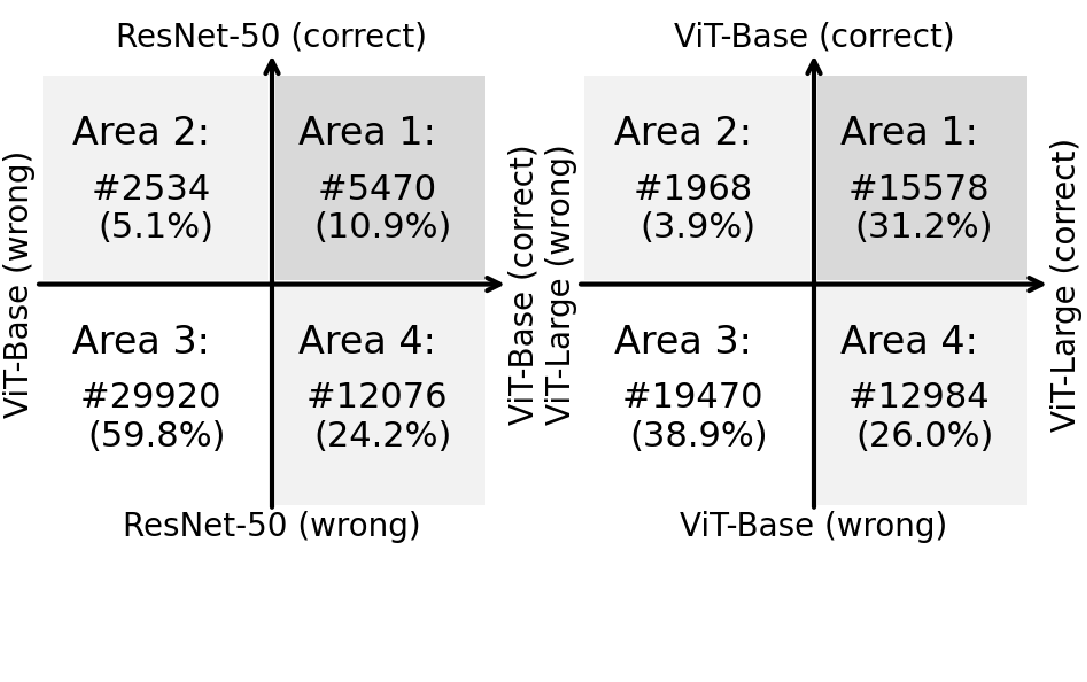
\includegraphics[width=\linewidth]{sec/fig1a_2.pdf}
\subcaption{Distinctness of model predictions
}
    \label{fig1a}
\end{subfigure}
\hfill
% 子图2
\begin{subfigure}[t]{0.34\textwidth}
    \centering
    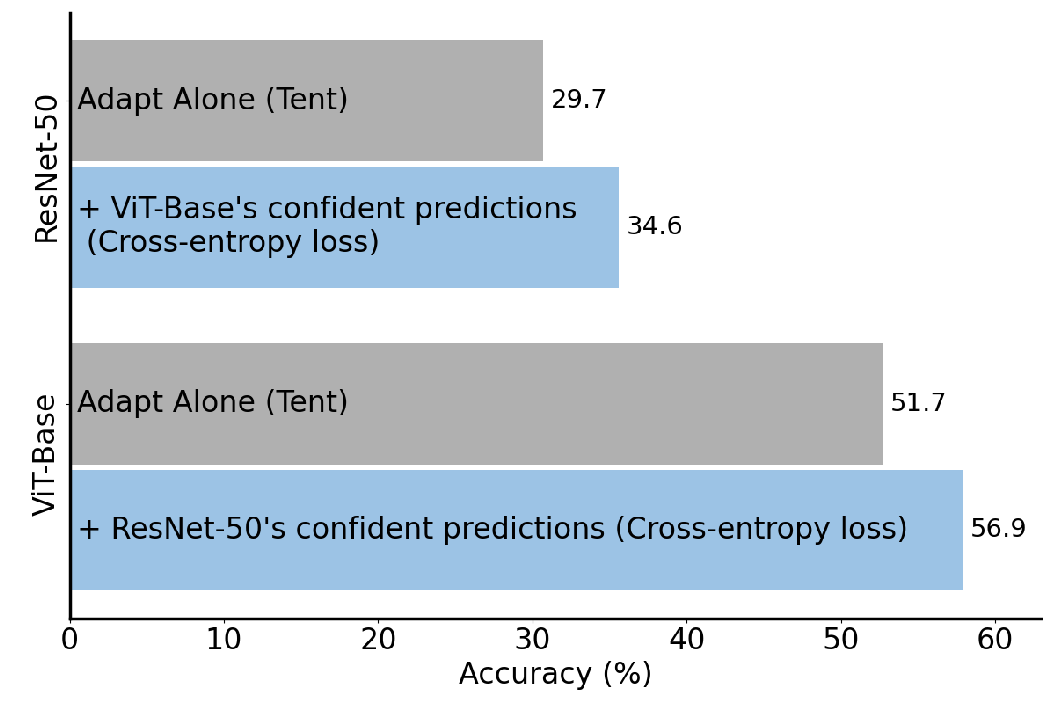
\includegraphics[width=\linewidth]{sec/fig1b_2.pdf}
    \subcaption{Benefits of complementary knowledge
}
    \label{fig1b}
\end{subfigure}
\hfill
% 子图3
\begin{subfigure}[t]{0.32\textwidth}
    \centering
    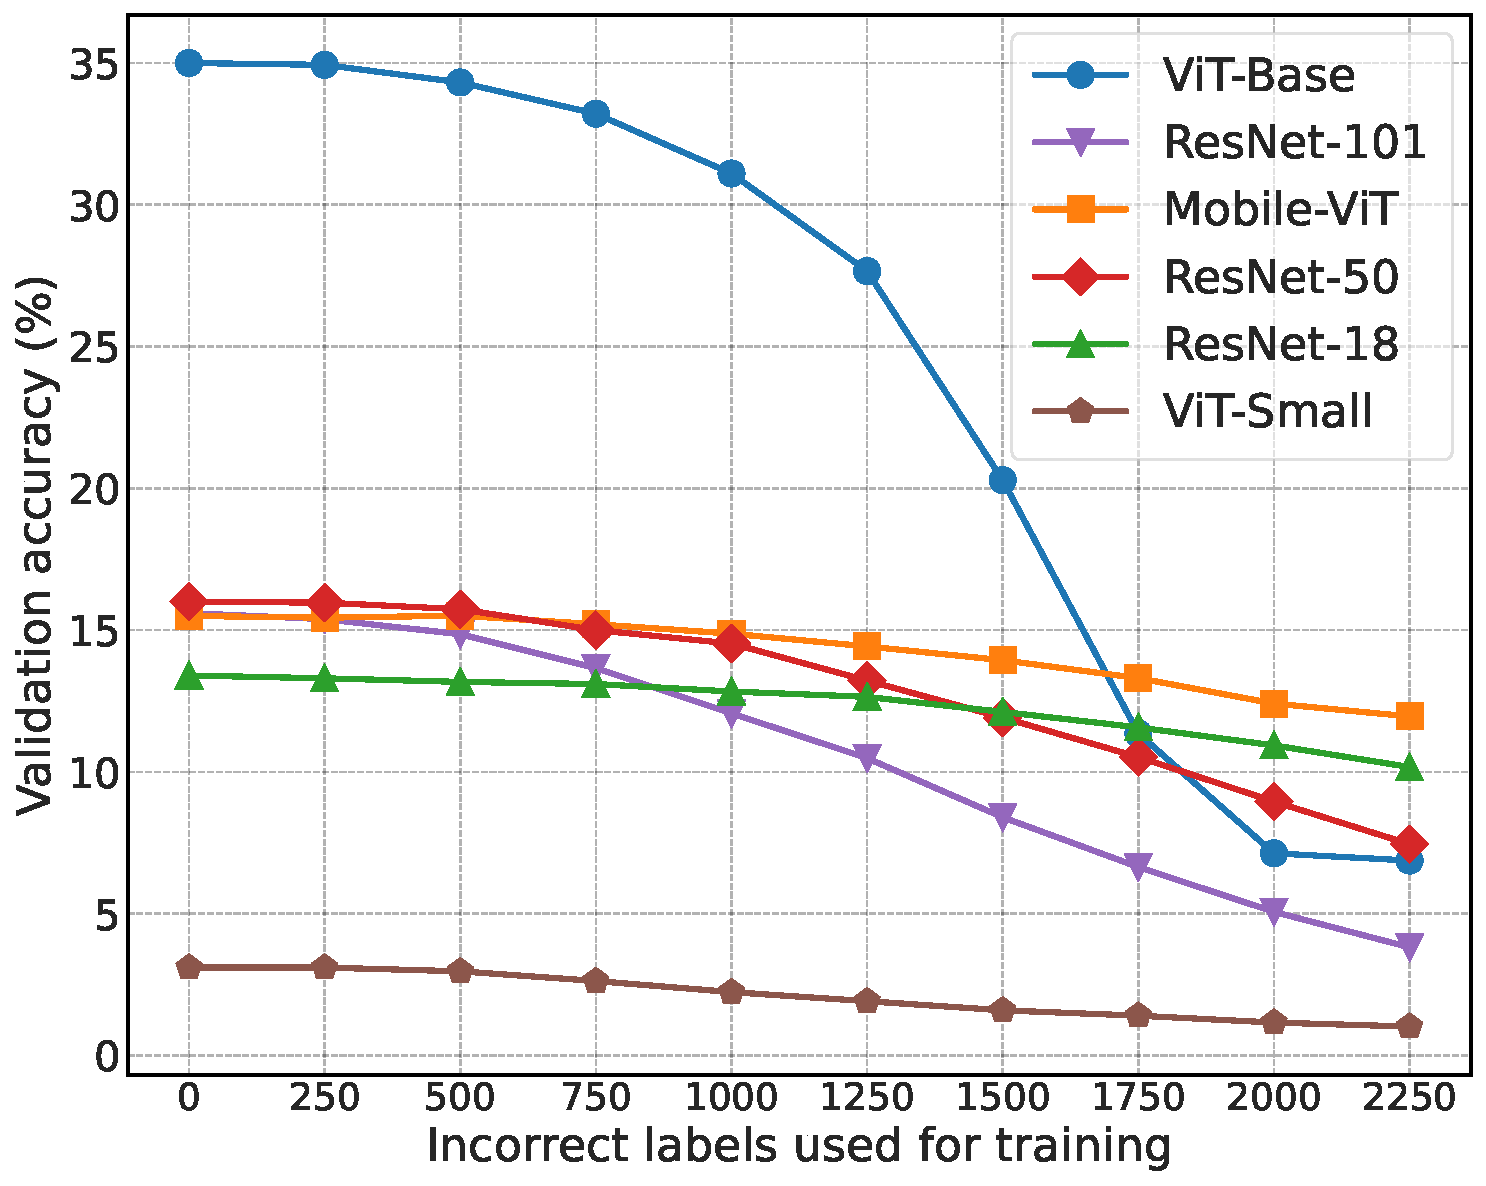
\includegraphics[width=\linewidth]{sec/fig1c_2.pdf}
    \subcaption{TTA robustness against noisy labels 
}
    \label{fig1c}
\end{subfigure}

\vspace{-0.1in}
\caption{Motivation for COCA. (a) Pre-trained models exhibit distinct strengths due to differences in training strategies, architectures, or sizes. (b) TTA~\cite{wang2020tent}, using complementary confident predictions from another model, significantly enhances adaptation performance. (c) Larger models are more vulnerable to erroneous guidance than smaller ones, highlighting differences in robustness during test time. Results are based on predicting ImageNet-C (Gaussian noise, level 5) with various ResNet-based~\cite{he2016deep} and Transformer-based~\cite{dosovitskiy2020image} models. Confident samples are filtered using an entropy threshold of 0.4*ln1000 following EATA~\cite{niu2022efficient}.}
\label{motifig1}
\vspace{-0.2in}
\end{figure*}


% \begin{figure*}[t]
%     \centering  
%     \includegraphics[width=\linewidth]{sec/fig1_3.7.pdf}
%     \vspace{-0.3in}
%     \caption{Motivation for COCA. (a) Pre-trained models exhibit distinct strengths due to differences in training strategies, architectures, and sizes. (b) TTA~\cite{wang2020tent}, using complementary confident predictions from another model, significantly enhances adaptation performance. (c) Larger models are more vulnerable to erroneous guidance than smaller ones, highlighting differences in robustness during test time. Results are based on predicting ImageNet-C (Gaussian noise, level 5) with various ResNet-based and Transformer-based models. Confident samples are filtered using a threshold of 0.4*ln1000 as defined by EATA~\cite{niu2022efficient}.}
%     \vspace{-0.15in}
%     \label{motifig1}
% \end{figure*}

% (a) Despite substantial differences in model architecture, parameter size, and TTA performance, pre-trained models always exhibit complementary knowledge and unique strengths. (b) Larger models are more susceptible to erroneous supervision, highlighting their varying robustness during test-time adaptation. (c) Motivated by these observations we introduce a simple co-learning strategy for TTA~\cite{wang2020tent}, where confident predictions from another model, filtered with a threshold of 0.4*ln1000 (as defined by EATA~\cite{niu2022efficient}), are used as pseudo-labels. This approach leads to a significant improvement in adaptation performance.




% \begin{figure}[t]
%     \centering  
%     \includegraphics[width=\linewidth]{sec/fig1.pdf}
%     \caption{Motivation of Test-Time Co-Learning. (a) Each model possesses its own confident predictions (knowledge), which are both shared with and complementary to the other. \# The number of samples is counted based on the source model. (b) TTA~\cite{wang2020tent} using complementary confident predictions from the other model is able to enhance adaptation performance a lot. Results obtained on ImageNet-C (Gaussian noise, level 5) with ViT-B (ViT-Base) and RN-50 (ResNet-50). }
%     \vspace{-0.1in}
%     \label{motifig1}
% \end{figure}
% An illustration showing the motivation of this work. (a) shows that two models produce different confident level predictions (confident and unconfident is divided by threshold 0.4*ln(1000) follow EATA~\cite{niu2022efficient} setting)for the same 50000 samples (Gauss noise of ImageNet-C). (b) demonstrates that one model can achieve significant improvement by learning from another(+ ViT-B/RN-50's knowledge denotes using its predictions as pseudo-labels for an extra cross-entropy loss).

% \red{unsupervised domain adaptation (UDA) aims to transfer models from a source domain to a target domain without access to labeled target data. This is typically achieved by learning domain-invariant feature representations \cite{li2020model, liang2020we} or through adversarial alignment \cite{liu2021adversarial}. Building upon this foundation, the fully test-time adaptation (TTA) setting was proposed \cite{wang2020tent}, where no source data or supervision is available during testing. In this setting, the model must adapt to the target domain in real-time, without revisiting the same target samples. This setup reflects the need for adaptation in practical, real-world scenarios where the target data is continuously changing and no labeled data is available.}
% \red{PLEASE introduce other works for addressing domain shifts such as unsupervised domain adaptation, domain generalization, etc., then introducing TTA: how TTA works and its advantages over prior methods, our introduction is too short}

% To achieve this, Recently, Test-time adaptation (TTA) has gained considerable attention as a promising approach for handling these shifts and challenges in real time~\cite{wang2020tent,niu2023towards,lee2024entropy,liang2024comprehensive}.

Recently, test-time adaptation (TTA) has emerged as a promising paradigm for tackling these challenges~\cite{sun2020test,liu2021ttt++,niu2023towards,lee2024entropy,liang2024comprehensive}. By directly leveraging test data through self-supervised or unsupervised objectives, TTA benefits from an online, source-free approach. This is especially true for fully TTA methods~\cite{wang2020tent,niu2022efficient}, which can be applied to any pre-trained model, thereby significantly broadening its appeal in real-world applications compared to earlier techniques. 
However, existing TTA methods~\cite{wang2020tent,niu2022efficient,lee2024entropy} typically focus on single-model adaptation and are excessively sensitive to pseudo label noise. 
Motivated by the success of co-learning~\cite{zhang2018deep} and knowledge distillation~\cite{hinton2015distilling,mirzadeh2020improved} in conventional supervised learning, we pose a natural question: Can co-learning also enhance TTA? 

To investigate this, we conduct two key experiments to examine the complementary capabilities of different models during TTA, revealing that: 1) \textit{Complementary knowledge between models}: As from Fig.~\ref{motifig1}(a), we show that different models can yield complementary predictions for the same data due to variations in training strategies, architectures, or sizes.
By leveraging the complementary confident samples from the other model to construct a pseudo cross-entropy loss during TTA, we significantly improve the adaptation performance on both the large and small model compared to Tent~\cite{wang2020tent}. 2) \textit{Differential robustness of models in TTA}: We evaluate the TTA robustness of various models by adapting them to test samples with randomly erroneous labels, using the same learning rate as in Tent~\cite{wang2020tent}. While larger models initially yield higher accuracy, they are more sensitive to incorrect pseudo labels during TTA, as shown in Fig.\ref{motifig1}(c). These findings indicate the potential of a small model to significantly improve the TTA performance and robustness of a larger model through cross-model co-learning.


% Recently, test-time adaptation (TTA) has emerged as a promising paradigm for addressing such challenges~\cite{sun2020test,liu2021ttt++,niu2023towards,lee2024entropy,liang2024comprehensive}, which directly learns from test data through self-supervised or unsupervised objectives. Benefiting from its online and unsupervised nature without access to source data, particularly of fully TTA methods~\cite{wang2020tent,niu2022efficient} that can be applied to any pre-trained model, TTA has broadened its practical appeal in real-world applications compared to prior techniques. Though effective at handling the domain shift issue, existing TTA methods~\cite{wang2020tent,niu2022efficient,lee2024entropy} typically focus on single-model adaptation. Inspired by the success of co-learning~\cite{zhang2018deep} and knowledge distillation~\cite{hinton2015distilling,mirzadeh2020improved,beyer2022knowledge} in conventional supervised learning, we ask: can co-learning also be effective for TTA in an online unsupervised setting? 

% To explore this, we first compare how different models predict identical inputs to assess their complementary knowledge. Using ResNet~\cite{he2016deep} and Transformer~\cite{dosovitskiy2020image} backbones, Fig.~\ref{motifig1}(a) shows that different models yield distinct predictions for the same data without adaptation, reflecting differences in training strategies, architectures, or sizes. Building on this observation, we leverage these complementary samples to construct a pseudo cross-entropy loss that assists the other model during TTA, using Tent~\cite{wang2020tent}. As illustrated in Fig.~\ref{motifig1}(b), incorporating complementary information from another model significantly enhances the adaptation performance of the current model. Additionally, we guide each model’s test-time adaptation using randomly erroneous labels. In each training and validation round, there is no overlap between samples. Fig.\ref{motifig1}(c) shows that larger models are more sensitive to incorrect guidance than smaller ones, indicating varying robustness during test time. These findings highlight the potential of cross-model co-learning to enhance TTA.


% (a) Despite substantial differences in model architecture, parameter size, and TTA performance, pre-trained models always exhibit complementary knowledge and unique strengths. (b) Larger models are more susceptible to erroneous supervision, highlighting their varying robustness during test-time adaptation. (c) Motivated by these observations we introduce a simple co-learning strategy for TTA~\cite{wang2020tent}, where confident predictions from another model, filtered with a threshold of 0.4*ln1000 (as defined by EATA~\cite{niu2022efficient}), are used as pseudo-labels. This approach leads to a significant improvement in adaptation performance.


In light of the above motivation, we propose a novel approach called COCA — \textbf{c}ross-m\textbf{o}del \textbf{c}o-le\textbf{a}rning for enhanced TTA, which mainly consists of two strategies, \ie, co-adaptation and self-adaptation. Co-adaptation integrates complementary knowledge between models during TTA to reduce individual biases. To achieve this, we introduce an adaptive temperature-scaled marginal entropy loss to promote mutual learning. The adaptive temperature is automatically determined via an anchor-guided alignment loss, using the larger model as an anchor. This enables robust knowledge aggregation, particularly when there is a significant size disparity between models, or the learning signals from the smaller models can otherwise be overstated or overlooked. Additionally, we propose a cross-model knowledge distillation loss, leveraging combined predictions as pseudo-labels to supervise both models and maximize the effective use of cross-model knowledge. On the other hand, self-adaptation allows each model to independently adapt using existing unsupervised learning objectives from single-model TTA, enhancing each model’s unique strengths and fostering diverse adaptation to the target domain. 
% Finally, the predictions from both adapted models can be either independently or adaptively ensembled to generate the final prediction for the test data.


% 1) Co-adaptation, which integrates the complementary knowledge between models for TTA to mitigate individual model biases; and 2) Self-adaptation, which enhances each model’s unique strengths by unsupervised learning, enabling diverse adaptation to the target domain.
% Beyond co-adaptation, the self-adaptation strategy allows each model to independently adapt within its own branch using existing single-model TTA objectives. This approach enhances each model’s unique strengths through unsupervised learning, facilitating diverse adaptation to the target domain  



% Based on co-adaptation, COCA integrates the complementary knowledge between models to mitigate individual model biases. Based on self-adaptation, COCA enhances each model’s unique strengths by unsupervised learning, enabling diverse adaptation to the target domain. Then, the predictions from both adapted models are adaptively ensembled to produce final predictions for the test data.



% In light of the above motivation, we propose a novel approach called COCA — \textbf{c}ross-m\textbf{o}del \textbf{c}o-le\textbf{a}rning for enhanced TTA, which aims to explore the mutual improvement across different models to better fit the target data. The motivation of this paper is illustrated in Fig.~\ref{motifig1}, where ViT-B, RN-50, and CE represent ViT-Base, ResNet-50, and Cross-Entropy, respectively. COCA mainly consists of two strategies, i.e., co-adaptation and self-adaptation. Based on co-adaptation, COCA integrates the complementary knowledge between models to mitigate individual model biases. Based on self-adaptation, COCA enhances each model’s unique strengths by unsupervised learning, enabling diverse adaptation to the target domain. Then, the predictions from both adapted models are adaptively ensembled to produce final predictions for the test data.


% COCA employs two main strategies: 1) Co-adaptation, which integrates the complementary knowledge between models for TTA to mitigate individual model biases; and 2) Self-adaptation, which enhances each model’s unique strengths by unsupervised learning, enabling diverse adaptation to the target domain. Then, we adaptively ensemble the predictions from both adapted models to achieve more robust predictions for the test data.

% In light of the above motivation, we propose a novel approach called COCA — \textbf{c}ross-m\textbf{o}del \textbf{c}o-le\textbf{a}rning for enhanced TTA. COCA aims to explore the mutual improvement across different models to better fit the target data. The general idea of this paper is illustrated in Fig.~\ref{motifig1}, where ViT-B and RN-50 represent ViT-Base and ResNet-50, respectively. For each model, it is evident that traditional techniques, such as entropy minimization, can enhance performance. However, leveraging the knowledge from another model can further boost the performance of each individual model. Therefore, cross-model co-learning, where knowledge is exchanged bidirectionally, holds significant promise. This paper focuses on exploring this approach and aims to provide valuable insights for the TTA community, as various models are readily available, yet the co-learning mechanism remains underexplored. \red{This paragraph needs re-writing according to the method section!!!, actually there is no description of our detailed method now.........}

A key distinction of COCA from conventional methods is its bi-directional learning capability. Unlike typical teacher-student frameworks that distill knowledge unidirectionally from a powerful teacher to a weaker student~\cite{deng2019cluster,deng2023harmonious,hu2022teacher}, or co-learning schemes where models with similar architectures are involved~\cite{wang2022continual,dobler2023robust,zhou2023adaptive}, COCA enables every model—even those with weaker performance on out-of-distribution (OOD) data—to contribute valuable insights to others. This effective exchange of complementary knowledge allows COCA to perform well in various co-TTA scenarios, such as ResNet-18+ViT-Base and Mobile-ViT+ViT-Large, as shown in Table~\ref{allmodelssup} in Appendix. Our key contributions are as follows:

% In existing methods, only one model is trained for a given domain~\cite{gao2023back,wang2020tent,lee2023towards,lee2024continual}. However, the performance of each model is limited, resulting that the guidance information from one model might not be enough for adaptation. Additionally, different models contain different knowledge and they even extract distinct information from the same data, representing that they generate diverse predictions. Therefore, it is worth exploring the potential of cross-model cooperation to improve TTA. Although the teacher-student framework can distill information from a powerful model (teacher) to a weak one (student)~\cite{deng2019cluster,deng2023harmonious,hu2022teacher}, this kind of adaptation is unidirectional where the teacher can not learn from the student and the student can not surpass the teacher. Thus, co-learning across two models might provide a new research trend for TTA. 



% In this paper, we propose a novel approach called COCA, investigating the mechanism of \textbf{\underline{c}}ross-m\textbf{\underline{o}}del \textbf{\underline{c}}o-le\textbf{\underline{a}}rning to address TTA. COCA aims to explore the mutual improvement across different models to better fit the target data. The general idea of this paper is illustrated in Fig.~\ref{motifig1}, where ViT-B and RN-50~\cite{he2016deep} represent ViT-Base and ResNet-50, respectively. For each model, it is evident that traditional techniques, such as entropy minimization, can enhance performance. However, leveraging the knowledge from another model can further boost the performance of each individual model. Therefore, cross-model co-learning, where knowledge is exchanged bidirectionally, holds significant promise. This paper focuses on exploring this approach and aims to provide valuable insights for the TTA community, as various models are readily available, yet the co-learning mechanism remains underexplored. 




\begin{itemize}

     \item We reveal that two distinct models in TTA can mutually enhance each other. Each model extracts useful information from the other's predictions, improving TTA performance and stability, even when there is a large disparity in model size, such as between Mobile-ViT (10.6M parameters) and ViT-Large (304.2M parameters). 
     
     % Furthermore, the co-adaptation between edge models like ResNet-18 and Mobile-ViT outperforms the performance of a much larger model like ResNet-101.
     
     % Even a tiny model can enhance both the performance and Expected Calibration Error (ECE) of a large model.
     
     \item We propose COCA, a novel approach that seamlessly integrates co-adaptation and self-adaptation. Co-adaptation is achieved via adaptive temperature-scaled marginal entropy loss and cross-model distillation loss, enabling knowledge sharing to reduce biases. Self-adaptation enhances each model's unique strengths via unsupervised learning, enabling diverse adaptation to target data. 
     
     \item Extensive experiments show that COCA, which is also a plug-and-play module, significantly boosts TTA performance and stability across various co-adaptation scenarios. Moreover, it introduces minimal GPU overhead, and offers a flexible performance-efficiency tradeoff by incorporating smaller models like ResNet-18.
     
     


     % \item We have conducted extensive experiments with a variety of models. The comparative results show that COCA significantly raises the performance ceiling of traditional TTA methods through mutual enhancement. Furthermore, COCA serves as a general framework that can boost the performance of existing techniques.
\end{itemize}


     % wi a cross-model co-adaptation method. In COCA, we introduce a learnable parameter that facilitates the alignment between the outputs of two models, enabling them to provide available knowledge for online adaptation.





% Deep neural networks (DNNs) perform perfectly when the training and test domains share the same data distribution. However, the performance drops dramatically when domain shifts exist~~\cite{liang2024comprehensive}. A typical example of domain shifts is the gap between a simulation environment and a real scenario for the same robot. In real-world applications like autonomous driving, the perceived scenarios change continuously, leading to persistent variations in data distribution. Therefore, a computational model must constantly adapt to new conditions. This requirement is too difficult to satisfy since the new environment is unpredictable~~\cite{pan2020unsupervised}. Recently, test-time adaptation (TTA)~~\cite{liang2024comprehensive,wang2020tent,niu2023towards} has emerged as a promising paradigm for addressing such challenges in an online manner.  \\


% Deep neural networks (DNNs) perform excellently when the training and test domains share the same data distribution~~\cite{lu2022survey}. However, their performance tends to degrade significantly in the presence of domain shifts~~\cite{liang2024comprehensive}. A common instance of such shifts is the discrepancy between a simulated environment and a real-world scenario, as seen with robots operating in both settings~\cite{lee2023tta,kim2022ev}. In practical applications like autonomous driving~\cite{sojka2023ar}, the environment is dynamic, and the perceived scenarios continuously evolve, leading to persistent variations in the data distribution. As a result, computational models must be capable of adapting to these new conditions in real time. This requirement presents a considerable challenge, as the new environment is inherently unpredictable~~\cite{pan2020unsupervised}. To address these issues, test-time adaptation (TTA)~~\cite{liang2024comprehensive,wang2020tent,niu2023towards} has emerged as a promising paradigm, offering an effective online approach to cope with domain shifts in real-world settings.\\





% Existing TTA methods focus on utilizing a single model to represent a source domain. However, the performance of each model is limited, resulting that the guidance information from this model might not be enough for adaptation. Additionally, different models contain different knowledge and they even extract distinct information from the same data, representing that they generate diverse predictions. Therefore, it is necessary to explore the potential of cross-model cooperation to improve TTA. Although the teacher-student framework~~\cite{mirzadeh2020improved,beyer2022knowledge} can distill information from a powerful model (teacher) to a weak one (student), and it has demonstrated good performance in the field of domain adaptation~~\cite{li2022cross,yang2021adversarial}, but when the scenario comes to more challenging like TTA, it is very difficult to designate a high-performance teacher to help students learn. Therefore, compared to teacher-student networks, collaborative learning that allows two models to learn from each other and surpass each other might provide a new research trend for TTA.


% Several effective TTA approaches have been proposed, which can generally be categorized into two main types, i.e., Test-Time Training (TTT)~~\cite{sun2020test, liu2021TTT++, su2022revisiting} and Fully Test Time Adaptation~~\cite{chen2022contrastive,wang2020tent}. Both types of TTA methods predominantly rely on a single model to represent the source domain and transfer knowledge to target domain. 


% However, prior TTA methods mainly only consider an individual models which means that the guidance information they provide for adaptation might be insufficient. Furthermore, different models possess distinct knowledge and may extract divergent features from the same data, leading to varying predictions. This indicates a clear need to explore cross-model collaboration to enhance TTA performance. Although the teacher-student framework~~\cite{mirzadeh2020improved,beyer2022knowledge}, which facilitates the transfer of knowledge from a more powerful model (the teacher) to a weaker one (the student), has shown promising results in domain adaptation~~\cite{li2022cross,yang2021adversarial}, applying this paradigm to the more challenging TTA scenario is fraught with difficulties. In such contexts, it is often impractical to identify a high-performance teacher model that can effectively guide student models. As a result, compared to teacher-student networks, collaborative learning—where two models learn from each other, potentially surpassing each other's individual performance—emerges as a promising alternative and could drive new advancements in TTA research.
% Recently, various large models can be freely accessed and updated to meet specific requirements. They are trained upon a huge amount of diverse data and can be tailored for different tasks. 

% In this paper, we propose a novel approach called COCA, investigating  c\textbf{\underline{r}}oss-m\textbf{\underline{o}}del \textbf{\underline{c}}o-le\textbf{\underline{a}}rning to address TTA. COCA aims to explore the mutual improvement across different models to better fit the target data. The general idea of this paper is illustrated in Fig. \ref{motifig1}, where ViT-B and RN-50 represent ViT-Base and ResNet-50, respectively. In the left of the fig, We can see that different models exhibit different prediction distributions on the same 50000 samples. By utilizing the ViT-Base correctly  predict samples, ResNet50 demonstrated significant performance improvements. At the same time, ViT-Base can also significantly improve performance by utilizing only the parts correctly predicted by ResNet-50 although this part only accounts for 5.1\% of the samples.

% However, a well-trained source model is constrained to its architecture, representing the architecture plays an important role in training the model. Therefore, it would be promising to investigate the mutual learning strategies to promote TTA across models with different architectures. The teacher-student model focuses solely on transferring knowledge from the teacher model to the student model, without any recipCOCAl transfer of knowledge from the student model back to the teacher model.



% \begin{enumerate}
%      \item To the best of our knowledge, we are the first to uncover and utilize that distinct models can interactively develop each other in a bidirectional manner. 
     
%      % Even a tiny model can enhance both the performance and Expected Calibration Error (ECE) of a large model.
     
%      \item We propose COCA, a cross-model co-learning method designed to address test-time adaptation (TTA). COCA not only serves as a standalone method but also as a flexible framework that can be integrated with traditional TTA approaches. By combining each model's individual knowledge with collaborative knowledge, COCA enhances the performance of both models and generates integrated outputs that outperform any single model, thanks to an effective output integration mechanism.

%      \item We have conducted extensive experiments with various models, and the comparative results clearly demonstrate that COCA significantly boosts TTA performance through cross-model co-learning. Moreover, COCA also can serves as a general framework that can be applied to enhance the performance of existing techniques.
% \end{enumerate}

\vspace{-0.11in}
\section{Related Works}
\vspace{-0.03in}
% The related literature of this work can be categorized into two main areas: test-time adaptation (TTA) and co-learning.

\paragraph{Test-Time Adaptation} The goal of Test-Time Adaptation (TTA) is to leverage pre-trained models and adapt them to OOD data through fine-tuning, achieving robust performance in the target domain~\cite{liang2024comprehensive}. Recently, various methods have been proposed to tackle TTA. TEA~\cite{yuan2024tea} transforms the source model into an energy-based classifier to mitigate domain shifts. AdaContrast~\cite{chen2022contrastive} combines contrastive learning and pseudo-labeling to address TTA. DomainAdapter~\cite{zhang2023domain} adaptively merges training and test statistics within normalization layers. AdaNPC~\cite{zhang2023adanpc} is a parameter-free TTA approach based on a K-Nearest Neighbor (KNN) classifier, using a voting mechanism to assign labels based on $k$ nearest samples from memory. In contrast to traditional approaches, CTTA-VDP ~\cite{gan2023decorate} introduces a homeostasis-based prompt adaptation strategy, freezing the source model parameters during continual TTA. Additionally, FOA~\cite{niu2024test} devise a fitness function that measures test-training statistic discrepancy and model prediction entropy. 
% TTAB \cite{zhao2023pitfalls} unveils three common pitfalls in prior TTA approaches under classification tasks, based on a large-scale open-sourced benchmark and thorough quantitative analysis.

Among the various TTA methods, entropy minimization has emerged as a prominent approach. For example, Tent~\cite{wang2020tent} minimizes the entropy of the model’s predictions on OOD data, adapting only the normalization layer parameters. Inspired by Tent, methods such as EATA~\cite{niu2022efficient}, MEMO~\cite{zhang2022memo}, SAR~\cite{niu2023towards}, DeYO~\cite{lee2024entropy}, and ROID~\cite{marsden2024universal2} have demonstrated strong performance in entropy-based TTA. However, most prior works leverage only the limited knowledge from a pre-trained model and thus result in constrained TTA efficacy, as shown in Table~\ref{mainres}.

% However, most prior works focus on training a single model for each source domain. 


% In contrast, our proposed method, COCA, emphasizes enabling two networks—originating from the same source domain but with different configurations—to collaborate during adaptation. This collaborative approach yields superior performance, as the combined models achieve better results than any individual model alone.
\vspace{-15pt}
\paragraph{Co-Learning} Traditional co-learning paradigms include the teacher-student framework~\cite{hu2022teacher, beyer2022knowledge}, multi-modal settings~\cite{yin2023crossmatch}, and ensemble learning~\cite{yang2023survey}. In the teacher-student setting, knowledge is transferred unidirectionally from a stronger teacher to a weaker student. In contrast, COCA operates bidirectionally, enhancing overall performance by mutually improving both models. A key distinction between COCA and multi-modal settings is that in COCA, all models share the same input and task. In typical ensemble learning, models make independent predictions that are later aggregated. However, COCA enables direct inter-model influence throughout the entire adaptation process, fostering deeper collaboration. 

In the field of domain adaptation which is related to TTA, CMT~\cite{cao2023contrastive} proposes contrastive mean teacher to maximize beneficial learning signals. Harmonious Teacher~\cite{deng2023harmonious} is a sample reweighing strategy based on the consistency of classification. TTA methods like CoTTA~\cite{wang2022continual}, RoTTA~\cite{yuan2023robust}, and RMT~\cite{dobler2023robust} have successfully applied the teacher-student paradigm within the same model, yielding strong performance. In unsupervised domain adaptation, a closely related approach is AML~\cite{zhou2023adaptive}, which tackles this issue by adaptively switching the roles of the teacher and student, thereby alleviating the challenge of selecting a powerful teacher model. However, in TTA context, determining when to switch these roles becomes more complex, primarily due to the inconsistency in confidence levels between the outputs of different models. This inconsistency makes it difficult to establish a clear criterion for role-switching.


% However, a key challenge in implementing a teacher-student architecture with different models in TTA is the difficulty of pre-defining a reliable and effective teacher model, as is typically done in traditional teacher-student networks.

% Our proposed COCA differs from existing co-learning methods by emphasizing collaborative improvement between models throughout the entire adaptation process. Unlike the traditional teacher-student framework~\cite{hu2022teacher, beyer2022knowledge}, where knowledge is transferred solely from a stronger teacher to a weaker student, COCA operates bidirectionally, enhancing overall performance by mutually improving both models. The key distinction between COCA and multi-modal~\cite{yin2023crossmatch} settings is that, in COCA, all models share the same input and task. In contrast to ensemble learning~\cite{yang2023survey}, where models typically make independent predictions that are later aggregated, COCA enables direct inter-model influence throughout the entire adaptation process, promoting deeper collaboration and dynamic knowledge exchange. By extending the performance boundaries of each model, COCA aims to achieve more effective real-time adaptation. The robustness of COCA is further ensured by the collaborative integration of the distinct advantages offered by different models.

% Our proposed COCA differs from existing TTA methods by emphasizing collaborative improvement between models. Unlike the traditional teacher-student framework~\cite{hu2022teacher, beyer2022knowledge}, where knowledge is transferred solely from a stronger teacher to a weaker student, COCA operates in a bidirectional manner, aiming to enhance overall performance while mutually improving both models. The robustness of COCA is ensured by the collaborative integration of the distinct advantages offered by different models. The key distinction between COCA and multi-modal~\cite{yin2023crossmatch} settings is that, in COCA, all models share the same input and task. In contrast to ensemble learning~\cite{yang2023survey}, where models typically make independent predictions that are later aggregated, COCA enables direct inter-model influence throughout the adaptation process, promoting deeper collaboration and dynamic knowledge exchange. By extending the performance boundaries of each model, we aim to achieve more effective real-time adaptation.

% \red{Overall performance?}
\vspace{-0.1in}
\section{Proposed Method}
\label{sec:Method Section}
\paragraph{Problem Statement} 
Let $\mathcal{D}^{train} = \{\left(\textbf{x}_i, \textbf{y}_i \right)\}_{i=1}^{N} \in \mathcal{P}^{train}$ denote the labeled training data from the source domain, where $\mathbf{x}$, $\mathbf{y}$ and $N$ represent the features, labels and data
amount, respectively. We consider two pre-trained source models, $f_{\theta_1}: \mathbf{x} \rightarrow \mathbf{y}$ and $f_{\theta_2}: \mathbf{x} \rightarrow \mathbf{y}$, parameterized by $\theta_1$ and $\theta_2$, respectively. These two models are well-trained on $\mathcal{D}^{\text{train}}$, and our goal is to adapt them to unlabeled, OOD target data in an online unsupervised manner. 

\vspace{-12pt}
\paragraph{Motivation} To fully exploit the potential of $f_{\theta_1}$ and $f_{\theta_2}$, a natural question arises: \textit{How do they benefit each other throughout the test-time adaptation process?} Unlike traditional paradigms such as the teacher-student framework~\cite{hu2022teacher}, ensemble learning~\cite{yang2023survey}, and multi-modal learning~\cite{yin2023crossmatch}, we aim to enable the models to mutually enhance each other in a bidirectional manner throughout the entire adaptation process. Additionally, the models share the same input and are designed for the same task. As shown in Fig.\ref{motifig1}, different models capture distinct facets of source knowledge due to variations in training strategies, architectures, or sizes—with larger models generally being more powerful. More importantly, Fig.\ref{motifig1} also reveals two key insights: 

\begin{itemize}

     \item \textbf{Different models offer complementary knowledge from training}.
     % In particular, these pre-trained models, even differing in sizes, can enhance one another by leveraging their respective confident predictions. 
     Though pre-trained models differ in sizes, they provide complementary confident knowledge to each other, which substantially enhances TTA performance. Taking ResNet-50 and ViT-Base as two peer collaborators, by harnessing the complementary knowledge from each other, the performance of ResNet-50 improves from 29.7\% to 34.6\%, while the performance of ViT-Base rises from 51.7\% to 56.9\% on ImageNet-C. 
     \item \textbf{Different models exhibit varying levels of robustness during TTA}. 
     % Smaller models often prove more resistant to misleading signals, which are inevitable and unpredictable in complex environments.
     While larger models are more accurate, smaller models can be more resistant to noisy learning signals, which commonly arise in complex TTA scenarios. 
     % In fact, when the adaptation process is misled by 2,250 incorrect labels, the performance of ViT-Base drops to a level comparable to that of ResNet-50.
     For example, when TTA is performed on 2,000 samples with incorrect pseudo labels, the performance of ViT-Base falls to a level even lower than that of ResNet-50.
\end{itemize}
% These observations highlight the promise of exploring cooperative adaptation mechanisms, although enabling stable co-adaptation between models of different sizes remains challenging due to the large gap of their outputs.
These observations underscore the potential of exploring cooperative TTA mechanisms. However, achieving stable co-adaptation between models of different sizes remains challenging, due to the substantial disparity in their outputs.


% vitb drop 28.1
% mobile drop 3.5
% 18 drop 3.2
% 50 drop 8.5
% 101 drop 11.7
% vits drop 2.1


% \paragraph{Motivation} Inspired from Fig.~\ref{motifig1}, different models capture different facets of source domain knowledge due to variations in training strategies, model architectures, or sizes. Notably, larger models tend to be more powerful. Despite these variations, two models can enhance one another by leveraging their complementary confident predictions. Moreover, their robustness varies when encountering erroneous information at test time, with smaller models generally being more resilient to incorrect guidance. This suggests that exploring cooperative mechanisms between different models throughout the adaptation process is promising. However, enabling effective co-adaptation between models of different sizes is challenging, as their outputs cannot be directly aligned.

% Therefore, our objective is to continuously adapt the two pre-trained source models to effectively handle each batch of target samples by leveraging cross-model co-learning. In this process, the two models complement each other, ultimately improving overall performance.
%After obtaining two pre trained models, due to the huge differences in parameter quantity, structure, and performance between the models, how to effectively utilize the knowledge of each model and enable them to collaborate? Meanwhile, since TTA focuses on the performance of the final model in the target domain, how can strong performance be demonstrated in the target domain after two models collaborate?
% In the context of test-time adaptation (TTA), a batch of unlabeled test samples arrives sequentially at each time step and is processed online without storage.
% \mathcal{X} \mathcal{Y}

% where two different source models $f_{\theta_1}\left(\textbf{x}\right)$ and $f_{\theta_2}\left(\textbf{x}\right)$ are utilized to represent the knowledge of the same domain. These two models mutually promote each other while they are simultaneously combined to better produce final predictions.
% To address this challenge, we propose a cross-model co-learning approach for TTA. Specifically, the two models $f_{\theta_1}$ and $f_{\theta_2}$ engage in mutual collaboration during adaptation. At each time step, the models share adaptation cues and insights derived from the unlabeled test data, enabling bidirectional knowledge exchange. This interaction allows each model to leverage the complementary strengths of the other, enhancing their ability to adjust to the distributional shifts between $\mathcal{P}^{\text{train}}$ and $\mathcal{P}^{\text{test}}$. Ultimately, we combine the adapted models to produce improved predictions on the test data. By integrating the strengths of both models through cross-model co-learning, our approach aims to achieve superior performance compared to traditional single-model TTA methods.

\begin{figure}[t]
\centering
    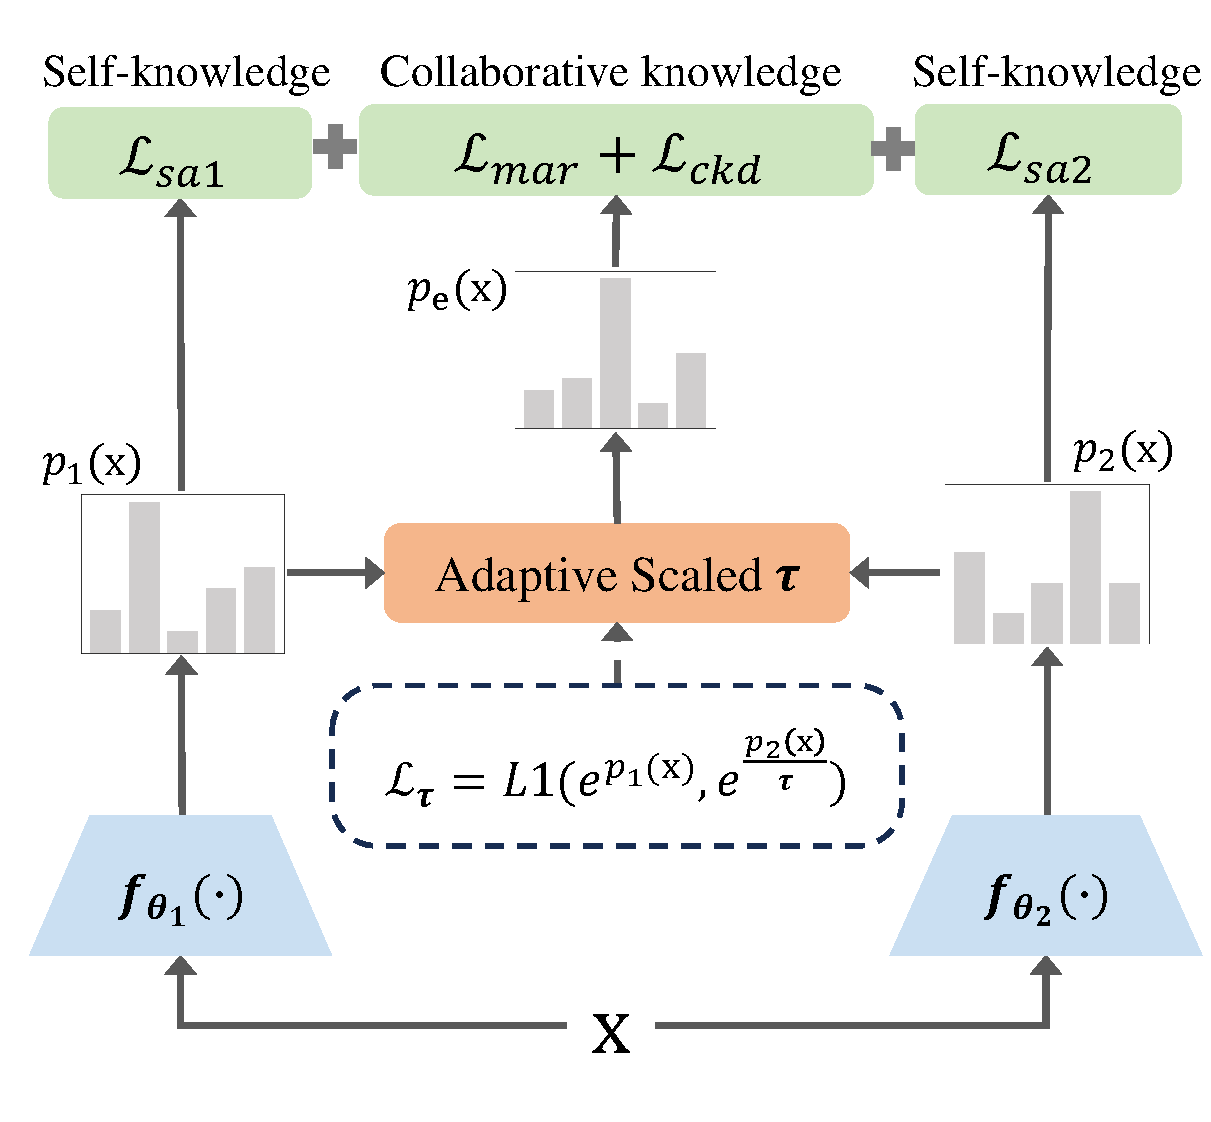
\includegraphics[width=0.93\linewidth]{sec/overview_3.7.pdf}
    % \vspace{-0.05in}
    \caption{The overall COCA framework consists of two models that adapt by leveraging both their inherent self-knowledge and the adaptive collaborative knowledge shared between them. To facilitate a more effective and robust ensemble of their outputs—namely, $p_1(\bx)$ and $p_2(\bx)$—a learnable parameter, $\tau$, is introduced. In this example, we designate $f_{\theta_2}$ as the auxiliary model, and its output is divided by $\tau$ to enable co-learning.}
    % A learnable parameter, $\tau$, is introduced to more effectively ensemble the outputs of the two models. The final predictions, $p_{com}(x)$, are derived from the combined outputs of both models.
    \vspace{-0.15in}
\label{overview}
\end{figure}


% The overall framework of COCA. Each model adapts by leveraging both its own self-knowledge and the adaptive collaborative knowledge shared with the other model. A learnable parameter, $\tau$, is introduced to enable a more effective and robust ensemble of the models' outputs, i.e., $p_1(\bx)$ and $p_2(\bx)$. In this example, we use $p_2(\bx)$ to represent the auxiliary model and the output of $p_2(\bx)$ will be divided by $\tau$.


\vspace{-11pt}\paragraph{Overall Framework} To leverage the unique strengths of different pre-trained models and address their varying robustness during test-time adaptation (TTA), we propose COCA, a cross-model co-learning approach that emphasizes an adaptive bidirectional cooperation mechanism. COCA employs two key strategies: co-adaptation and self-adaptation. The co-adaptation strategy harnesses the collaborative knowledge between models to mitigate individual biases during TTA, with adaptive alignment of outputs from models of different sizes further enhancing robustness. In contrast, the self-adaptation strategy refines each model’s unique strengths through unsupervised learning, enabling diverse and flexible adaptation to the target domain. An overview of COCA is shown in Fig.~\ref{overview}, and the corresponding pseudo-code is provided in Appendix~\ref{pscode}.

% \paragraph{Differences with Existing Paradigms}
% Our proposed COCA differs from existing TTA methods by emphasizing collaborative improvement between models. Unlike the traditional teacher-student framework~\cite{hu2022teacher, beyer2022knowledge}, where knowledge is transferred solely from a stronger teacher to a weaker student, COCA operates in a bidirectional manner, aiming to enhance overall performance while mutually improving both models. The robustness of COCA is ensured by the collaborative integration of the distinct advantages offered by different models. The key distinction between COCA and multi-modal~\cite{yin2023crossmatch} settings is that, in COCA, all models share the same input and task. In contrast to ensemble learning~\cite{yang2023survey}, where models typically make independent predictions that are later aggregated, COCA enables direct inter-model influence throughout the adaptation process, promoting deeper collaboration and dynamic knowledge exchange. By extending the performance boundaries of each model, we aim to achieve more effective real-time adaptation.

% \paragraph{Overall Framework} To exploit the diverse strengths of different pretrained models, we propose COCA, a cross-model co-learning approach for test-time adaptation (TTA). The overall details of COCA are illustrated in Fig. \ref{overview}. The key idea of our co-learning mechanism includes two strategies: i) exploiting model-specific knowledge through self-supervised learning, and ii) investigating collaborative information to further enhance each model. Predictions from both adapted models are adaptively aggregated to gain the final performance on the target domain.



% \begin{equation}\label{eq3}
% \begin{aligned}
%     \mathcal{L}_{se}=\min_{\theta}{\sum E(x)\over{\sum_{\mathbb{I}_{\{E(x; \theta)<E_0\}}x}}}.
% \end{aligned}
% \end{equation}

% The necessity of introducing the adaptive scaled temperature $\tau$. \emph{Average} refers to directly combining the outputs of the two models by averaging them to form collaborative knowledge.
\begin{figure*}[t]
\centering
    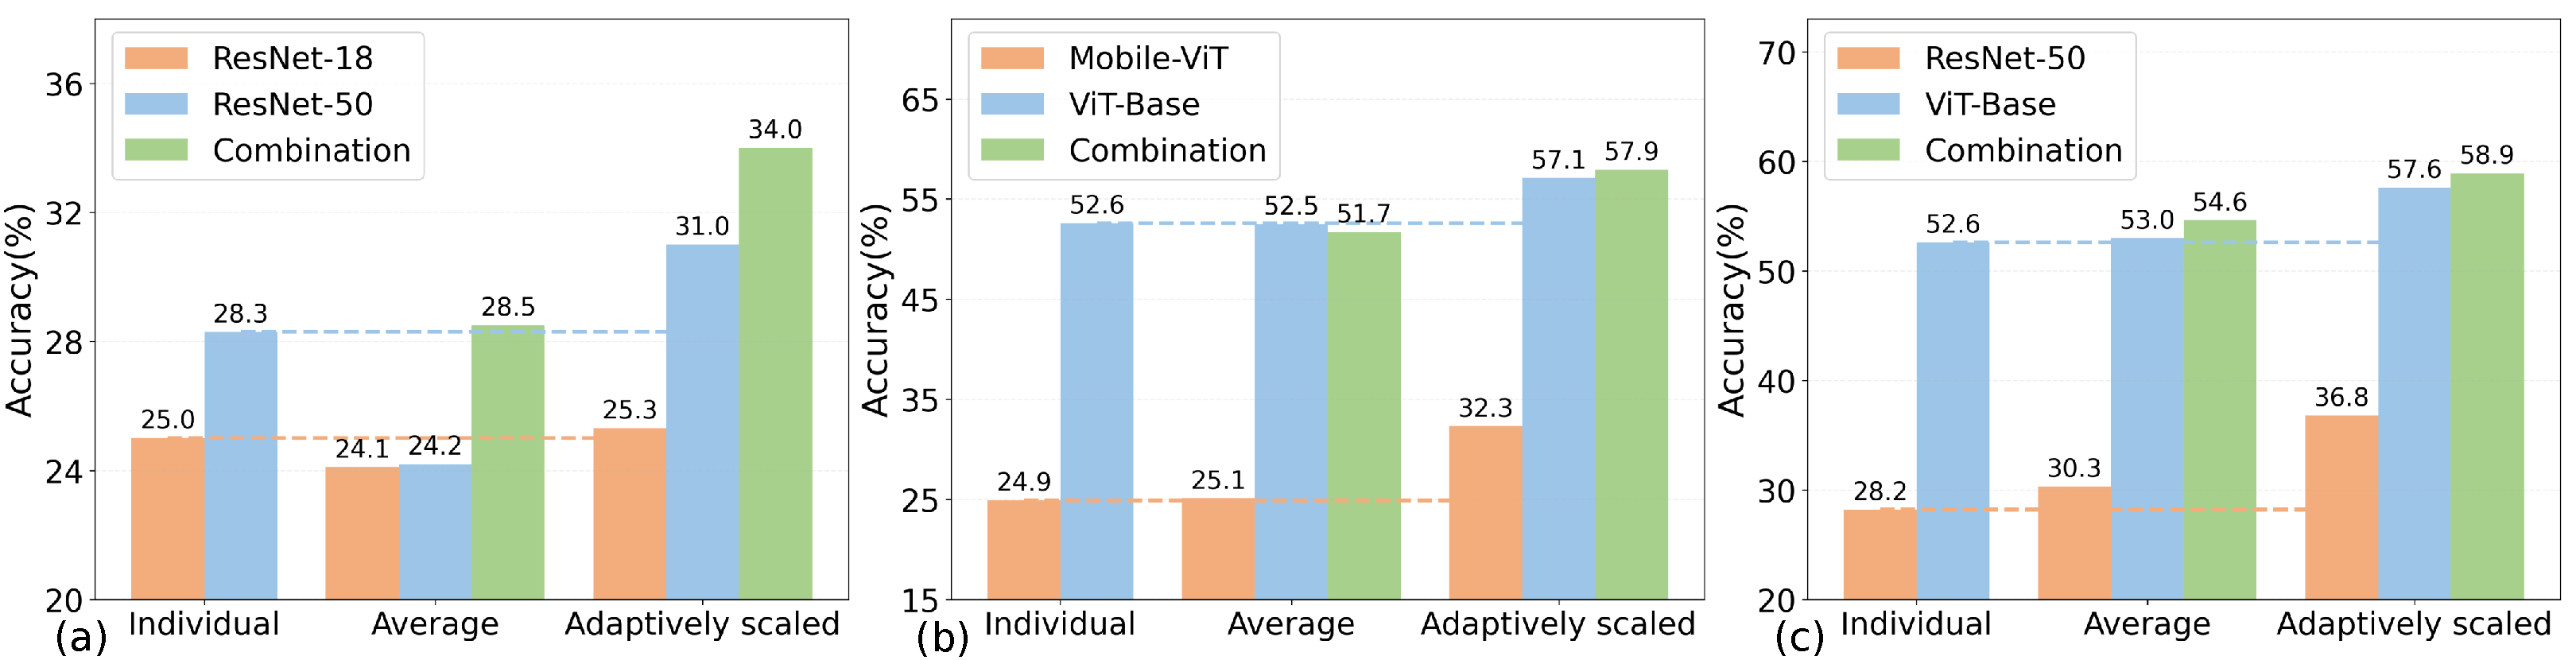
\includegraphics[width=\linewidth]{sec/Tcompare.pdf}
    \vspace{-0.25in}
    \caption{The necessity of introducing $\tau$, a learnable parameter. All experiments are based on Tent~\cite{wang2020tent}. \textit{Individual} refers to adapting each model independently, as done in Tent. \textit{Average} involves combining the predictions of two models by averaging their output logits for marginal entropy minimization. Under this strategy, the performance improvement is limited. In contrast, \textit{Adaptively scaled} utilizes the parameter $\tau$ to adaptively combine the output logits, resulting in a substantial increase in overall performance. }
    \vspace{-0.1in}
\label{Tcompare}
\end{figure*}


\subsection{Cross-Model Collaborative Adaptation} 
\label{aoi}
\label{tintro}
% overfitting
% We design COCA to integrate the complementary strengths from different models for test-time adaptation. This is important. This is challenging.
Unlike traditional TTA methods that depend solely on the limited knowledge of a single pre-trained model, our approach focuses on enhancing TTA performance and stability through cross-model collaboration. This collaborative strategy is particularly vital in the context of online unsupervised adaptation, where individual models are prone to overfitting their inherent biases and accumulating errors, as demonstrated in Table~\ref{mainres}. 

% Furthermore, we must consider two key factors, i.e., different models offer complementary knowledge from training, and different models exhibit varying levels of robustness during testing.
% To address that, our co-adaptation strategy focuses on aggregating the complementary knowledge from different models to enhance TTA. 
However, co-learning between models during testing presents significant challenges, due to both 1) varying degrees of miscalibration~\cite{naeini2015obtaining, tomani2021post} and 2) notable performance gaps in model predictions when handling OOD data. Consequently, simply averaging the outputs of multiple models for TTA can degrade overall performance, as in Fig.~\ref{Tcompare}.

% for knowledge aggregation
To make co-learning feasible at testing, we introduce a learnable diversity-aware scaling factor, $\tau$, which facilitates robust knowledge aggregation between large and small models for TTA. Specifically, in COCA, we identify the model with the larger parameter size as the \textit{anchor model}, and the other as the \textit{auxiliary model}, where larger models typically exhibit better in-distribution and out-of-distribution generalization~\cite{kim2023reliable}. 
During testing, we measure the discrepancies between the anchor predictions and the auxiliary predictions, which informs how trustworthy the auxiliary predictions are to determine the value of $\tau$. Formally, given anchor predictions logits $p_{a}(\bx)$ and auxiliary predictions logits $p_{s}(\bx)$, our goal is to learn a scaling factor $\tau$ in a unidirectional manner, so that:

\begin{equation}
    \arg \min_{\tau} \mathcal{L}_{s}(p_{a}(\bx), \frac{p_{s}(\bx)}{\tau}),
    \label{tloss}
\end{equation}
where $\mathcal{L}_{s}$ is a discrepancy function. Here, we adopt L1 loss to estimate this discrepancy, while projecting the prediction logits to the exponential space for discrepancy calculation, inspired by softmax. Then, $\mathcal{L}_{s}$ is formulated by:

\begin{equation}
    \mathcal{L}_{s}(p_a(\bx), p_s(\bx)) = \left |\left|e^{p_{a}(\bx)} - e^{p_{s}(\bx)} \right|\right|_1.
\end{equation}

We use this discrepancy loss to optimize \textit{only} the learnable factor $\tau$, and subsequently leverage $\tau$ for prediction aggregation, with the overall prediction $p_{e}(\bx)$ given by:
\begin{equation}
    p_{e}(\bx) = \frac{p_{e}'(\bx)}{T},~~\text{where}~p_{e}'(\bx)=p_{a}(\bx) + \frac{p_{s}(\bx)}{\tau}.
    \label{tau_ensemble}
\end{equation}
The learnable parameter $\tau$ serves to align the outputs of models with different sizes, thereby ensuring a more effective and robust adaptation process. The ensemble prediction is then utilized for marginal entropy minimization. Here, we introduce an adaptive balance factor $T$, defined as $\max p_{e}'(\bx) / \max p_{a}(\bx)$, to keep the max predictive logit unchanged after aggregation, maintaining a reasonable sharpness of $p_{e}(\bx)$.
Notably, the scaling factor $\tau$ does not modify the results of $p_{s}(\bx)$ but controls its contribution to the ensemble prediction $p_e(\bx)$ according to its reliability. \linebreak Experiments in Fig.~\ref{Tcompare} demonstrate the effectiveness of our $\tau$ to facilitate co-learning among models of various architectures and with different performance gaps.

% that adaptively integrates knowledge from different models
Based on the ensemble prediction $p_{e}(\bx)$, we construct the cross-model co-adaptation objective of COCA as:
\begin{equation}
\label{colloss}
    \mathcal{L}_{col} = \mathcal{L}_{mar} + \mathcal{L}_{ckd},
\end{equation}
with $\mathcal{L}_{mar}$ to enhance the separability of data in the ensemble prediction $p_e(\bx)$  and $\mathcal{L}_{ckd}$ to improve each model through knowledge distillation. We depict them below.
% We describe these components in more detail below. 
% with $\mathcal{L}_{mar}$ to enhance the separability of data in the ensemble prediction $p_e(\bx)$  and $\mathcal{L}_{ckd}$ to distill the integrated knowledge into each model. We depict them below.

\vspace{-5pt}\paragraph{Marginal Entropy Minimization} To improve the generalization of $p_e(\bx)$, our goal is to enhance the predictive confidence of $p_e(\bx)$, thereby learning a decision boundary that lies in the low-density sample region~\cite{grandvalet2004semi}. Following Tent~\cite{wang2020tent}, we adopt the entropy objective and apply it to $p_e(\bx)$ for marginal entropy minimization, defined as:
\begin{equation}
    \mathcal{L}_{mar} = - \sum_{c=1}^C p_{e}^c(\bx)\log p_{e}^c(\bx),
    \label{marginalent}
\end{equation}
where $C$ represents the number of categories.
% thereby learning a decision boundary that lies in the low-density region of the sample distribution

\vspace{-10pt}\paragraph{Cross-Model Knowledge Distillation}
In addition to $\mathcal{L}_{mar}$ that enhances the overall prediction performance, we also introduce a knowledge distillation loss to provide more direct learning signals, transferring knowledge from $p_{e}(\bx)$ to each individual model. This maximizes the utilization of cross-model knowledge in $p_e(\bx)$, and improves the generalization of each model. Specifically, we derive pseudo-labels from $p_e(\bx)$ and compute a cross-model knowledge distillation loss for each model based on cross-entropy loss: 
\begin{align}
\label{ckdloss}
\mathcal{L}_{ckd} = \mathcal{L}_{CE}(p_a(\bx),\hat{y}) + \mathcal{L}_{CE}(p_s(\bx),\hat{y}),
\end{align}
where $\hat{y}= \argmax p_e(\bx)$ denotes the pseudo-label of the ensemble prediction $p_e(\bx)$.
% to enhance the generalization of each model with more direct guidance signals
% We enhance the generalization of each model, by conducting knowledge distillation from $p_{e}(\bx)$ to the individual outputs. This xx , and thus enable a more robust TTA.
% distilling the ensemble knowledge for 

% To facilitate the flow of knowledge from the ensemble predictions to the individual models, we introduce pseudo-labels derived from the ensemble prediction $p_e(\bx)$. Using these pseudo-labels, we compute a Cross-Model Knowledge Distillation loss for each model, based on Cross-Entropy Loss:



% In the context of model co-learning, the asymmetric nature of different model architectures results in varying capacities for knowledge representation and adaptation. Generally, models with a larger number of parameters exhibit greater representational power and enhanced adaptation capabilities. When fostering collaboration among models, it is crucial to account for these differences in model capacity and adaptation potential. Motivated by this insight, we introduce the concept of an \textbf{anchor model} to establish a hierarchical collaboration framework. 

% Specifically, given two models: anchor model $f_{\theta_1}$ and non-anchor model $f_{\theta_2}$, we designate the model with more parameters as the anchor model, which serves as the primary guide during the test-time adaptation process. This design choice is founded on the intuition that the anchor model's broader knowledge base can provide more reliable adaptation directions.

% To facilitate effective knowledge transfer while preserving the complementary strengths of both models, we introduce an adaptive temperature scaling mechanism for the non-anchor model. Let $\tau$ be a learnable parameter that modulates the contribution of the non-anchor model without altering its fundamental predictions. The temperature scaling is applied as:

% \begin{equation}
% \tilde{p_2}(x) = \frac{p_2(x)}{\tau},
% \end{equation}
% where $p_2(x)$ represents the original logits of the non-anchor model $f_{\theta_2}$ and $\tilde{p_2}(x)$ denotes the logits after temperature-scaling.


% The parameter $\tau$ is optimized to minimize the distributional discrepancy between the two models:
% \begin{equation}\label{eq3}
% \begin{aligned}
%     L_{\tau }= \frac{1}{N} \sum_{i=0}^{N} \left |  e^{p_{1_{i}}(x)} - e^{\tilde{p_{2_{i}}}(x)} \right | ,
% \end{aligned}
% \end{equation}
% where $p_{1_{i}}(x)$ and $p_{2_{i}}(x)$ denote the logits of the $i$-th class(total $N$ classes) from the anchor and non-anchor models respectively and $|\cdot|$ denotes the L1 distance. 

% This loss function only optimize the adaptive temperature $\tau$ which encourages alignment between the two models output logits while maintaining their individual characteristics. Through this anchor-guided temperature scaling, we establish an asymmetric yet complementary collaboration between the two models, where the anchor model provides reliable adaptation guidance while the non-anchor model contributes supplementary knowledge through temperature-modulated predictions. In fig~\ref{Tcompare}, We conducted co learning experiments by combining the outputs of models with different structures and sizes and utilizing the combined outputs which Demonstrated the effectiveness and necessity of adaptive temperature scaling mechanism based on anchor model.






% \subsection{Cross-Model Knowledge Synthesis}
% In a collaborative framework, the outputs of two models naturally have differences and consensus parts. In order to effectively utilize the cross-model knowledge represented by the differences and consensus between model outputs, we divide the collaboration part into the following two parts based on the consistency of model behavior:
% \subsubsection{Discrepancy Cognition}
% \label{discog}
%  Firstly, we combine the predictions from both models through scaled averaging, where the non-anchor model's predictions are modulated by the learned temperature scaling mentioned in Section \ref{aoi}:

% \begin{equation}
%     p_{com}(x) = \frac{1}{2}(p_1(x) + \frac{p_2(x)}{\tau})
% \end{equation}


% After output combination, We introduce a marginal entropy minimization objective~\cite{zhang2022memo} that encourages more confident predictions. This marginal entropy minimizes the uncertainty across all categories of a sample in the combined prediction. To illustrate, consider a binary classification problem: if Model 1 output is [0.7, 0.3] and Model 2 output is [0.6, 0.4], with the combined output being [0.65, 0.35], the change in  combined probabilities reflects the differing behaviors of the two models. In the process of minimizing entropy on the combined output to encourage confident predictions. Specifically, when the highest class probability decreases and the probabilities of other classes increase, the direction of model updates shifts compared to before. Thus, the disparity between the two models directly influences the TTA process in the marginal entropy minimization. The marginal entropy can be expressed as:

% \begin{equation}
%     \mathcal{L}_{mar} = -\frac{1}{N}\sum_{i=1}^N \sum p_{com}(x)\log(p_{com}(x)).
%     \label{marginalent}
% \end{equation}
% where $N$ is the batch size. This marginal entropy minimization term drives the combined outputs toward more decisive predictions while naturally allowing the temperature-scaled anchor model to guide the model knowledge fusion through the modulation factor $\tau$.


% \subsubsection{Consensus Knowledge Extraction}
% \label{cons}
% Given the combined logits $p_{com}(x)$ from our cross-model framework as described in Section \ref{discog}, We hope to extract consensus knowledge between two models from the consistency of their predictive behavior. To illustrate, consider the same binary classification problem in Section \ref{discog}: if Model 1 outputs [0.7, 0.3] and Model 2 outputs [0.6, 0.4], with the combined output being [0.65, 0.35]. Although the two models have different entropy levels, they exhibit predictive consistency on class 0. Therefore, using pseudo labels corresponding to the maximum class probability of the combined output reflects the consistency of the predictions of the two models.


% At the same time, a natural question arises: what would happen if the predicted behavior of two models is completely inconsistent, resulting in a change in the final combined output? When the predictions of two models differ greatly, then due to the existence of automatic temperature scaling mentioned in Section \ref{aoi} , the contribution of non anchored models to the combined output will become very small, and anchored models will occupy a dominant position in the output combination.

% % To formalize this intuition, we first compute the prediction entropy of the combined probability distribution $E(p_{com})$ by Eqn.\ref{marginalent}.
% % where $p_{com}(x)^i$ represents the probability of class $i$. The entropy measure $E(p_{com})$ provides a theoretically-grounded assessment of prediction uncertainty, with lower values indicating stronger model agreement and higher confidence.
% % Based on this measure, we construct a reliability-filtered set $\mathcal{S}_{cons}$ :
% % \begin{equation}
% % \mathcal{S}_{cons} = \{x | E(p_{com}(x)) <  E_{0}\}
% % \end{equation}

% % For samples in $\mathcal{S}_{cons}$, we generate pseudo-labels through maximum likelihood estimation:
% To formalize this intuition, we first compute the pseudo-labels of the Combined outputs:
% \begin{equation}
% \hat{y} = \text{argmax} \: p_{com}(x)
% \end{equation}

% Then, these pseudo-labels are used to compute a consensus distillation loss for each model which based on Cross-Entropy Loss :

% \begin{equation}
% \mathcal{L}_{cons} = -\frac{1}{N}\sum_{j=1}^M\sum_{i=1}^N \mathcal{L}_{CE}(p(x),\hat{y})
% \end{equation}
% where $M$ denotes the amount of models, $N$ denotes the batch size.

% % $\mathbb{N}$ is an indicator function that when class $i$ belongs to the pseudo-labels' class, if yes$\mathbb{I}=1$ other will  $=0$.

% After consensus knowledge distillation and ensemble-based marginal entropy minimization, the collaboration between models can be expressed by a formula as:
% \begin{equation}
%     \mathcal{L}_{col} = \mathcal{L}_{cons} +\mathcal{L}_{mar}
% \end{equation}

% % \subsection{Logit Margin Regularization}
% % In the context of test-time adaptation, the absence of explicit supervision coupled with entropy minimization can lead to overconfident yet potentially incorrect predictions. This phenomenon, known as model miscalibration, can severely impact the reliability of adaptation. Meanwhile, the collaborative TTA between models mainly relies on entropy minimization in our framework, which makes this problem necessary to be solved. To address this issue, we propose a logits margin regularization mechanism that maintains appropriate confidence levels by constraining the relative differences between logits values.

% % Specifically, for any given input $x$, let $\mathbf{z} = [z_1, ..., z_C]$ denote the logits output where $C$ is the number of classes. We define the maximum logit value as:

% % \begin{equation}
% %     z_{max} = \max_{c} z_c
% % \end{equation}

% % To prevent excessive confidence, we introduce a margin-based penalty that enforces a maximum allowable distance between any logit and the maximum logit:

% % \begin{equation}
% %     \mathcal{L}_{lmr} = \frac{1}{N}\sum_{i=1}^N\sum_{c=1}^C \max(|z_c^{(i)} - z_{max}^{(i)}| - \delta, 0)
% % \end{equation}
% % where $\delta$ is a predefined margin hyperparameter that controls the maximum permitted gap between logits, and $|\cdot|$ denotes the L1 distance. This regularization effectively prevents the model from becoming overconfident by maintaining a reasonable spread in the logit space.

% % \subsection{Adaptive Pace Alignment}
% % The inherent structural differences between the anchor and non-anchor models can lead to inconsistent adaptation speeds, potentially degrading the effectiveness of their collaboration. To address this discrepancy, we introduce an adaptive pace alignment mechanism that synchronizes the adaptation process of both models.

% % Given the temperature-scaled parameter $\tau$ from Section 3.4, we formulate a pace alignment loss that guides the non-anchor model to follow the adaptation pace of the anchor model:

% % \begin{equation}
% %     \mathcal{L}_{pa} = \tau^2 D_{KL}(p\|p_{anchor})
% % \end{equation}
% % where $D_{KL}(\cdot\|\cdot)$ represents the Kullback-Leibler divergence, and $p$, $p_{anchor}$ denote the probability distributions of the non-anchor and anchor models respectively. The squared temperature term $\tau^2$ adaptively adjusts the strength of alignment based on the current distributional discrepancy between the models.




% develop each model based their related knowledge 
% Adaptation Under Model's Self-knowledge
\subsection{Self-Adaptation with Individual Knowledge}
\label{se}

The co-learning objective $\mathcal{L}_{col}$ aims to enhance TTA by reducing individual model biases. However, it enforces a uniform optimization direction across all models, which may overlook their unique capabilities. To address this, we further refine each model by leveraging its inherent knowledge, enabling us to harness their unique strengths and promote diverse adaptation to the target domain.

To this end, inspired by conventional single-model TTA methods, COCA adapts an individual model through the self/un-supervised learning objectives. Here, for simplicity, we adopt the entropy minimization loss from Tent~\cite{wang2020tent} and define the self-adaptation objective for each model as:
\begin{equation}
    \mathcal{L}_{sa} = - \sum_{c=1}^C (p_{a}^c(\bx)\log p_{a}^c(\bx) + p_{s}^c(\bx)\log p_{s}^c(\bx)).
    \label{selfloss}
\end{equation}
Note that $\mathcal{L}_{sa} $ is not limited to simple entropy minimization and COCA can seamlessly integrate with more advanced single-model TTA solutions, as verified in Table~\ref{mainres}.

% Similar to conventional single-model TTA methods, COCA adapts a given model by leveraging its own knowledge through self-supervised learning objectives. The concept of entropy minimization in TTA was first introduced by Tent~\cite{wang2020tent}, with the goal of reducing the predicted entropy to maximize the confidence of the model's output.  Subsequently, entropy minimization-based TTA methods that rely on reliable sample screening, such as EATA~\cite{niu2022efficient}, SAR~\cite{niu2023towards}, and DeYO~\cite{lee2024entropy} have become widely adopted. In our approach, we adopt the simple entropy minimization strategy from Tent~\cite{wang2020tent} to extract each model's self-knowledge. Specifically, for each test sample $x$ $\in$ $\mathcal{D}^{test}$, its entropy is computed using:
% Similar to traditional TTA methods, COCA also requires the model to adapt by utilizing models' self-knowledge. The entropy minimization in TTA was first proposed by tent~\cite{wang2020tent}, and the entropy minimization strategy aims to minimize the predicted entropy, thereby maximizing the confidence of the output. Then, the entropy minimization TTA method based on reliable sample screening became mainstream(EATA~\cite{niu2022efficient}, SAR~\cite{niu2023towards}, and DeYO~\cite{lee2024entropy}). In our method, we only choose the simple entropy minimization strategy following Tent~\cite{wang2020tent} to extract models' self-knowledge. For each test sample $x$ $\in$ $\mathcal{D}^{test}$, its' entropy is computed using:
% \begin{equation}\label{eq1}
% \begin{aligned}
% & E(x) = \sum_{c=1}^C-p^c(x)\log{p^c(x)},\\
% \end{aligned}
% \end{equation}
% where $c$ denotes the class of logit $p^c(x)$ and $C$ denotes the number of categories.
 
%  Let $\theta$ denote the model parameters. We calculate the entropy of the test samples and minimize it as follows:
% \begin{equation}\label{eq3}
% \begin{aligned}
%     \mathcal{L}_{se}=\min_{\theta}{\sum E(x)}.
% \end{aligned}
% \end{equation}

In summary, COCA's overall optimization objective is the combination of the co-adaptation and self-adaptation objectives for all samples, which is formulated as:
\begin{equation}
\label{fullloss}
    \mathcal{L} =\mathcal{L}_{col} + \mathcal{L}_{sa}.
\end{equation}
We evaluate the effectiveness of each component in Table~\ref{ablation}, where each objective exhibits incremental improvement. We will discuss the influence of exploring the ratio between $\mathcal{L}_{col}$ and $\mathcal{L}_{sa}$ in Appendix~\ref{Ratio}.
% In Section~\ref{sec:Experimental Section}, we will conduct ablation experiments to evaluate the effectiveness of the different components in this objective function. We provide the pseudo-code for COCA in Appendix due to page limit constraints.


% Our empirical analysis shows that this consensus-based knowledge extraction can effectively improve the performance of the COCA framework. (Detailed ablation results in Section~\ref{sec:Experimental Section}).




\section{Experiments}
\label{sec:Experimental Section}


\begin{table*}[t]
    %\vspace{-0.1in}
    \setlength{\tabcolsep}{3pt} % Adjust column spacing
    \renewcommand{\arraystretch}{1.1} % Increase row height
    \begin{center}
    \begin{threeparttable}
        \resizebox{\linewidth}{!}{
           \begin{tabular}{l|c|ccc|cccc|cccc|cccc|c}
\multicolumn{1}{c}{} & \multicolumn{1}{c}{} & \multicolumn{3}{c}{Noise} & \multicolumn{4}{c}{Blur} & \multicolumn{4}{c}{Weather} & \multicolumn{4}{c}{Digital} &  \\ \midrule
\multicolumn{1}{c|}{Methods} & Models & Gauss & Shot & Impul & Defoc & Glass & Motion & Zoom & Snow & Frost & Fog & Brit & Contr & Elastic & Pixel & JPEG & Avg. \\ \midrule
\multirow{2}{*}{Source Only} & ResNet-50 & 3.0 & 3.7 & 2.6 & 17.9 & 9.7 & 14.7 & 22.5 & 16.6 & 23.1 & 24.0 & 59.1 & 5.4 & 16.5 & 20.9 & 32.6 & 18.2 \\ 
 & ViT-Base & 35.0 & 32.1 & 35.8 & 31.4 & 25.3 & 39.4 & 31.5 & 24.4 & 30.1 & 54.7 & 64.4 & 48.9 & 34.2 & 53.1 & 56.4 & 39.7 \\ \midrule \midrule
\multirow{2}{*}{Tent~\cite{wang2020tent}} & ResNet-50 & 29.6 & 31.7 & 30.9 & 27.9 & 27.5 & 41.1 & 49.4 & 47.0 & 41.1 & 57.6 & 67.5 & 27.1 & 54.6 & 58.3 & 52.5 & 42.9 \\
 & ViT-Base & 51.7 & 51.5 & 52.9 & 51.9 & 47.9 & 55.7 & 49.3 & 10.2 & 18.5 & 67.3 & 73.0 & 66.4 & 52.0 & 64.7 & 63.2 & 51.7 \\ \midrule
\multirow{2}{*}{CoTTA~\cite{wang2022continual}} & ResNet-50 & 19.5 & 20.1 & 20.4 & 17.2 & 19.1 & 31.1 & 43.8 & 38.2 & 36.4 & 52.5 & 67.2 & 22.0 & 47.9 & 54.0 & 44.0 & 35.6 \\
 & ViT-Base & 56.8 & 56.3 & 58.8 & 45.7 & 49.8 & 61.1 & 49.7 & 57.6 & 58.8 & 69.7 & 75.1 & 60.8 & 59.2 & 69.2 & 67.3 & 59.7 \\ \midrule
\multirow{2}{*}{ROID~\cite{marsden2024universal2}} & ResNet-50 & 29.1 	&30.8 	&30.1 	&26.7 	&26.4 	&40.9 	&48.7 	&47.6 	&40.1 	&57.0 	&66.9 	&36.6 	&54.5 	&57.7 	&51.4 	&43.0 \\
 & ViT-Base & 52.0 	&51.7 	&52.8 	&47.4 	&48.4 	&56.9 	&52.3 	&56.2 	&53.4 	&68.2 	&73.8 	&65.1 	&57.0 	&67.1 	&64.3 	&57.8 \\ \midrule
 \multirow{2}{*}{DeYO~\cite{lee2024entropy}} & ResNet-50 & 35.5 & 37.4 & 36.9 & 33.5 & 32.9 & 46.8 & 52.5 & 51.6 & 45.8 & 60.0 & 68.6 & 42.4 & 58.0 & 60.9 & 55.5 & 47.8 \\
 & ViT-Base & 54.1 & 54.8 & 55.0 & 54.0 & 54.6 & 61.6 & 57.8 & 63.5 & 62.8 & 71.3 & 77.0 & 66.8 & 64.6 & 71.4 & 68.1 & 62.4 \\ \midrule
 
\textbf{} & ResNet-50 & 41.6 & 43.2 & 43.2 & 40.6 & 39.5 & 51.4 & 48.5 & 50.7 & 42.3 & 61.5 & 68.4 & 51.5 & 58.5 & 62.4 & 57.2 & 50.7 \\
\textbf{COCA (ours)} & ViT-Base* & 56.4 & 56.7 & 57.6 & 58.2 & 56.5 & 62.7 & 55.9 & 61.9 & 53.6 & 73.2 & 78.1 & 70.1 & 66.0 & 72.0 & 69.0 & 63.2 \\
 & \textbullet~Combined & \textbf{58.3} & \textbf{58.8} & \textbf{59.6} & \textbf{59.5} & \textbf{57.9} & \textbf{64.9} & \textbf{58.4} & \textbf{63.9} & \textbf{54.9} & \textbf{74.3} & \textbf{78.8} & \textbf{70.8} & \textbf{68.9} & \textbf{73.6} & \textbf{70.6} & \textbf{64.9} \\ \midrule \midrule
\multirow{2}{*}{EATA~\cite{niu2022efficient}} & ResNet-50 & 34.0 & 36.5 & 35.9 & 30.1 & 30.9 & 42.7 & 49.2 & 48.2 & 42.2 & 54.0 & 62.8 & 41.3 & 53.1 & 60.2 & 54.9 & 45.1 \\
 & ViT-Base & 55.6 & 56.2 & 56.7 & 54.1 & 53.9 & 58.7 & 58.5 & 62.5 & 60.7 & 69.6 & 75.7 & 68.8 & 63.2 & 69.5 & 66.6 & 62.0 \\ \midrule
 & ResNet-50 & 41.8 & 43.7 & 43.1 & 40.5 & 40.4 & 51.1 & 53.7 & 53.9 & 49.2 & 60.7 & 67.0 & 50.8 & 58.7 & 61.1 & 56.6 & 51.5 \\
EATA + \textbf{COCA (ours)} & ViT-Base* & 59.6 & 60.4 & 60.5 & 60.9 & 61.8 & 66.9 & 65.5 & 70.9 & 69.3 & 75.6 & 79.9 & 70.7 & 71.5 & 75.4 & 72.8 & 68.1 \\
 & \textbullet~Combined & \textbf{60.9} & \textbf{61.9} & \textbf{62.1} & \textbf{61.8} & \textbf{62.4} & \textbf{68.2} & \textbf{67.3} & \textbf{72.0} & \textbf{69.9} & \textbf{76.1} & \textbf{80.1} & \textbf{71.3} & \textbf{73.0} & \textbf{76.1} & \textbf{73.3} & \textbf{69.1} \\ \midrule \midrule
\multirow{2}{*}{SAR~\cite{niu2023towards}} & ResNet-50 & 34.0 & 35.9 & 35.1 & 30.9 & 30.0 & 46.5 & 51.7 & 50.9 & 44.9 & 59.6 & 67.9 & 41.3 & 57.3 & 60.3 & 55.0 & 46.8 \\
 & ViT-Base & 51.9 & 51.4 & 52.8 & 52.0 & 48.5 & 55.6 & 49.3 & 22.1 & 45.0 & 66.6 & 73.2 & 66.0 & 51.5 & 63.9 & 63.0 & 54.2 \\ \midrule
 & ResNet-50 & 40.9 & 42.9 & 42.3 & 39.9 & 39.2 & 51.2 & 52.6 & 52.4 & 45.6 & 61.7 & 68.6 & 51.2 & 58.8 & 62.3 & 57.4 & 51.1 \\
SAR + \textbf{COCA (ours)} & ViT-Base* & 54.5 & 55.0 & 55.9 & 56.2 & 55.3 & 61.1 & 57.7 & 58.9 & 50.9 & 71.3 & 77.2 & 68.6 & 64.5 & 70.7 & 68.0 & 61.7 \\
 & \textbullet~Combined & \textbf{56.0} & \textbf{56.6} & \textbf{57.4} & \textbf{57.5} & \textbf{56.7} & \textbf{62.9} & \textbf{59.9} & \textbf{61.9} & \textbf{53.5} & \textbf{72.3} & \textbf{78.0} & \textbf{69.5} & \textbf{66.6} & \textbf{72.0} & \textbf{69.2} & \textbf{63.3} \\ \midrule
\end{tabular}%
        }
    \end{threeparttable}
    \end{center}
    \vspace{-0.2in}
    \caption{ Experimental results on ImageNet-C (\%) show that COCA consistently outperforms the compared approaches. Furthermore, COCA can serve as a plug-and-play module, significantly enhancing the performance of existing TTA methods, such as EATA~\cite{niu2022efficient} and SAR~\cite{niu2023towards}. An asterisk (*) denotes the anchor model.}
    \label{mainres}
    \vspace{-0.15in}
\end{table*}



% Our experiments aim to address several key questions: (1) To what extent can the co-learning mechanism enhance the performance of each model? (2)As a universal framework, can traditional TTA methods gain performance improvement after embedding COCA?

% \subsection{Datasets and Models}

\paragraph{Datasets and Models} We conduct experiments mainly on the benchmark dataset, ImageNet-C~\cite{hendrycks2019benchmarking}, for test-time adaptation (TTA). This dataset contains corrupted images across 15 types of distortions in 4 main categories (noise, blur, weather, digital), with each type having 5 severity levels. Additionally, we evaluate our approach across diverse scenarios using the OfficeHome~\cite{venkateswara2017deep}, ImageNet-R~\cite{hendrycks2021many}, ImageNet-Sketch~\cite{wang2019learning}, and Cifar100-C~\cite{hendrycks2019benchmarking} datasets, where the first three represent real-world challenges. OfficeHome consists of 15,500 images of 65 classes from four domains: artistic (Ar), clipart (Cl), product (Pr), and real-world (Rw) images. ImageNet-R has renditions of 200 ImageNet classes resulting in 30,000 images, while ImageNet-Sketch consists of 50,889 images, approximately 50 images for each of the 1000 ImageNet classes. To examine the mutual promotion across different models varying in size, we select six models, (\textit{i.e.}, ViT-Large, ViT-Base, Mobile-ViT, ResNet-101, ResNet-50, and ResNet-18), which can be divided into two categories by model structure, (\textit{i.e.}, Transformer-based and Convolutional Network Networks (CNN)-based \cite{he2016deep}). The number of parameters and GMACs (Giga Multiply-Add Calculations per second) of these six models are shown in Table~\ref{params}. For reference in subsequent comparisons, we also present the results achieved using Tent~\cite{wang2020tent}, a representative baseline TTA method.

\vspace{-10pt}
\paragraph{Baseline Methods} To evaluate the effectiveness and robustness of the COCA framework, we select baseline TTA methods from three perspectives. (1) Adaptation based on entropy minimization. We include Tent~\cite{wang2020tent}, which relies solely on entropy minimization for adaptation using all test samples without incorporating collaboration. We also select DeYO~\cite{lee2024entropy2} and ROID~\cite{marsden2024universal2}. DeYO is based on entropy and a confidence metric, while ROID relies on entropy-related loss functions. (2) Integration of COCA into existing methods. We select EATA~\cite{niu2022efficient} and SAR~\cite{niu2023towards} to evaluate the performance gains achieved by embedding the COCA framework. EATA improves robustness by filtering out high-entropy samples, while SAR reduces the impact of noisy gradients with large norms that could impair adaptation. (3) Comparison with a traditional cross-model method, CoTTA~\cite{wang2022continual}, a teacher-student framework designed to mitigate error accumulation through augmentation-averaged and weight-averaged predictions. 


% (1) Comparing the performance of the model under the COCA framework with that of simpler entropy minimization methods, such as Tent~\cite{wang2020tent}, which utilizes all test samples for adaptation and does not incorporate collaboration. (2) Evaluating the performance changes after embedding the COCA framework into recent TTA methods, such as EATA~\cite{niu2022efficient} and SAR~\cite{niu2023towards}. EATA filters
% % out samples via entropy. SAR removes noisy gradients with large norms that may hurt the adaptation. (3) We also compare it with CoTTA~\cite{wang2022continual}, a teacher-student framework, that can reduce error accumulation based on augmentation-averaged and weight-averaged predictions.

\vspace{-13pt}
\paragraph{Implementation Details} The experiments are implemented in PyTorch and trained on an Ubuntu 20.04 system with 96 GB of memory and an Nvidia 3090 GPU. We use Stochastic Gradient Descent (SGD) with a momentum of 0.9. The batch size is 64. The learning rates for adapting ResNet-50 and ViT-Base (obtained from torchvision or timm) are set to 0.00025 and 0.001, respectively. For the trainable parameters, we follow the setup from Tent~\cite{wang2020tent}, where only the batch normalization layers are updated. For our experiments on ImageNet-C, we exclusively select severity level 5, indicating the most severe domain shifts. The implementation mechanisms of COCA as a plug-and-play module are described in Appendix~\ref{imdeatils}.

% Specifically, $\tau$ is a learnable parameter, and we will experimentally demonstrate how $\tau$ contributes to the robustness of COCA. In the main paper, our experiments focus on co-learning across two models. 

% \begin{table*}[t]
%     \setlength{\tabcolsep}{3pt} % 调整列间距
%     \renewcommand{\arraystretch}{1.1} % 增加行高
% \resizebox{1.0\linewidth}{!}{%
% \begin{tabular}{lccccccccccccccccc}
% \multicolumn{1}{c}{} &  & \multicolumn{3}{c}{Noise} & \multicolumn{4}{c}{Blur} & \multicolumn{4}{c}{Weather} & \multicolumn{4}{c}{Digital} &  \\ \midrule
% \multicolumn{1}{c|}{Methods} & \multicolumn{1}{c|}{Models} & Gauss & Shot & \multicolumn{1}{c|}{Impul} & Defoc & Glass & Motion & \multicolumn{1}{c|}{Zoom} & Snow & Frost & Fog & \multicolumn{1}{c|}{Brit} & Contr & Elastic & Pixel & \multicolumn{1}{c|}{JPEG} & Avg. \\ \midrule
% \multicolumn{1}{l|}{\multirow{2}{*}{Source Only}} & \multicolumn{1}{c|}{ResNet-50} & 4.1 & 4.8 & \multicolumn{1}{c|}{2.0} & 26.1 & 11.2 & 26.1 & \multicolumn{1}{c|}{31.3} & 6.9 & 14.4 & 40.4 & \multicolumn{1}{c|}{9.6} & 36.9 & 20.1 & 11.5 & \multicolumn{1}{c|}{13.6} & 17.3 \\
% \multicolumn{1}{l|}{} & \multicolumn{1}{c|}{ViT-Base} & 24.5 & 28.7 & \multicolumn{1}{c|}{29.4} & 59.6 & 23.3 & 53.1 & \multicolumn{1}{c|}{63.6} & 56.9 & 57.7 & 67.2 & \multicolumn{1}{c|}{70.6} & 76.2 & 45.3 & 36.2 & \multicolumn{1}{c|}{50.5} & 49.5 \\ \midrule
% \multicolumn{1}{l|}{\multirow{2}{*}{Tent}} & \multicolumn{1}{c|}{ResNet-50} & 32.4 & 34.9 & \multicolumn{1}{c|}{33.2} & 64.9 & 38.7 & 61.0 & \multicolumn{1}{c|}{67.7} & 59.5 & 58.8 & 61.0 & \multicolumn{1}{c|}{73.3} & 67.0 & 51.8 & 59.7 & \multicolumn{1}{c|}{43.6} & 53.8 \\
% \multicolumn{1}{l|}{} & \multicolumn{1}{c|}{ViT-Base} & 49.9 & 52.6 & \multicolumn{1}{c|}{56.1} & 76.5 & 32.5 & 71.5 & \multicolumn{1}{c|}{77.9} & 77.7 & 76.1 & 71.8 & \multicolumn{1}{c|}{88.9} & 74.3 & 58.5 & 42.8 & \multicolumn{1}{c|}{66.3} & 64.8 \\ \midrule
% \multicolumn{1}{l|}{\multirow{2}{*}{EATA}} & \multicolumn{1}{c|}{ResNet-50} & 35.5 & 37.4 & \multicolumn{1}{c|}{36.9} & 33.5 & 32.9 & 46.8 & \multicolumn{1}{c|}{52.5} & 51.6 & 45.8 & 60.0 & \multicolumn{1}{c|}{68.6} & 42.4 & 58.0 & 60.9 & \multicolumn{1}{c|}{55.5} & 55.4 \\
% \multicolumn{1}{l|}{} & \multicolumn{1}{c|}{ViT-Base} & 54.1 & 54.8 & \multicolumn{1}{c|}{55.0} & 54.0 & 54.6 & 61.6 & \multicolumn{1}{c|}{57.8} & 63.5 & 62.8 & 71.3 & \multicolumn{1}{c|}{77.0} & 66.8 & 64.6 & 71.4 & \multicolumn{1}{c|}{68.1} & 66.7 \\ \midrule
% \multicolumn{1}{l|}{\multirow{2}{*}{ROID}} & \multicolumn{1}{c|}{ResNet-50} & 36.2 & 39.5 & \multicolumn{1}{c|}{33.4} & 66.2 & 39.3 & 63.6 & \multicolumn{1}{c|}{68.0} & 62.5 & 62.2 & 64.8 & \multicolumn{1}{c|}{75.8} & 70.4 & 51.7 & 58.4 & \multicolumn{1}{c|}{42.4} & 55.6 \\
% \multicolumn{1}{l|}{} & \multicolumn{1}{c|}{ViT-Base} & 55.6 & 57.9 & \multicolumn{1}{c|}{61.2} & 75.2 & 48.1 & 71.9 & \multicolumn{1}{c|}{77.1} & 73.3 & 75.5 & 76.4 & \multicolumn{1}{c|}{83.7} & 84.2 & 64.5 & 68.6 & \multicolumn{1}{c|}{64.4} & 69.2 \\ \midrule
% \multicolumn{1}{l|}{\multirow{2}{*}{DeYO}} & \multicolumn{1}{c|}{ResNet-50} & 35.9 & 39.4 & \multicolumn{1}{c|}{32.3} & 66.7 & 39.3 & 63.4 & \multicolumn{1}{c|}{68.1} & 62.4 & 61.7 & 65.1 & \multicolumn{1}{c|}{75.7} & 71.3 & 51.8 & 58.2 & \multicolumn{1}{c|}{42.2} & 55.6 \\
% \multicolumn{1}{l|}{} & \multicolumn{1}{c|}{ViT-Base} & 49.6 & 52.7 & \multicolumn{1}{c|}{58.4} & 76.0 & 42.8 & 72.8 & \multicolumn{1}{c|}{76.7} & 73.9 & 74.3 & 75.9 & \multicolumn{1}{c|}{85.0} & 83.1 & 62.0 & 62.5 & \multicolumn{1}{c|}{62.6} & 67.2 \\ \midrule
% \multicolumn{1}{l|}{\textbf{COCA\textsuperscript{1} (ours)}} & \multicolumn{1}{c|}{Combined} & 52.3 & 48.4 & \multicolumn{1}{c|}{65.6} & 81.2 & 55.1 & 79.5 & \multicolumn{1}{c|}{82.4} & 79.7 & 79.2 & 79.9 & \multicolumn{1}{c|}{88.2} & 87.2 & 69.1 & 77.1 & \multicolumn{1}{c|}{68.6} & 72.9 \\
% \multicolumn{1}{l|}{\textbf{COCA\textsuperscript{2} (ours)}} & \multicolumn{1}{c|}{Combined} & \textbf{62.1} & \textbf{64.5} & \multicolumn{1}{c|}{\textbf{70.0}} & \textbf{82.4} & \textbf{61.8} & \textbf{80.1} & \multicolumn{1}{c|}{\textbf{82.3}} & \textbf{79.9} & \textbf{80.8} & \textbf{81.0} & \multicolumn{1}{c|}{\textbf{88.5}} & \textbf{87.5} & \textbf{71.9} & \textbf{77.6} & \multicolumn{1}{c|}{\textbf{69.4}} & \textbf{76.0}\\ \midrule
% \end{tabular}
% }
% \vspace{-0.1in}
%     \caption{Comparative results based on the Cifar100-C dataset (\%).}
%     \label{cifar100c}
%     % \vspace{-0.1in}

% \end{table*}


\vspace{-4pt}
\subsection{Results}
Firstly, we assess the effectiveness of COCA using two models. We report both the performance of each individually adapted model and the final outcome achieved through the co-learning process. For each model pair, an asterisk (*) denotes the anchor model, while the term ``\textbullet~Combined'' represents the overall performance resulting from cross-model co-learning. Later in this section, we will explore the applicability of COCA to more than two models. 
% \textcolor{red}{Due to space constraints, we put the results of exploring the applicability of COCA across multiple models in Appendix.}

% Is COCA scalable?

% Furthermore, in the main results, we took computational costs into consideration and conducted experiments with our method on different model combinations, specifically COCA\textsuperscript{1} and COCA\textsuperscript{2}. Here, \textsuperscript{1} represents the combination of ResNet18 + ViTBase, and \textsuperscript{2} represents the combination of ResNet50 + ViTBase.
\begin{table}[t]
\centering
\setlength{\tabcolsep}{12pt} % 调整列间距
    \renewcommand{\arraystretch}{0.9} % 增加行高
\resizebox{0.9\linewidth}{!}{%
\begin{tabular}{l|ccc|c}
\multicolumn{1}{c|}{Methods} & R$\to$A & R$\to$C & R$\to$P & Avg. \\ \midrule
Tent~\cite{wang2020tent} & 50.5 & 45.5 & 87.2 & 61.1 \\
EATA~\cite{niu2022efficient} & 51.4 & 46.9 & 88.4 & 62.2 \\
SAR~\cite{niu2023towards} & 50.5& 45.7& 87.6 & 61.2 \\
DeYO~\cite{lee2024entropy} & 51.8 & 47.7 & 90.5 & 63.3 \\
ROID~\cite{marsden2024universal2} & 50.9 & 48.9 & 89.3 & 63.0 \\ \midrule \midrule
COCA\textsuperscript{1} & 61.9 & 61.6 & 95.8 & 72.6 \\
COCA\textsuperscript{2} &  \textbf{65.6} & \textbf{68.3} & \textbf{97.0}& \textbf{76.9}
\end{tabular}
}
\vspace{-0.1in}
    \caption{Results on the OfficeHome dataset (\%). COCA¹ and COCA² denote collaborations between ResNet-18 and ViT-Base, and between ResNet-50 and ViT-Base, respectively.}
    \label{officehome}
    \vspace{-0.1in}
\end{table}

\vspace{-10pt}
\paragraph{Performance on ImageNet-C}
The comparative results on the dataset ImageNet-C are displayed in Table~\ref{mainres}, where ResNet-50 and ViT-Base are utilized to verify the effectiveness of our cross-model co-learning approach, COCA. From the results, we draw two key observations. 1) Consistent superiority over baselines. COCA consistently outperforms the baseline methods. Moreover, the average performance of each individual model improves, demonstrating that COCA enhances the performance of each model independently. For instance, the average performance of ViT-Base reaches 63.2\%, surpassing that of all baseline methods. 2) Significant performance gains as a plug-and-play module. COCA delivers substantial performance improvements when integrated with existing methods. For example, combining COCA with EATA~\cite{niu2022efficient} on ViT-Base achieves an impressive 69.1\%, which is significantly higher than the 62.0\% achieved by EATA alone. This improvement can be attributed to COCA’s ability to facilitate collaboration between the two models, unlocking additional optimization potential even in single-model configurations.

\vspace{-10pt}
\paragraph{Performance on More Datasets}
The results on different ImageNet models—, ImageNet-R, and ImageNet-Sketch—presented in Table~\ref{RSdatasets} (cf. Appendix), show that COCA achieves superior performance, further confirming its effectiveness in real-world domain shifts. When integrated as a plug-and-play module, COCA boosts the performance of both EATA and SAR by at least 5\%. Notably, SAR's performance ImageNet-Sketch improves by more than 10\%. More experiments on the OfficeHome and Cifar100-C datasets, as shown in Table~\ref{officehome} and Table~\ref{cifar100c} (cf. Appendix), further indicate COCA's effectiveness.




% \paragraph{Effectiveness of Co-Adaptation}
% In this section, we compare our COCA with existing state-of-the-art TTA methods on ResNet-50 and ViT-Base models. From the results on ImageNet-C shown in Tables~\ref{mainres},~\ref{allmodels} and Tables~\ref{allmodelssup} in Appendix, we have the following observations: 1) COCA achieves the best average accuracy over 15 different corruption types, demonstrating its effectiveness (e.g., 57.4\% for Tent $vs.$ 64.9\% for COCA). 2) in traditional single-model TTA methods, applying different self-supervised losses can result in significant performance improvements for entropy minimization (e.g., 27.1\% for Tent $vs.$ 34.0\% for EATA). However, unlike these single-model approaches, which focus solely on optimizing a single model, COCA leverages collaboration between two models, which remains potential of changes in single-model optimization. As a result, when COCA is integrated with these state-of-the-art TTA methods, it leads to even more substantial performance improvements, surpassing the original methods. For example, integrating COCA with EATA on ViT-Base results in 69.1\% accuracy, a significant increase from the 62.0\% accuracy achieved by EATA alone. 3) when scaling up the experiments to include more model pairs, we observe significant performance gains from model collaboration across all pairs. Notably, the collaboration between ResNet-18 (11.7M parameters) and ViT-Large (304.2M parameters) exemplifies this: individual performance is 35.1\% for ResNet-18 and 67.8\% for ViT-Large, while COCA achieves 44.1\% for ResNet-18 and 71.9\% for ViT-Large. This demonstrates that even when there is a large disparity in model size, the smaller model can still contribute valuable collaborative knowledge to the larger model. These improvements are largely driven by our collaboration mechanism, which effectively leverages the complementary knowledge of the two models. At last, results on ImageNet-R and ImageNet-Sketch, as shown in Table~\ref{RSdatasets}, our COCA also achieves superior performance which further validates COCA's effectiveness.


% \vspace{-10pt}



% We evaluate the impact of three loss components: self-entropy ($\mathcal{L}_{sa}$), marginal entropy ($\mathcal{L}_{mar}$), and cross-model knowledge distillation ($\mathcal{L}_{ckd}$) in Table~\ref{ablation}. First, applying only $\mathcal{L}_{mar}$ results in 47.9\% accuracy on ResNet-50, 59.9\% on ViT-Base, and 62.5\% on the combined prediction, highlighting the benefit of the marginal entropy term. Second, using $\mathcal{L}_{ckd}$ alone yields 47.2\% on ResNet-50, 59.5\% on ViT-Base, and 61.5\% on the combined prediction. Combining $\mathcal{L}_{sa}$ with either $\mathcal{L}_{ckd}$ or $\mathcal{L}_{mar}$ both lead to performance improvements compared to using and $\mathcal{L}_{sa}$ alone. Finally, when all three components $\mathcal{L}_{sa}$, $\mathcal{L}_{mar}$, and $\mathcal{L}_{ckd}$ are combined, we achieve the best results: 50.7\%, 63.2\%, and 64.9\%, respectively. This demonstrates the effectiveness of each component in enhancing the performance of the COCA framework.





% \begin{table}[t]
%     % \vspace{-0.1in}
%      \setlength{\tabcolsep}{6pt} % 调整列间距
%     \renewcommand{\arraystretch}{1.1} % 增加行高
%     \begin{center}
%     \begin{threeparttable}
%         \resizebox{0.95\linewidth}{!}{%
%             \begin{tabular}{l|cc|c}
%                 \multicolumn{1}{c|}{Methods} & ImageNet-R & ImageNet-Sketch & Avg.  \\
%                 \midrule
%                 Tent & 54.2 & 32.5 & 43.4 \\
%                 CoTTA & 56.6 & 42.4 & 49.5 \\
%                 \textbf{COCA (ours)} & \textbf{57.7} & \textbf{44.0} & \textbf{50.9} \\
%                 \midrule
%                 EATA & 55.4 & 40.0 & 47.7 \\
%                 EATA +~\textbf{COCA (ours)} & \textbf{63.8} & \textbf{47.8} & \textbf{55.8} \\
%                 \midrule
%                 SAR & 55.0 & 33.8 & 44.4 \\
%                 SAR +~\textbf{COCA (ours)} & \textbf{60.7} & \textbf{44.4} & \textbf{52.6} \\
%                 % \midrule % 增加底部的横线
%             \end{tabular}%
%         }
%     \end{threeparttable}
%     \end{center}
%     \vspace{-0.25in}
%     \caption{Comparative results (\%) on the real-world datasets ImageNet-R and ImageNet-Sketch show that COCA consistently outperforms all baseline methods. Additionally, COCA functions as a plug-and-play module that significantly enhances entropy-based TTA methods, such as EATA~\cite{niu2022efficient} and SAR~\cite{niu2023towards}.}
%     \vspace{-0.1in}
%     \label{RSdatasets}
    
% \end{table}


%  When making a inappropriate choice of anchor model, COCA still offers better performance compared to non-collaborative learning.

\subsection{Analysis}




\begin{table}[t]
    % \vspace{-0.1in}
    \begin{center}
    \begin{threeparttable}
        \resizebox{0.92\linewidth}{!}{%
            \begin{tabular}{ccc|ccc}                
                $\mathcal{L}_{sa}$ & $\mathcal{L}_{mar}$ & $\mathcal{L}_{ckd}$ & ResNet-50 & ViT-Base & \textbullet~Combined. \\
                \midrule
                \checkmark & & & 42.9 & 51.7 & - \\
                \midrule
                & \checkmark & & 47.9 & 59.9 & 62.5 \\
                
                & & \checkmark & 47.2 & 59.5 & 61.5 \\
                &\checkmark & \checkmark & 49.8 &62.1 & 64.0 \\
                \checkmark & & \checkmark & 47.2 & 61.6 & 63.8 \\
                
                \checkmark & \checkmark & & 50.3 & 61.9 & 63.8 \\
                \midrule
                \checkmark & \checkmark & \checkmark & \textbf{50.7} & \textbf{63.2} & \textbf{64.9} \\
                
            \end{tabular}%
        }
    \end{threeparttable}
    \end{center}
    \vspace{-0.24in}
    \caption{Ablation study on the loss function of COCA. Each result represents the average performance across 15 types of corruption on ImageNet-C (\%). It is evident that each loss item plays a critical role in achieving the final performance.}
    \vspace{-0.15in}
    \label{ablation}
\end{table}



\paragraph{Ablation Study on the Loss Function of COCA }
The overall loss function of COCA is composed of three components: self-adaptation ($\mathcal{L}_{sa}$), cross-model knowledge distillation ($\mathcal{L}_{ckd}$), and marginal entropy minimization ($\mathcal{L}_{mar}$). An ablation study on these components is presented in Table~\ref{ablation}, highlighting the importance of each to COCA's performance. When evaluating the individual contributions of these components, both $\mathcal{L}_{mar}$ and $\mathcal{L}_{ckd}$ achieve higher performance compared to $\mathcal{L}_{sa}$, suggesting that collaborative knowledge provides more effective learning signals to the models. Notably, when only the self-adaptation entropy loss ($\mathcal{L}_{sa}$) is applied, COCA is equivalent to Tent~\cite{wang2020tent}. For this reason, the combined result is denoted as ``-” in the table.

\begin{figure}[t]
\centering
    % \vspace{-0.1in}
    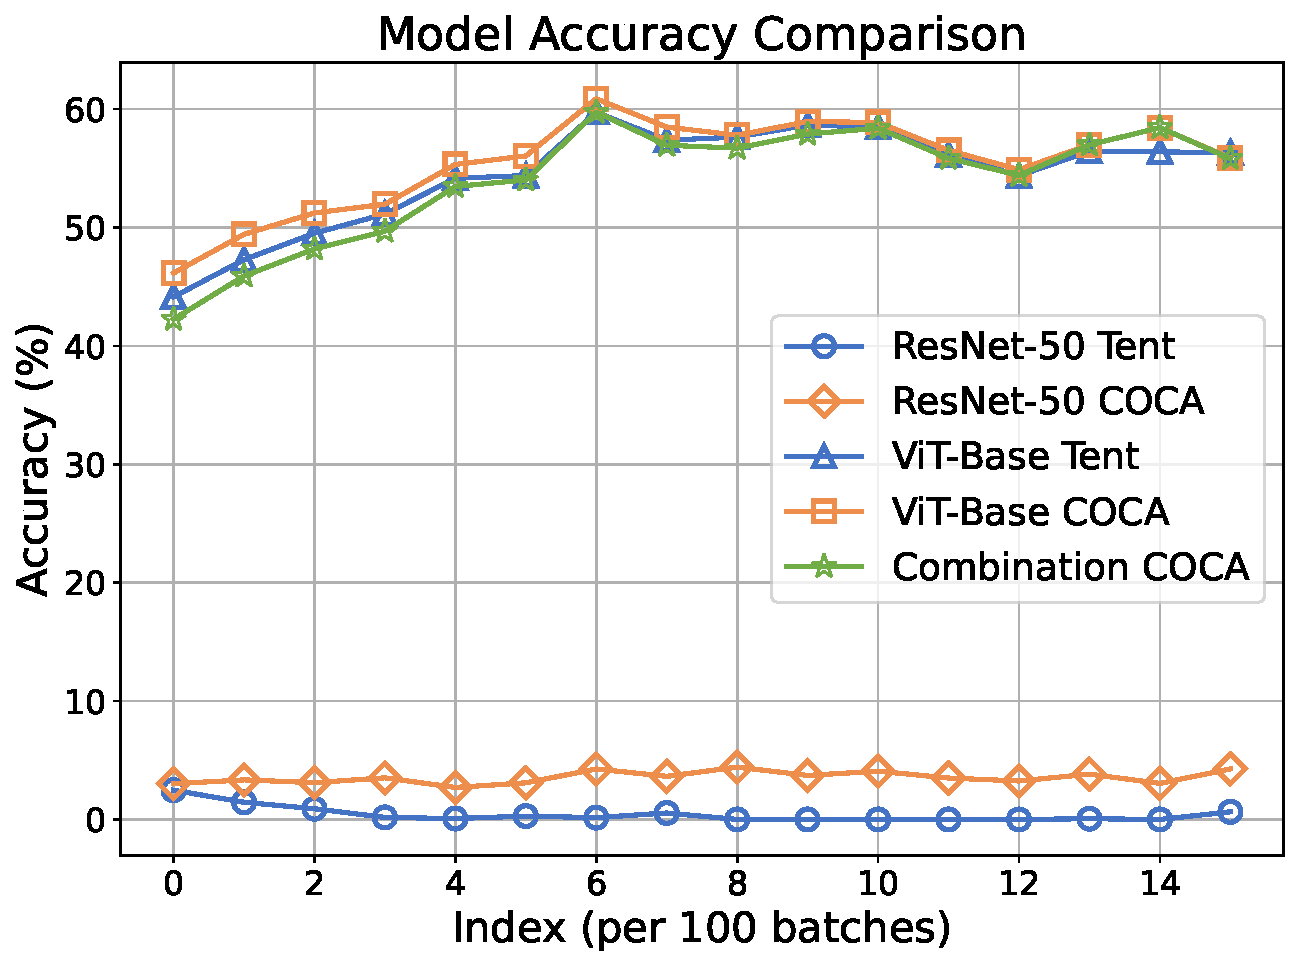
\includegraphics[width=0.85\linewidth]{sec/accuracy_comparison_updated_final.pdf}
    \vspace{-0.12in}
    \caption{Robustness of COCA stems from $\tau$. In the label-shift scenario~\cite{niu2023towards}, COCA maintains high performance even when one of the models—such as ResNet-50 in this figure—collapses. The evaluation is conducted on ImageNet-C with Gaussian noise (\%).} 
    % \vspace{-0.1in}
\label{lsrobust}
\vspace{-0.07in}
\end{figure}

\begin{table}[t]
% \vspace{-0.1in} 
    \centering
    \setlength{\tabcolsep}{9pt} % 调整列间距
    \renewcommand{\arraystretch}{1} % 增加行高(从 1 改为 1.2)
    \begin{threeparttable} % 使用 threeparttable 环境
    \resizebox{0.95\linewidth}{!}{% 
        \begin{tabular}{c|c|cc}
            % \midrule % 增加顶部的横线,使表格更整洁
            Models & \multicolumn{1}{l|}{Accuracy (\%)} & Parameters (M) & GMACs \\
            \midrule
            ResNet-18 & 35.1 & 11.7 & 1.8 \\
            ResNet-50 & 42.9 & 25.6 & 4.1 \\
            ResNet-101 & 46.5 & 44.5 & 7.8 \\
            \midrule
            Mobile-ViT & 41.0 & 10.6 & 4.1 \\
            ViT-Base & 51.7 & 86.6 & 16.9 \\
            ViT-Large & 67.8 & 304.2 & 77.8 \\
            % \midrule % 增加底部的横线
        \end{tabular}%
    }
    \vspace{-0.1in}
    \caption{Comparison of Model Profiles: performance (\%), the number of parameters (in millions), and GMACs. The performance is the average adaptation performance across 15 types of corruption on ImageNet-C, evaluated using Tent ~\cite{wang2020tent}.}
    \label{params}
    \vspace{-0.15in} 
    \end{threeparttable}
\end{table}

\vspace{-5pt}
\paragraph{The Learnable Parameter $\tau$ Enhances the Robustness of COCA}
% In Section 3, we have discussed the necessity of $\tau$, as displayed in Fig.~\ref{Tcompare}. Furthermore, introducing $\tau$ also brings robustness for COCA. In some scenarios, such as label shifts~\cite{niu2023towards}, the ResNet-50-BN model is prone to collapse. Despite this phenomenon, the collaborative model, ViT-Base, can continue to learn effectively, as shown in Fig.~\ref{lsrobust}. The accuracy based on the ResNet-50-BN model is approximately 0, indicating that the predictions of ResNet are very different from ViT. In this condition, the value of $\tau$ will become very large to balance the outputs of the two models. Based on $\tau$, the contribution provided by ResNet to collaborative knowledge computation becomes very small, as illustrated in Eq.~\ref{marginalent}, effectively preventing the impact from being harmful to collaboration since the final performance is near to ViT-Base under COCA. As a result, if one model collapses during cross-model co-learning, we can discard this model and only utilize the adapted predictions of the other model to replace the final performance. 


% In Section.\ref{sec:Method Section}, we discussed the necessity of the parameter $\tau$, as shown in Fig.~\ref{Tcompare}. Additionally, introducing $\tau$ enhances the robustness of COCA. 

As shown in Fig.~\ref{Tcompare} of section.\ref{sec:Method Section}, it is necessary to introduce a learnable parameter $\tau$, which can enhance the robustness of COCA. In certain scenarios, such as label shifts~\cite{niu2023towards}, the ResNet-50-BN model may be prone to collapse. However, in these cases, the collaborative model, ViT-Base, continues to learn effectively, as illustrated in Fig.~\ref{lsrobust}. The accuracy of the ResNet-50-BN model approaches zero, indicating that its predictions diverge significantly from those of ViT. Under such conditions, the value of $\tau$ increases substantially to balance the outputs of the two models. Consequently, the contribution of ResNet-50 to the collaborative knowledge computation diminishes, as shown in Eq.~\ref{marginalent}, thereby preventing any harmful effects on collaboration. This ensures that the final performance remains close to that of ViT-Base under COCA. Therefore, if one model collapses at test time, we can discard it and rely solely on the adapted predictions of the other model to maintain performance. In our experiments, the learnable parameter $\tau$ ranges from 1 to 5. The Appendix~\ref{VisualizeCOCA} further visualizes the benefits of COCA, highlighting how $\tau$ enables robust co-adaptation.

\vspace{-10pt}

\paragraph{Influence of Anchor Model Selection}
The influence of selecting the anchor model is shown in Table~\ref{anchorexchange}, where ``Anc." and ``Aux." refer to the accuracy of the anchor model and the auxiliary model, respectively. We observe that choosing any model as the anchor improves the performance compared to single-model TTA. Additionally, selecting a larger model as the anchor leads to better performance. Notably, the performance gap between the two models increases as the difference in the number of parameters grows. For example, when selecting ViT-Base as the anchor model, the performance is higher than when the auxiliary model is Mobile-ViT, which has fewer parameters than ResNet-50.
\begin{table}[t]
    % \vspace{-0.1in}
    \begin{center}
    \setlength{\tabcolsep}{9pt} % 调整列间距
    \renewcommand{\arraystretch}{1.1} % 增加行高
    \begin{threeparttable}
        \resizebox{\linewidth}{!}{%
            \begin{tabular}{cc|ccc}
Anchor & Auxiliary & Anc. & Aux. & \textbullet~Combined. \\ 
\midrule
ResNet-18 & ResNet-50 & 37.3 & 43.4 & 43.8 \\
ResNet-50 & ResNet-18 & 44.0 & 38.9 & \textbf{45.6} \\ \midrule
ResNet-50 & ViT-Base & 48.5 & 63.0 & 62.2 \\
ViT-Base & ResNet-50 & 63.2&50.7& \textbf{64.9} \\ \midrule
Mobile-ViT & ViT-Base & 47.7 & 63.3 & 61.6 \\
ViT-Base & Mobile-ViT & 64.0& 47.5& \textbf{64.5}
\end{tabular}%
        }
    \end{threeparttable}
    \end{center}
    \vspace{-0.25in}
    \caption{Influence of anchor model selection. Each result represents the average performance across 15 types of corruption on ImageNet-C (\%). It is clear that selecting the larger model as the anchor leads to higher performance.}
    \label{anchorexchange}
    \vspace{-0.15in}
\end{table}





% \paragraph{Effectiveness of Components in COCA }
% In our COCA, we mentioned that naively averaging the outputs combination of two models as collaborative knowledge in collaboration is infeasible, as in Fig.~\ref{Tcompare}, and thus propose a diversity-aware scaling factor $\tau$ to guide effective and stable collaborative learning and boost the adaptation performance. Based  on $\tau$, we construct the separability-enhancing marginal entropy $\mathcal{L}_{mar}$ and cross-model knowledge distillation cross-entropy $\mathcal{L}_{ckd}$. In addition to the collaborative knowledge, we also introduce self-adaptation entropy $\mathcal{L}_{sa}$ to exploit the self-knowledge of each model. We ablate them in Fig.~\ref{Tcompare} and Table.~\ref{ablation}. Firstly, using collaborative knowledge to adapt without $\tau$ performs poorer than each model's self-adaptation following Tent without collaborative knowledge, which verifies the necessity of devising an adaptive scaling factor $\tau$ for integrating collaborative knowledge. Secondly, when applying only $\mathcal{L}_{mar}$ results in 47.9\% accuracy with ResNet-50, 59.9\% with ViT-Base, and 62.5\% with the combined prediction. Meanwhile, applying only $\mathcal{L}_{ckd}$ yields 47.2\% , 59.5\% , and 61.5\% . Each of these outperforms the self-adaptation of the individual models, which suggesting that our collaborative knowledge is working well to provide valuable learning signals to models. Thirdly, Combining $\mathcal{L}_{sa}$ with either $\mathcal{L}_{ckd}$ or $\mathcal{L}_{mar}$ both lead to performance improvements compare to just using $\mathcal{L}_{mar}$ and $\mathcal{L}_{ckd}$, which illustrates the benefits of leveraging self-knowledge for collaboration. Lastly, by incorporating all the three components as the overall fitness function, our COCA achieves the best performance, \textit{i.e.},64,9\% average accuracy of 15 corruptions on ImageNet-C dataset.


% \paragraph{Effects of Anchor Model Selection in COCA} We investigate the impact of choosing different anchor models for co-learning. While selecting a larger model with more parameters might seem intuitive, we also explore the effect of choosing a less optimal anchor. From the results shown in Table.~\ref{anchorexchange}, we have the following observations. 1) Our COCA shows robustness on anchor model's choice, though choosing the models with more parameters generally enhance co-learning performance, when choosing the smaller one still shows improvement compared to using both models independently. For example, the exchange of anchor model identities between ResNet-18 and ResNet-50 resulted in an accuracy impact of 1.8\%. 2) Compared to our anchor mechanism, the pair of Mobile-ViT and ViT-Base collaborate without the anchor mechanism which perform poorer than individual adaptation shown in Fig.~\ref{Tcompare} due to the huge gap between the quantities of two models. However, COCA greatly alleviates this problem by allowing two models with a very large parameter gap to still learn well collaboratively.

% As shown in Table~\ref{anchorexchange}, the results indicate that models with more parameters generally enhance co-learning performance. For example, using ResNet-50 as the anchor model and ResNet-18 as the auxiliary results in 44.0\% accuracy for the anchor, 38.9\% for the auxiliary, and 45.6\% for the combined prediction. However, even when ResNet-18, which has significantly fewer parameters than ResNet-50, is chosen as the anchor, performance still improves compared to using both models independently (see Table.~\ref{params}). Similarly, when ViT-Base and ResNet-50 collaborate, whichever model serves as the anchor leads to better performance than when learning individually (\textit{i.e.} ViT-Base: 57.4\% $\to$ 63.0\% or 63.2\%). These results suggest that while a more powerful anchor model typically yields better performance, collaborative learning remains effective even when the anchor model is suboptimal.



\vspace{-10pt}

% \paragraph{Effectiveness of $\tau$ on robustness in Eq.~\ref{tintro} }
% In collaborative model settings, a key concern is the potential collapse of one model, which could severely disrupt collaboration and degrade overall performance. In the context of Test Time Adaptation (TTA), model collapse is indeed a risk. However, our adaptive scaling temperature mechanism ($\tau$)  effectively mitigates the impact of an auxiliary model's collapse within the COCA framework, helping to preserve the performance of the anchor model. In specific scenarios, such as label shifts introduced by SAR~\cite{niu2023towards}, the ResNet-50-BN model is prone to collapse. Despite this, the collaborative model, ViT-Base, can still continue to learn effectively, as shown in Fig.~\ref{lsrobust}. In this condition, the accuracy of ResNet-50-BN approaches to 0, which indicates the predictions of the ResNet alomst is the opposite of ViT's. At this point, as $\tau$ is learned based on diversity-aware, $\tau$ will rise to a very large value.Then, the contribution provided by ResNet to collaborative knowledge computation will become very small in Eq.~\ref{marginalent}, effectively prevent the impact of collapse model from being harmful to collaboration.

% \vspace{-10pt}


% \begin{table}[t]
%     % \vspace{-0.1in}
%     \begin{center}
%     \setlength{\tabcolsep}{9pt} % 调整列间距
%     \renewcommand{\arraystretch}{1.1} % 增加行高
%     \begin{threeparttable}
%         \resizebox{0.93\linewidth}{!}{
%             \begin{tabular}{cc|ccc}
% Anchor & Auxiliary & Anc. & Aux & \textbullet~Combined \\ \midrule
% ResNet-18\textsuperscript{1} & ResNet-18 & 31.2 & 37.4 & 38.6 \\
% ResNet-18 & ResNet-18\textsuperscript{1} & 37.2 & 31.0 & \textbf{39.9} \\ \midrule
% ResNet-50\textsuperscript{1} & ResNet-50 & 41.7 & 45.8 & 48.5 \\
% ResNet-50 & ResNet-50\textsuperscript{1} & 45.7 & 41.1 & \textbf{49.2}
% \end{tabular}%
%         }
%     \end{threeparttable}
%     \end{center}
%     \vspace{-0.23in}
%     \caption{Investigating whether COCA continues to deliver performance improvements when two models share the same deep architecture but differ in their pre-trained weights. Each result represents the average performance across 15 types of corruption on ImageNet-C (\%). For each pair, the two models have different pre-trained weights. }
%     \label{samemodel}
%     \vspace{-0.1in}
% \end{table}





% \begin{table*}[t]
    
%     \setlength{\tabcolsep}{3pt} % 调整列间距
%     \renewcommand{\arraystretch}{1.0} % 增加行高
    
%     \begin{center}
%     \begin{threeparttable}
%         \resizebox{1.0\linewidth}{!}{%
%             \begin{tabular}{c|ccc|cccc|cccc|cccc|c}
%                 \multicolumn{1}{c}{} & \multicolumn{3}{c}{Noise} & \multicolumn{4}{c}{Blur} & \multicolumn{4}{c}{Weather} & \multicolumn{4}{c}{Digital} &  \\
%                 \midrule
%                 Models & Gauss & Shot & Impul & Defoc & Glass & Motion & Zoom & Snow & Frost & Fog & Brit & Contr & Elastic & Pixel & JPEG & Avg. \\ 
%                 \midrule
%                 Mobile-ViT & 29.7 & 29.0 & 33.2 & 30.1 & 26.5 & 44.8 & 50.9 & 51.3 & 48.0 & 60.8 & 70.0 & 41.9 & 54.0 & 54.6 & 52.1 & 45.1 \\
%                 ResNet-50* & 34.0 & 35.9 & 35.7 & 32.3 & 31.5 & 45.9 & 51.1 & 50.4 & 43.8 & 59.1 & 67.9 & 41.0 & 56.5 & 59.8 & 54.4 & 46.6 \\
%                 \textbullet~Combined & \textbf{37.2} & \textbf{38.1} & \textbf{39.8} & \textbf{35.9} & \textbf{33.7} & \textbf{50.2} & \textbf{55.3} & \textbf{55.6} & \textbf{50.1} & \textbf{63.8} & \textbf{72.3} & \textbf{45.9} & \textbf{59.6} & \textbf{62.1} & \textbf{58.0} & \textbf{50.5} \\
%                 \midrule
%                 ResNet-50 & 34.6 & 37.6 & 36.7 & 32.9 & 32.7 & 47.9 & 52.5 & 51.4 & 41.1 & 59.8 & 67.4 & 22.6 & 57.9 & 60.8 & 55.7 & 46.1 \\
%                 ResNet-101* & 36.0 & 39.2 & 38.2 & 34.8 & 35.4 & 49.3 & 55.1 & 53.2 & 43.1 & 61.3 & 69.6 & 24.5 & 60.3 & 62.5 & 57.7 & 48.0 \\
%                 \textbullet~Combined & \textbf{38.7} & \textbf{41.9} & \textbf{41.0} & \textbf{36.8} & \textbf{37.0} & \textbf{52.4} & \textbf{57.3} & \textbf{55.8} & \textbf{45.1} & \textbf{63.7} & \textbf{71.3} & \textbf{25.6} & \textbf{62.5} & \textbf{65.0} & \textbf{60.1} & \textbf{50.3} \\
%                 \midrule
%                 Mobile-ViT & 32.6 & 34.7 & 35.8 & 33.1 & 32.2 & 46.9 & 50.4 & 54.0 & 51.4 & 61.4 & 70.7 & 46.5 & 55.0 & 55.0 & 53.4 & 47.5 \\
%                 ViT-Base* & \textbf{55.6} & 55.9 & 56.9 & 57.2 & \textbf{55.7} & 62.6 & 58.8 & 65.5 & 64.5 & 73.0 & 78.2 & \textbf{69.8} & 65.6 & 71.2 & 68.7 & 64.0 \\
%                 \textbullet~Combined & 55.2 & \textbf{56.0} & \textbf{57.1} & \textbf{57.3} & 55.6 & \textbf{63.5} & \textbf{61.1} & \textbf{67.3} & \textbf{65.5} & \textbf{73.7} & \textbf{78.8} & 69.0 & \textbf{67.5} & \textbf{71.3} & \textbf{68.8} & \textbf{64.5} \\
%                 \midrule
%                 Mobile-ViT & 31.6 & 34.8 & 35.3 & 32.1 & 32.0 & 47.2 & 51.9 & 53.4 & 50.8 & 61.6 & 70.3 & 45.7 & 55.1 & 55.6 & 53.1 & 47.4 \\
%                 ViT-Large* & 66.0 & 67.4 & 68.2 & 63.6 & 63.4 & 70.4 & 67.9 & 75.8 & 71.6 & 77.4 & \textbf{83.7} & 75.7 & 71.4 & 77.3 & \textbf{75.6} & 71.7 \\
%                 \textbullet~Combined & \textbf{66.4} & \textbf{67.8} & \textbf{68.6} & \textbf{64.0} & \textbf{63.8} & \textbf{70.4} & \textbf{69.0} & \textbf{76.2} & \textbf{72.4} & \textbf{77.8} & 83.4 & \textbf{76.1} & \textbf{72.8} & \textbf{76.8} & 75.2 & \textbf{72.0} \\
%                 \midrule
%                 ResNet-50 & 42.5 & 44.5 & 43.5 & 41.0 & 40.5 & 52.2 & 54.4 & 55.0 & 49.7 & 61.6 & 68.5 & 51.8 & 59.8 & 62.7 & 57.6 & 52.3 \\
%                 ViT-Large* & 66.3 & 67.7 & 68.7 & 63.8 & 64.1 & 70.9 & 68.5 & 76.0 & 71.7 & 77.5 & 83.8 & 76.1 & 71.6 & 77.8 & 75.9 & 72.0 \\
%                 \textbullet~Combined & \textbf{67.1} & \textbf{68.5} & \textbf{69.3} & \textbf{64.8} & \textbf{64.9} & \textbf{71.9} & \textbf{70.2} & \textbf{76.7} & \textbf{72.3} & \textbf{78.2} & \textbf{83.9} & \textbf{76.4} & \textbf{73.6} & \textbf{78.6} & \textbf{76.7} & \textbf{72.9} \\
%                 \midrule
%                 ViT-Base & 58.2 & 58.7 & 59.2 & 59.9 & 58.9 & 64.4 & 60.5 & 66.4 & 64.5 & 73.7 & 78.6 & 71.5 & 66.4 & 72.6 & 70.1 & 65.6 \\
%                 ViT-Large* & 66.4 & 67.5 & 68.4 & 63.8 & 63.8 & 70.5 & 66.6 & 74.3 & 71.6 & 77.1 & 83.7 & 76.1 & 70.3 & 77.4 & 75.6 & 71.5 \\
%                 \textbullet~Combined & \textbf{67.7} & \textbf{68.8} & \textbf{69.4} & \textbf{65.9} & \textbf{65.5} & \textbf{71.7} & \textbf{67.8} & \textbf{74.8} & \textbf{72.4} & \textbf{78.5} & \textbf{83.8} & \textbf{77.3} & \textbf{72.3} & \textbf{78.3} & \textbf{76.1} & \textbf{72.7} \\
%                 \midrule
%             \end{tabular}%
%         }
%     \end{threeparttable}
%     \end{center}
%     \vspace{-0.2in}
%     \caption{The performance of COCA across different model pairs, with results on ImageNet-C (\%). Additional results can be found in Appendix~\ref{allmodelsappendix}.}
%     \label{allmodels}
%     \vspace{-0.1in}
% \end{table*}





\paragraph{Performance Across Different Model Pairs \& Influence of Models' Parameters and Architectures} We first examine the performance of six models under a single-model adaptation framework following Tent~\cite{wang2020tent}, with the results shown in Table~\ref{params}. Next, we form various pairs from these models to further evaluate the applicability of COCA. As presented in Table~\ref{allmodelssup} (cf. Appendix), COCA consistently achieves robust performance across all model pairs, demonstrating that the cross-model co-learning mechanism remains effective even when the paired models share the same architecture, as in the case of ViT-Base and Mobile-ViT. Additionally, under COCA, each model consistently outperforms single-model adaptation following Tent~\cite{wang2020tent}.

From these comparative results, we derive two key insights: (1) models with a larger number of parameters tend to exhibit enhanced performance, and (2) architectural diversity offers additional benefits. Further analysis is provided in Appendix~\ref{MoreAcross}.


% Moreover, COCA remains effective even when the two models share the same deep architecture and differ only in their pre-trained weights. Table~\ref{samemodel} presents results based on ResNet-18 and ResNet-50, demonstrating that the cross-model co-learning mechanism remains robust. In this table, the superscript \textsuperscript{1} indicates that the model was pre-trained on the Instagram-1B hashtag dataset using semi-weakly supervised learning and fine-tuned on ImageNet~\cite{he2016deep}. Models without this superscript were initialized using the pre-trained weights provided by PyTorch. Notably, unlike previous findings, the performance of the anchor model does not consistently outperform that of the auxiliary model.

% \paragraph{Generalization of COCA} COCA focuses on enabling two models to collaborate and learn from each other effectively. To evaluate the generalization performance of the COCA framework, we conducted two experiments: (1) We paired six different models (three CNN-based and three Transformer-based) for collaborative learning to evaluate the improvements across various model combinations. The model profiles and co-learning results are shown in Tables~\ref{params} and \ref{allmodels}. The results demonstrate that COCA consistently improves performance across all model pairs, regardless of whether the models differ in parameter size or share similar architectures. (2) Additionally, we tested COCA with two models that share the same structure but differ in their pre-training strategies on the source domain. The results, presented in Table~\ref{samemodel}, further validate COCA's ability to enable effective co-learning across diverse models. These findings highlight that COCA is a robust and flexible strategy, well-suited for collaborative learning across a wide range of model architectures and training strategies.

\vspace{-10pt}

% \paragraph{Influence of Models' Parameters and Architectures} To further explore the factors influencing COCA's performance, we analyze the impact of model parameters and architectures. The results, summarized in Table~\ref{mainres}, Table~\ref{allmodels}, and Table~\ref{allmodelssup}, lead to the following insights: 1) More parameters enhance performance; 2) Architectural diversity offers benefits. More analysis is presented in appendix. 




% \paragraph{Influence of Models' Parameters and Architectures} To further explore the factors influencing COCA's performance, we analyze the impact of model parameters and architectures. The results, summarized in Table~\ref{mainres}, Table~\ref{allmodels}, and Table~\ref{allmodelssup}, lead to the following insights: 1) More parameters enhance performance. Increasing the parameter count in the auxiliary model enhances overall performance when the anchor model is fixed. For instance, the accuracy improves from 64.9\% with ResNet-50 and ViT-Base to 67.1\% with ResNet-101 and ViT-Base. This improvement is likely because models with more parameters and the same deep architecture can facilitate more comprehensive learning. 2) Architectural diversity offers benefits. Diversity in deep architectures between models improves performance. For pairs of models sharing one common model, the pair with differing architectures outperforms the one with similar parameter sizes but identical architectures. For example, the accuracy of ResNet-18 and ResNet-50 is 45.6\%, while Mobile-ViT and ResNet-50 achieve 50.5\%. This advantage may arise because distinct architectures enable the models to learn more diverse representations from the same source domain. 




% \begin{figure*}[t]
% \centering
%     \includegraphics[width=0.93\linewidth]{sec/samplelevel.pdf}
%     \vspace{-0.1in}
%     \caption{A sample-level analysis highlights the advantages of our proposed cross-model co-learning approach. For each sample, we select the top five predicted probabilities from both ResNet-50 and ViT-Base. However, the final correct prediction, determined by COCA, differs from each of the initial predictions.}
%     % A learnable parameter, $\tau$, is introduced to more effectively ensemble the outputs of the two models. The final predictions, $p_{com}(x)$, are derived from the combined outputs of both models.
%     \vspace{-0.1in}
% \label{samplelevel}
% \end{figure*}

% \vspace{-10pt}
\paragraph{Computational Complexity Analysis} The comparative results in Table~\ref{eff} show that COCA requires similar computational time to Tent~\cite{wang2020tent} and EATA~\cite{niu2022efficient}, while being more efficient than SAR~\cite{niu2023towards} and CoTTA~\cite{wang2022continual}. Notably, unlike CoTTA, which relies on a teacher-student framework, COCA demands less memory and GPU time. This makes COCA particularly useful when GPU resources are limited. In such cases, a smaller model like ResNet-18 can be used in place of a larger model such as ResNet-50. Although the performance may slightly decrease compared to the larger model, it can still yield satisfactory results.



% \paragraph{Ratio Between Co-adaptation and Self-adaptation} The core idea of COCA is bidirectional improvement throughout the entire adaptation process. Additionally, it is designed to be a plug-and-play module, enhancing existing TTA approaches. To keep it as simple as possible, we aim for minimal hyper-parameters. As a result, we set the ratio between co-adaptation and self-adaptation to 1:1. However, as shown in the results for \textit{EATA+COCA(ours)} in Table~\ref{cifar100c}, COCA achieves optimal performance when the ratio is set to 1:2, increasing the accuracy from 69.1\% to 69.5\%, a slight improvement. We believe that setting the ratio in Eq.~\ref{fullloss} to 1:1 represents a trade-off between slightly lower performance, but faster computation, and slightly higher performance, which requires a hyper-parameter that incurs higher computational costs.

% \begin{table}[t]
% \setlength{\tabcolsep}{11pt} % 调整列间距
%     \renewcommand{\arraystretch}{0.9} % 增加行高
% \resizebox{0.95\linewidth}{!}{%
% \begin{tabular}{c|ccc|c}

% \multicolumn{5}{c}{Sample \#1}\\ \midrule \midrule
% Model \textbackslash Class & 98 & 146 & 356 & Predicted class \\ \midrule
% ResNet-50 & 5.4 & 2.1 & 7.5 & 356 (\ding{55}) \\
% ViT-Base & 5.9 & 8.6 & 1.6 & 146 (\ding{55}) \\
% ResNet-50 / $\tau$ & 8.1 & 5.2 & 9.0 & - \\ \midrule
% Combined & 7.0 & 6.9 & 5.3 & 98 (\checkmark)\\ \midrule 
% \multicolumn{5}{c}{Sample \#2} \\ \midrule \midrule
% Model\textbackslash Class & 192 & 334 & 361 & Predicted class \\ \midrule
% ResNet-50 & 8.0 & 6.5 & 4.8 & 192 (\ding{55}) \\
% ViT-Base & 1.6 & 6.9 & 8.0 & 361 (\ding{55}) \\
% ResNet-50 / $\tau$ & 9.8 & 9.7 & 8.2 & - \\ \midrule
% Combined & 5.7 & 8.3 & 8.1 & 334 (\checkmark)
% \end{tabular}%
% }
% \vspace{-0.1in}
% \caption{Further explanation of Fig.~\ref{samplelevel} on how COCA makes accurate predictions for these two samples. The values, all less than 10, represent the predicted logits. }
% \label{Sampleleveltable}
% \vspace{-0.2in}
% \end{table}
% eata 5202 sar 5532 tent 5202 coca1 6574 coca2 10,531 cotta 17,211

\begin{table}[t]
    % \vspace{-0.05in}
    \begin{center}
    \setlength{\tabcolsep}{3pt} % 调整列间距
    \renewcommand{\arraystretch}{1} % 增加行高
    \begin{threeparttable}
        \resizebox{\linewidth}{!}{%
            \begin{tabular}{l|c|cc}
\multicolumn{1}{c|}{Methods} & Accuracy (\%) & GPU Time (s) & Memory Usage \\ \midrule
Source Only & 35.0 & 115 & 1300 \\ \midrule
CoTTA~\cite{wang2022continual} & 56.7 & 724 & 17,211 \\
Tent~\cite{wang2020tent} & 51.7 & 234 & 5202 \\
SAR~\cite{niu2023towards} & 51.9 & 472 & 5532 \\
EATA~\cite{niu2022efficient} & 55.6 & 246 & 5202 \\
DeYO~\cite{lee2024entropy} & 54.1 & 318 & 5371 \\ 
ROID~\cite{marsden2024universal2} & 52.0 & 371 & 7972 \\ \midrule
\textbf{COCA\textsuperscript{1} (ours)}& 56.8 & 315 & 6574 \\
\textbf{COCA\textsuperscript{1} (ours)} +~EATA & \textbf{59.7} & 316 & 6574 \\ \midrule
\textbf{COCA\textsuperscript{2} (ours)}& 58.3 & 317 & 10,531 \\
\textbf{COCA\textsuperscript{2} (ours)} +~EATA & \textbf{60.9} & 319 & 10,531



\end{tabular}%
        }
    \end{threeparttable}
    \end{center}
    \vspace{-0.23in}
    \caption{Computational complexity analysis. COCA¹ and COCA² denote the collaborations between ResNet-18 and ViT-Base, and between ResNet-50 and ViT-Base, respectively. The results are based on ImageNet-C (Gaussian noise).}
    \label{eff}
    \vspace{-0.15in}
\end{table}
% The results are based on ImageNet-C (Gaussian noise). 

\vspace{-7pt}


\paragraph{Rethinking the Advantages of COCA} The consistent superiority of COCA can be attributed to the fact that, when dealing with out-of-distribution data, the two models leverage their unique strengths to collaboratively achieve robust performance. COCA serves as a general framework for cross-model co-learning, allowing a smaller model like MobileViT to effectively guide a larger model like ViT-Base. Furthermore, the co-adaptation between edge models like ResNet-18 and MobileViT surpasses the performance of much larger models such as ResNet-101 (Table~\ref{params}, Table~\ref{allmodelssup} in Appendix), offering valuable insights for tackling resource-constrained tasks. Additionally, COCA updates the parameters of both models simultaneously without causing a significant increase in GPU time (Table~\ref{eff}). 
% —often outperforming that of a larger model
% Additionally, COCA offers a flexible performance-efficiency trade-off by incorporating a smaller auxiliary model like ResNet-18.
\vspace{-7pt}
\paragraph{Is COCA Applicable to More Than Two Models?}
Building on COCA’s mechanism, a new question emerges: Is COCA applicable to multiple models? In particular, can incorporating a third small model further improve the TTA performance? To answer this, we verify our effectiveness across multiple models in Appendix~\ref{suppl:sec:three-models}, which showcases COCA's consistent improvement in overall accuracy with more collaborating models, underscoring our scalability. Results and analyses are detailed in Appendix~\ref{suppl:sec:three-models}.

% Building on COCA’s outstanding performance, a new question emerges: Is COCA applicable to multiple models? In particular, does incorporating a third small model to collaborate with an existing pair of small models further enhance overall performance? We verify our effectiveness across multiple models in Appendix~\ref{suppl:sec:three-models}, which showcases that COCA consistently improves the overall accuracy with more collaborating models. Detailed results and analyses are provided in Appendix~\ref{suppl:sec:three-models}.


% Detailed results and analyses in Appendix provide affirmative answers to both questions.

% The general procedure follows a similar structure to the pseudocode outlined in Algorithm 1 in appendix. Given three models, denoted as M1, M2, and M3, we rank them by size in descending order: M1 $>$ M2 $>$ M3. The co-learning process is conducted in two steps: 1) M2 and M3 are designated as the anchor model and auxiliary model, respectively. COCA is trained using these two models. 2) M1 and the combination of M2 and M3 are designated as the anchor model and auxiliary model, respectively. The detailed results and analysis, proving COCA's applicability to more than two models, are presented in appendix.

% \paragraph{Visualizing the Advantages of COCA} Extensive comparative results demonstrate that COCA consistently outperforms a single model. To further illustrate this advantage, we present two sample cases where, even if individual models make incorrect predictions, their combined output can still yield the correct result. Specifically, we examine Sample 1 and Sample 2 to showcase COCA's benefits. As shown in Fig.\ref{samplelevel}, both the ViT-Base and ResNet-50 models confidently produce incorrect predictions, with the assigned probability for the predicted category significantly higher than for the others. In contrast, our proposed approach, COCA, generates entirely different but correct predictions. Additionally, we use these two samples to explain why COCA can make accurate predictions, leveraging the learnable parameter $\tau$, as detailed in Table\ref{Sampleleveltable}. The combined logit is the average of the logits from ViT-base and the logits from ResNet-50, where the latter is scaled by a factor of $\tau$. Take the predicted logits for category 192 as an example: $5.7 = (1.6 + 9.8) / 2$.
% \vspace{-10pt}


% \begin{table}[h]
% \setlength{\tabcolsep}{11pt} % 调整列间距
%     \renewcommand{\arraystretch}{0.9} % 增加行高
% \resizebox{0.95\linewidth}{!}{%
% \begin{tabular}{c|ccc|c}
% Model\textbackslash Class & 192 & 334 & 361 & Predicted \\ \midrule
% ResNet-50 & 8.0 & 6.5 & 4.8 & 192 (\ding{55}) \\
% ViT-Base & 1.6 & 6.9 & 8.0 & 361 (\ding{55}) \\
% ResNet-50 / $\tau$ & 9.8 & 9.7 & 8.2 & 192 (\ding{55}) \\ \midrule
% Combined & 5.7 & 8.3 & 8.1 & 334 (\checkmark)
% \end{tabular}%
% }
% \caption{Further illustration of sample-level predictions based on the sample's original predicted logits.}
% \label{Sample1}
% \end{table}
% (1) In the collaboration of models, keeping the anchor model unchanged improves performance as the quantity of auxiliary model parameter increases(\textit{i.e.} ResNet-50 + ViT-Base gain 64.9\% combination accuracy $\rightarrow$ ResNet-101 + ViT-Base gain 67.1\% combination accuracy). (2) When models have similar number of parameters, COCA achieves better performance enhancement when the models have different architectures(\textit{i.e.} ResNet-18 + ResNet-50 gain 45.6\% combination accuracy $\rightarrow$ Mobile-ViT+ ResNet-50 gain 50.5\% combination accuracy). In summary, collaborative learning between models with different architectures generally leads to stronger performance, even when their parameter counts are similar, due to the models with different structures learned widely varying knowledge in the source domains. On the other hand, for models with the same architecture, a larger number of parameters typically reflects more comprehensive learning in the source domain, but there is still potential for improvement through collaboration.


% \paragraph{Comparison on Additional Datasets} We also evaluated COCA on two more challenging datasets, ImageNet-R and ImageNet-Sketch\cite{hendrycks2021many}, which involve natural distribution shifts. As shown in Table~\ref{RSdatasets}, COCA consistently delivers significant performance improvements, both when using simple entropy minimization and when combined with other TTA methods. This success can be attributed to COCA's ability to effectively facilitate model collaboration.
 % Acc. (\%, $\uparrow$)
% \paragraph{Comparison with Teacher-Student TTA methods }When it comes to the collaboration of two models in our proposed COCA, the most related framework to us is based on teacher-student network. In recent TTA methods, CoTTA \cite{wang2022continual} use teacher-student networks as the framework for the method. Therefore, we compared COCA with CoTTA, and results are shown in Table. \ref{eff}. From the results, we can see that COCA exhibits significant performance advantages and greatly reduces the cost of memory.
% \vspace{-11pt}\paragraph{Computational Complexity Analysis} In the COCA framework, two models collaborate for adaptation, a concept similar to the teacher-student networks used in recent TTA methods like CoTTA \cite{wang2022continual}.Thus, we compared COCA with CoTTA and other TTA methods, as shown in Table~\ref{eff}. The results demonstrate that COCA not only outperforms CoTTA in terms of adaptation accuracy (58.3\% $vs.$ 56.7\%), but also significantly reduces memory usage, requiring only 11,422 MiB compared to CoTTA's 19,979 MiB. Additionally, COCA achieves this performance with a reasonable computational GPU time of 317 seconds, highlighting its suitability for real-world applications. Moreover, COCA allows for flexibility in model selection, which enabling users to pair different auxiliary models to reduce memory usage without substantial performance degradation (e.g., ResNet-50 + ViT-Base → ResNet-18 + ViT-Base).
% \vspace{-0.35in}


% \textbf{Is COCA applicable on multi-models?} The experimental results indicate that two models can learn from each other and produce better performance. Thus, can more models further increase the performance?

\vspace{6pt}
\section{Conclusions}
% \vspace{-2pt}
In this paper, we aim to investigate the co-learning mechanism to enhance test-time adaptation (TTA). Notably, we uncover two key insights regarding different models: 1) They provide complementary knowledge from training, and 2) They exhibit varying robustness against noisy learning signals during testing. To this end, we propose COCA, a co-learning TTA approach that promotes bidirectional cooperation across models. COCA integrates complementary knowledge to mitigate biases and enables tailored adaptation strategies for each model’s strengths. Notably, a learnable temperature, $\tau$, is introduced to align the outputs from models of different sizes. Extensive experiments validate COCA's effectiveness across diverse models and offer new insights into TTA. For example, we show that a smaller model like ResNet-18, attributed to its robustness to noise at testing, can significantly enhance the TTA of a much larger model like ViT-large. 
% Moreover, collaboration between models with different architectures yields the most substantial performance gains. 
Additionally, COCA can also serve as a plug-and-play module that seamlessly complements traditional TTA methods for more effective and robust solutions. 

% Finally, we also verify COCA's applicability to multiple models, which leads to a consistent improvement in overall accuracy .

% 
% aligns the outputs of models with varying sizes and explores the complementary knowledge of a smaller model to enhance a larger model, ensuring a more effective and robust adaptation process.

% Extensive experiments validate COCA's effectiveness across diverse models and offer new insights into test-time adaptation (TTA). For example, a smaller model like ResNet-18, known for its robustness to noisy guidance at test time, can significantly guide a larger model such as ViT-large. Moreover, collaboration between models with different architectures yields the most substantial performance gains. Additionally, COCA can also serve as a plug-and-play module that can seamlessly complement traditional TTA methods, further enhancing their effectiveness. COCA's applicability to multiple models is also confirmed.




% In this paper, we introduce COCA, a novel test-time adaptation (TTA) approach that leverages cross-model collaboration to significantly enhance model performance. Unlike traditional one-way methods, such as the teacher-student framework, COCA fosters bi-directional cooperation between models, enabling mutual performance improvements. COCA not only integrates complementary knowledge from different models to mitigate individual biases, but also enables diverse adaptation strategies tailored to each model's unique strengths. Moreover, To enhance knowledge aggregation and co-adaptation, we introduce a learnable parameter $\tau$, which aligns the outputs of models with different sizes, ensuring a more effective and robust adaptation process. 

% Our experiments demonstrate that collaboration between models with different architectures yields the greatest performance gains. Smaller models not only boost the performance of larger models but also achieve notable improvements in their own accuracy. These findings highlight the potential of model collaboration and output integration in driving substantial performance improvements. COCA is a versatile framework that can seamlessly complement traditional TTA methods, boosting their effectiveness. Furthermore, the applicability of COCA across multiple models is also confirmed, as detailed in Section D of appendix. Through extensive experiments and analysis, we provide valuable insights into TTA and cross-model co-learning, offering a fresh perspective on overcoming the limitations of conventional adaptation techniques.


% In this paper, we introduce COCA, a novel test-time adaptation (TTA) approach that leverages cross-model collaboration to significantly enhance model performance. Unlike traditional one-way methods, such as the teacher-student framework, COCA promotes bi-directional cooperation between models, enabling mutual performance improvements. Our experiments demonstrate that collaboration between models with different architectures yields the greatest performance gains. Smaller models not only enhance the performance of larger models but also show notable improvements in their own accuracy. Additionally, we introduce a unique adaptive temperature scaling parameter to combine model outputs, resulting in further performance enhancements. These findings highlight the potential of model collaboration and output integration to achieve substantial performance gains. COCA is also a versatile framework that can seamlessly integrate with traditional TTA methods, boosting their effectiveness. Through extensive experiments and analysis, we offer valuable insights into TTA and cross-model co-learning, presenting a fresh perspective on overcoming the limitations of conventional adaptation techniques.

% \newpage
{
    \small
    \bibliographystyle{ieeenat_fullname}
    \bibliography{main}
}

\clearpage
\setcounter{page}{1}
\maketitlesupplementary
% Comparison of accuracy (%) on ImageNet-C (level 5) with pairwise collaboration of all models
% In the supplementary materials, we provide additional experimental results and further details of our proposed approach, COCA. 
% We also explore the applicability of COCA across multiple models. 
\appendix
\section{Pseudo-code of COCA}
\label{pscode}
\begin{algorithm}
\begin{spacing}{1.1}
\caption{The pipeline of proposed COCA.}
\label{alg:coca}
\textbf{Input:} Test samples $D^{\text{test}}=\{x_j\}_{j=1}^M$, the pre-trained models $f_{\theta_{1}}, f_{\theta_{2}}$ with trainable parameters $\widetilde{\theta}_{1}, \widetilde{\theta}_{2} \subseteq  \theta_{1}, \theta_{2}$, steps $K$ for learnable $\tau$.
\begin{algorithmic}[1]

    \STATE Initialize $\tau = 1 $
    \FOR{each batch of test samples }
        \STATE Calculate predictions $\hat{y}_{\theta_{1}}$ $\hat{y}_{\theta_{2}}$ via ${f}
        _{\theta_{1}}$ and ${f}_{\theta_{2}}$
        \FOR{ $i=1 $ \textbf{to} $ K$}
        % \WHILE{$i \le K$} 
            \STATE Update $\tau$ via Eqn.(\ref{tloss})
        \ENDFOR
        \STATE Calculate combined predictions $\hat{y}_{e}$ via Eqn.(\ref{tau_ensemble})
        \STATE Calculate co-adaptation loss $\mathcal{L}_{col}$ via Eqn.(\ref{colloss})
        \STATE Calculate self-adaptation loss $\mathcal{L}_{sa}$ via Eqn.(\ref{selfloss})
        \STATE Update $\widetilde{\theta}_{1}$ and $\widetilde{\theta}_{2}$ via Eqn.(\ref{fullloss})
        
    \ENDFOR 
\end{algorithmic}
\textbf{Output:} Predictions $\{ \hat{y}^j_{\theta_{1}}, \hat{y}^j_{\theta_{2}},\hat{y}^j_e\}_{j=1}^M $ for all $x_{j} \in D^{\text{test}}$.
% \textbf{Output:} The predictions $\{ \hat{y}^j_{\theta_{1}}, \hat{y}^j_{\theta_{2}},\hat{y}^j_e\}_{j=1}^M $ for all $x \in D_{\text{test}}$.
\end{spacing}
\end{algorithm}

% Additional Experimental Results Exploring the Applicability of COCA Across Different Pairs of Deep Architectures

\section{Implementation Details of COCA Integrated with Baseline Methods}
\label{imdeatils}
As discussed in the main manuscript, COCA can also serve as a plug-and-play module to enhance existing TTA methods by applying its loss function (Eq.~\ref{fullloss}). For instance, \textit{EATA~\cite{niu2022efficient} + COCA} utilizes EATA's sample filtering and weighting mechanism to compute both the self-adaptation loss for individual models and the co-adaptation loss for selected model pairs. Similarly, \textit{SAR~\cite{niu2023towards} + COCA} employs the Sharpness-Aware Minimization (SAM) optimizer from SAR's original formulation to jointly optimize model parameters while integrating its entropy-based reliability filtering mechanism. Moreover, the implementation details of all the baseline methods follow their original implementation formulations.

\section{The Study of Step $K$ for Updating the Learnable Parameter $\tau$}
\label{kstudy}
In Section~\ref{sec:Method Section} of the main paper, we introduced the temperature-scaled parameter $\tau$  to facilitate the combination of two models. We now examine how to determine the optimal value of $\tau$, which is governed by the parameter $K$ (the number of updating steps). The results, shown in Table~\ref{tepoch}, indicate that only a small number of epochs—approximately 3 to 5—are needed to achieve the optimal value of $\tau$. Furthermore, these results demonstrate that COCA is not highly sensitive to the choice of $K$. Note that we apply stop gradients to the model outputs and update only the parameter $\tau$, without performing backpropagation. As a result, learning $\tau$ incurs negligible computational cost, even with a large number of update steps $K$, ensuring efficient adaptation.





\section{Visualizing the Advantages of COCA}
\label{VisualizeCOCA}
Extensive comparative results demonstrate that COCA consistently outperforms a single model. To further illustrate this advantage, we present two sample cases where, even if individual models make incorrect predictions, their combined output can still yield the correct result. Specifically, we examine Sample \#1 and Sample \#2 to showcase COCA's benefits. As shown in Fig.\ref{samplelevel}, both the ViT-Base and ResNet-50 models confidently produce incorrect predictions, with the assigned probability for the predicted category significantly higher than for the others. In contrast, our proposed approach, COCA, generates entirely different but correct predictions. Additionally, we use these two samples to explain why COCA can make accurate predictions, leveraging the learnable parameter $\tau$, as detailed in Table~\ref{Sampleleveltable}. The combined logit is the average of the logits from ViT-base and the logits from ResNet-50, where the latter is scaled by a factor of $\tau$. Take the predicted logits for category 192 as an example: $5.7 = (1.6 + 9.8) / 2$.

\begin{table}[t]
    % \vspace{-0.1in}
     \setlength{\tabcolsep}{6pt} % 调整列间距
    \renewcommand{\arraystretch}{1.1} % 增加行高
    \begin{center}
    \begin{threeparttable}
        \resizebox{0.95\linewidth}{!}{%
            \begin{tabular}{l|cc|c}
                \multicolumn{1}{c|}{Methods} & ImageNet-R & ImageNet-Sketch & Avg.  \\
                \midrule
                Tent~\cite{wang2020tent} & 54.2 & 32.5 & 43.4 \\
                CoTTA~\cite{wang2022continual} & 56.6 & 42.4 & 49.5 \\
                \textbf{COCA (ours)} & \textbf{57.7} & \textbf{44.0} & \textbf{50.9} \\
                \midrule
                EATA~\cite{niu2022efficient} & 55.4 & 40.0 & 47.7 \\
                EATA +~\textbf{COCA (ours)} & \textbf{63.8} & \textbf{47.8} & \textbf{55.8} \\
                \midrule
                SAR~\cite{niu2023towards} & 55.0 & 33.8 & 44.4 \\
                SAR +~\textbf{COCA (ours)} & \textbf{60.7} & \textbf{44.4} & \textbf{52.6} \\
                % \midrule % 增加底部的横线
            \end{tabular}%
        }
    \end{threeparttable}
    \end{center}
    \vspace{-0.25in}
    \caption{Comparative results (\%) on the real-world datasets ImageNet-R and ImageNet-Sketch show that COCA consistently outperforms all baseline methods. Additionally, COCA functions as a plug-and-play module that significantly enhances entropy-based TTA methods, such as EATA~\cite{niu2022efficient} and SAR~\cite{niu2023towards}.}
    \vspace{-0.15in}
    \label{RSdatasets}

\end{table}

\begin{figure*}[t]
\centering
    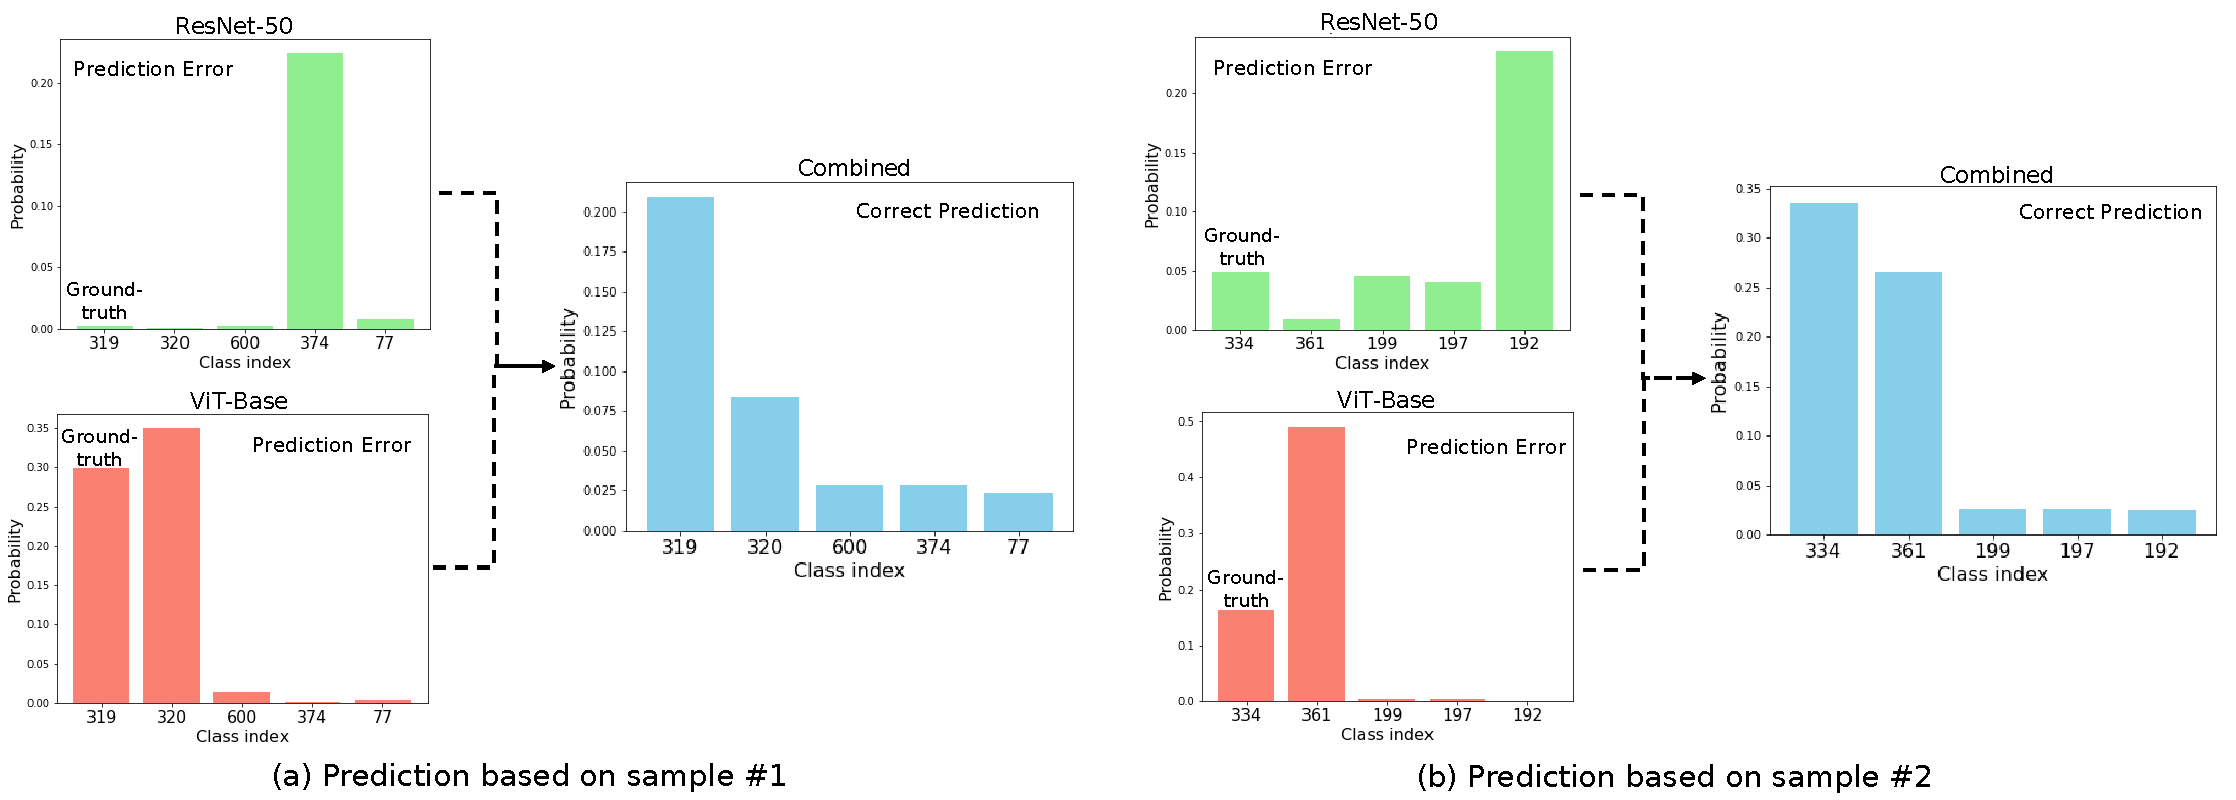
\includegraphics[width=0.93\linewidth]{sec/samplelevelvision.pdf}
    \vspace{-0.1in}
    \caption{A sample-level analysis highlights the advantages of our proposed cross-model co-learning approach. For each sample, we select the top five predicted probabilities from both ResNet-50 and ViT-Base. However, the final correct prediction, determined by COCA, differs from each of the initial predictions.}
    % A learnable parameter, $\tau$, is introduced to more effectively ensemble the outputs of the two models. The final predictions, $p_{com}(x)$, are derived from the combined outputs of both models.
    \vspace{-0.1in}
\label{samplelevel}
\end{figure*}


\section{Ratio Between Co-adaptation and Self-adaptation}
\label{Ratio}
COCA is designed to foster bidirectional improvement throughout the entire adaptation process. It can also be seamlessly integrated as a plug-and-play module to boost existing Test-Time Adaptation (TTA) methods. To keep our approach as simple as possible, we minimize the number of hyper-parameters, initially setting the co-adaptation to self-adaptation ratio to 1:1 as indicated in Eq.~\ref{fullloss}. Further experiments with \textit{EATA+COCA (ours)} on ImageNet-C reveal that a ratio of 1:2 slightly enhances accuracy—from 69.1\% to 69.5\%. Therefore, we view the 1:1 setting as a balanced compromise, offering faster computation with a modest performance trade-off compared to the marginal gains achieved with a higher computational cost.


\begin{table}[t]
\setlength{\tabcolsep}{11pt} % 调整列间距
    \renewcommand{\arraystretch}{0.9} % 增加行高
\resizebox{0.95\linewidth}{!}{%
\begin{tabular}{c|ccc|c}

\multicolumn{5}{c}{Sample \#1}\\ \midrule \midrule
Model \textbackslash Class & 98 & 146 & 356 & Predicted class \\ \midrule
ResNet-50 & 5.4 & 2.1 & 7.5 & 356 (\ding{55}) \\
ViT-Base & 5.9 & 8.6 & 1.6 & 146 (\ding{55}) \\
ResNet-50 / $\tau$ & 8.1 & 5.2 & 9.0 & - \\ \midrule
Combined & 7.0 & 6.9 & 5.3 & 98 (\checkmark)\\ \midrule 
\multicolumn{5}{c}{Sample \#2} \\ \midrule \midrule
Model\textbackslash Class & 192 & 334 & 361 & Predicted class \\ \midrule
ResNet-50 & 8.0 & 6.5 & 4.8 & 192 (\ding{55}) \\
ViT-Base & 1.6 & 6.9 & 8.0 & 361 (\ding{55}) \\
ResNet-50 / $\tau$ & 9.8 & 9.7 & 8.2 & - \\ \midrule
Combined & 5.7 & 8.3 & 8.1 & 334 (\checkmark)
\end{tabular}%
}
\vspace{-0.1in}
\caption{Further explanation of Fig.~\ref{samplelevel} on how COCA makes accurate predictions for these two samples. The values, all less than 10, represent the predicted logits. }
\label{Sampleleveltable}
\vspace{-0.2in}
\end{table}
% \


\section{The Influence of Model Weights}
\label{weights}
COCA remains effective even when the two models share the same deep architecture and differ only in their pre-trained weights. Table~\ref{samemodel} presents results based on ResNet-18 and ResNet-50, demonstrating that the cross-model co-learning mechanism remains robust. In this table, the superscript \textsuperscript{1} indicates that the model was pre-trained on the Instagram-1B hashtag dataset using semi-weakly supervised learning and fine-tuned on ImageNet~\cite{he2016deep}. Models without this superscript were initialized using the pre-trained weights provided by PyTorch. Notably, unlike previous findings, the performance of the anchor model does not consistently outperform that of the auxiliary model.



\begin{table}[t]
    % \vspace{-0.1in}
    \begin{center}
    \setlength{\tabcolsep}{9pt} % 调整列间距
    \renewcommand{\arraystretch}{1.1} % 增加行高
    \begin{threeparttable}
        \resizebox{\linewidth}{!}{
            \begin{tabular}{cc|ccc}
Anchor & Auxiliary & Anc. & Aux & \textbullet~Combined \\ \midrule
ResNet-18\textsuperscript{1} & ResNet-18 & 31.2 & 37.4 & 38.6 \\
ResNet-18 & ResNet-18\textsuperscript{1} & 37.2 & 31.0 & \textbf{39.9} \\ \midrule
ResNet-50\textsuperscript{1} & ResNet-50 & 41.7 & 45.8 & 48.5 \\
ResNet-50 & ResNet-50\textsuperscript{1} & 45.7 & 41.1 & \textbf{49.2}
\end{tabular}%
        }
    \end{threeparttable}
    \end{center}
    \vspace{-0.23in}
    \caption{Investigating whether COCA continues to deliver performance improvements when two models share the same deep architecture but differ in their pre-trained weights. Each result represents the average performance across 15 types of corruption on ImageNet-C (\%). For each pair, the two models have different pre-trained weights. }
    \label{samemodel}
    \vspace{-0.15in}
\end{table}



% section{Comparative Results on Cifar100-C dataset}
% \label{Cifar100-C}


\begin{table*}[t]
    \setlength{\tabcolsep}{3pt} % 调整列间距
    \renewcommand{\arraystretch}{1.1} % 增加行高
\resizebox{1.0\linewidth}{!}{%
\begin{tabular}{lccccccccccccccccc}
\multicolumn{1}{c}{} &  & \multicolumn{3}{c}{Noise} & \multicolumn{4}{c}{Blur} & \multicolumn{4}{c}{Weather} & \multicolumn{4}{c}{Digital} &  \\ \midrule
\multicolumn{1}{c|}{Methods} & \multicolumn{1}{c|}{Models} & Gauss & Shot & \multicolumn{1}{c|}{Impul} & Defoc & Glass & Motion & \multicolumn{1}{c|}{Zoom} & Snow & Frost & Fog & \multicolumn{1}{c|}{Brit} & Contr & Elastic & Pixel & \multicolumn{1}{c|}{JPEG} & Avg. \\ \midrule
\multicolumn{1}{l|}{\multirow{2}{*}{Source Only}} & \multicolumn{1}{c|}{ResNet-50} & 4.1 & 4.8 & \multicolumn{1}{c|}{2.0} & 26.1 & 11.2 & 26.1 & \multicolumn{1}{c|}{31.3} & 6.9 & 14.4 & 40.4 & \multicolumn{1}{c|}{9.6} & 36.9 & 20.1 & 11.5 & \multicolumn{1}{c|}{13.6} & 17.3 \\
\multicolumn{1}{l|}{} & \multicolumn{1}{c|}{ViT-Base} & 24.5 & 28.7 & \multicolumn{1}{c|}{29.4} & 59.6 & 23.3 & 53.1 & \multicolumn{1}{c|}{63.6} & 56.9 & 57.7 & 67.2 & \multicolumn{1}{c|}{70.6} & 76.2 & 45.3 & 36.2 & \multicolumn{1}{c|}{50.5} & 49.5 \\ \midrule
\multicolumn{1}{l|}{\multirow{2}{*}{Tent~\cite{wang2020tent}}} & \multicolumn{1}{c|}{ResNet-50} & 32.4 & 34.9 & \multicolumn{1}{c|}{33.2} & 64.9 & 38.7 & 61.0 & \multicolumn{1}{c|}{67.7} & 59.5 & 58.8 & 61.0 & \multicolumn{1}{c|}{73.3} & 67.0 & 51.8 & 59.7 & \multicolumn{1}{c|}{43.6} & 53.8 \\
\multicolumn{1}{l|}{} & \multicolumn{1}{c|}{ViT-Base} & 49.9 & 52.6 & \multicolumn{1}{c|}{56.1} & 76.5 & 32.5 & 71.5 & \multicolumn{1}{c|}{77.9} & 77.7 & 76.1 & 71.8 & \multicolumn{1}{c|}{88.9} & 74.3 & 58.5 & 42.8 & \multicolumn{1}{c|}{66.3} & 64.8 \\ \midrule
\multicolumn{1}{l|}{\multirow{2}{*}{EATA~\cite{niu2022efficient}}} & \multicolumn{1}{c|}{ResNet-50} & 35.5 & 37.4 & \multicolumn{1}{c|}{36.9} & 33.5 & 32.9 & 46.8 & \multicolumn{1}{c|}{52.5} & 51.6 & 45.8 & 60.0 & \multicolumn{1}{c|}{68.6} & 42.4 & 58.0 & 60.9 & \multicolumn{1}{c|}{55.5} & 55.4 \\
\multicolumn{1}{l|}{} & \multicolumn{1}{c|}{ViT-Base} & 54.1 & 54.8 & \multicolumn{1}{c|}{55.0} & 54.0 & 54.6 & 61.6 & \multicolumn{1}{c|}{57.8} & 63.5 & 62.8 & 71.3 & \multicolumn{1}{c|}{77.0} & 66.8 & 64.6 & 71.4 & \multicolumn{1}{c|}{68.1} & 66.7 \\ \midrule
\multicolumn{1}{l|}{\multirow{2}{*}{ROID~\cite{marsden2024universal2}}} & \multicolumn{1}{c|}{ResNet-50} & 36.2 & 39.5 & \multicolumn{1}{c|}{33.4} & 66.2 & 39.3 & 63.6 & \multicolumn{1}{c|}{68.0} & 62.5 & 62.2 & 64.8 & \multicolumn{1}{c|}{75.8} & 70.4 & 51.7 & 58.4 & \multicolumn{1}{c|}{42.4} & 55.6 \\
\multicolumn{1}{l|}{} & \multicolumn{1}{c|}{ViT-Base} & 55.6 & 57.9 & \multicolumn{1}{c|}{61.2} & 75.2 & 48.1 & 71.9 & \multicolumn{1}{c|}{77.1} & 73.3 & 75.5 & 76.4 & \multicolumn{1}{c|}{83.7} & 84.2 & 64.5 & 68.6 & \multicolumn{1}{c|}{64.4} & 69.2 \\ \midrule
\multicolumn{1}{l|}{\multirow{2}{*}{DeYO~\cite{lee2024entropy}}} & \multicolumn{1}{c|}{ResNet-50} & 35.9 & 39.4 & \multicolumn{1}{c|}{32.3} & 66.7 & 39.3 & 63.4 & \multicolumn{1}{c|}{68.1} & 62.4 & 61.7 & 65.1 & \multicolumn{1}{c|}{75.7} & 71.3 & 51.8 & 58.2 & \multicolumn{1}{c|}{42.2} & 55.6 \\
\multicolumn{1}{l|}{} & \multicolumn{1}{c|}{ViT-Base} & 49.6 & 52.7 & \multicolumn{1}{c|}{58.4} & 76.0 & 42.8 & 72.8 & \multicolumn{1}{c|}{76.7} & 73.9 & 74.3 & 75.9 & \multicolumn{1}{c|}{85.0} & 83.1 & 62.0 & 62.5 & \multicolumn{1}{c|}{62.6} & 67.2 \\ \midrule
\multicolumn{1}{l|}{\textbf{COCA\textsuperscript{1} (ours)}} & \multicolumn{1}{c|}{Combined} & 52.3 & 48.4 & \multicolumn{1}{c|}{65.6} & 81.2 & 55.1 & 79.5 & \multicolumn{1}{c|}{82.4} & 79.7 & 79.2 & 79.9 & \multicolumn{1}{c|}{88.2} & 87.2 & 69.1 & 77.1 & \multicolumn{1}{c|}{68.6} & 72.9 \\
\multicolumn{1}{l|}{\textbf{COCA\textsuperscript{2} (ours)}} & \multicolumn{1}{c|}{Combined} & \textbf{62.1} & \textbf{64.5} & \multicolumn{1}{c|}{\textbf{70.0}} & \textbf{82.4} & \textbf{61.8} & \textbf{80.1} & \multicolumn{1}{c|}{\textbf{82.3}} & \textbf{79.9} & \textbf{80.8} & \textbf{81.0} & \multicolumn{1}{c|}{\textbf{88.5}} & \textbf{87.5} & \textbf{71.9} & \textbf{77.6} & \multicolumn{1}{c|}{\textbf{69.4}} & \textbf{76.0}\\ \midrule
\end{tabular}
}
\vspace{-0.1in}
    \caption{Comparative results based on the Cifar100-C dataset (\%). COCA¹ and COCA² refer to the collaborations between ResNet-18 and ViT-Base, and between ResNet-50 and ViT-Base, respectively.}
    \label{cifar100c}
    % \vspace{-0.1in}

\end{table*}

\begin{table*}[t]
    \setlength{\tabcolsep}{8pt} % 调整列间距
    \renewcommand{\arraystretch}{1} % 增加行高
    
    \begin{center}
    \begin{threeparttable}
    \resizebox{1\linewidth}{!}{%
\begin{tabular}{c|ccccccccccc}
Model / Steps & $K=0$ & $K=1$ & $K=2$ & $K=3$ & $K=4$ & $K=5$ & $K=6$ & $K=7$ & $K=8$ & $K=9$ & $K=10$ \\ \midrule
ResNet-18 & 27.6 & 29.5 & 29.5 & 29.4 & 29.4 & 29.5 & 29.2 & 29.5 & 29.4 & 29.0 & 29.2 \\
ResNet-50* & 32.1 & 32.8 & 32.6 & 32.6 & 32.6 & 32.8 & 32.4 & 32.6 & 32.6 & 32.5 & 32.5 \\
\textbullet~Combined & 33.3 & 35.2 & 35.1 & 35.1 & 35.1 & 35.2 & 34.8 & 35.1 & 35.1 & 35.0 & 35.0 \\ \midrule
Mobile-ViT & 32.1 & 32.5 & 32.7 & 32.2 & 32.5 & 32.1 & 32.5 & 32.3 & 32.4 & 32.4 & 32.5 \\
ViT-Base* & 54.8 & 55.5 & 55.5 & 55.6 & 55.6 & 55.6 & 55.6 & 55.6 & 55.5 & 55.5 & 55.6 \\
\textbullet~Combined & 52.9 & 54.9 & 55.1 & 55.2 & 55.4 & 55.4 & 55.4 & 55.5 & 55.4 & 55.3 & 55.4 \\ \midrule
Mobile-ViT & 29.1 & 30.1 & 30.3 & 30.3 & 30.2 & 30.3 & 29.2 & 30.3 & 30.3 & 30.4 & 30.0 \\
ResNet-50* & 34.2 & 34.3 & 34.3 & 34.4 & 34.3 & 34.4 & 34.3 & 34.4 & 34.4 & 34.4 & 34.4 \\
\textbullet~Combined & 36.9 & 37.7 & 37.9 & 37.9 & 37.9 & 38.0 & 37.3 & 38.0 & 38.0 & 38.0 & 37.9 \\ \midrule
ResNet-50 & 40.9 & 41.8 & 41,5 & 41,5 & 41,5 & 41.5 & 41.6 & 41.6 & 41.6 & 41.6 & 41.6 \\
ViT-Base & 56.0 & 56.3 & 56.2 & 56.2 & 56.2 & 56.2 & 56.2 & 56.2 & 56.2 & 56.2 & 56.2 \\
\textbullet~Combined & 57.3 & 58.1 & 58.0 & 58.0 & 58.0 & 58.0 & 58.0 & 58.0 & 58.0 & 58.0 & 58.0\\ \midrule
\end{tabular}%
 }

    \end{threeparttable}
    \end{center}
    \vspace{-0.2in}
    \caption{Impact of the parameter update iterations, $K$, for $\tau$ on cross-model collaborative learning performance (\%). An asterisk (*) denotes the anchor model. This experiment is also based on ImageNet-C (Gaussian Noise under severity level 5). $K=0$ represents that the outputs of two pre-trained models are combined by averaging, without learning $\tau$. }
    \label{tepoch}
    \vspace{-0.1in}
\end{table*}









% \section{Comparative Results on ImageNet-R and ImageNet-Sketch dataset}
% \label{ImageNetMore}




\section{More Analysis on the Influence of Model Parameters and Architectures}
\label{MoreAcross}

Two key insights emerge from the extensive comparative results: 1) More parameters enhance performance. Increasing the parameter count in the auxiliary model enhances overall performance when the anchor model is fixed. For instance, the accuracy improves from 64.9\% with ResNet-50 and ViT-Base to 67.1\% with ResNet-101 and ViT-Base. This improvement is likely because models with more parameters and the same deep architecture can facilitate more comprehensive learning. 2) Architectural diversity offers benefits. Diversity in deep architectures between models improves performance. For pairs of models sharing one common model, the pair with differing architectures outperforms the one with similar parameter sizes but identical architectures. For example, the accuracy of ResNet-18 and ResNet-50 is 45.6\%, while Mobile-ViT and ResNet-50 achieve 50.5\%. This advantage may arise because distinct architectures enable the models to learn more diverse representations from the same source domain.




% \section{More Results Across Different Model Pairs}
% \label{allmodelsappendix}

% In Section~\ref{sec:Experimental Section} of the main paper, we discuss the generalizability of COCA-based model collaboration and only report 6 results of all models pair-wise collaboration. Additionally, in the appendix to this chapter, we present further experimental results. Specifically, we selected six models to collaborate with one another. Following the anchor model selection strategy mentioned in Section~\ref{tintro}, we conducted total 15 experiment results on model collaboration, the results of which are summarized in the table in the Table.~\ref{allmodelssup1} and~\ref{allmodelssup2}.

% In Section~\ref{sec:Experimental Section} of the main paper, we discussed the impact of model architecture on co-learning, using six different deep architectures. Due to page limitations, additional results are provided in Table~\ref{allmodelssup1} of the Supplementary Material. As demonstrated in this table, co-learning between two models significantly outperforms the individual adaptation of each model, which relies solely on the complementary knowledge from the other model.

% In Section~\ref{sec:Experimental Section} of the main paper, we employed six different deep architectures to investigate the impact of model design on our proposed approach, COCA (cross-model co-learning TTA). Due to space limitations, additional results are provided in Table~\ref{allmodelssup}  of the Supplementary Material. From these tables, we can draw two key conclusions. First, COCA consistently delivers strong performance across different pairs of deep architectures, although its performance varies depending on the specific model pair. Second, under COCA, each model consistently outperforms single-model adaptation using self-supervised knowledge \cite{wang2020tent}, as shown in Table~\ref{params} of the main paper.





% \begin{table*}[t]
% \vspace{-0.2in}
%     \setlength{\tabcolsep}{3pt} % 调整列间距
%     \renewcommand{\arraystretch}{1.05} % 增加行高
%     \begin{center}
%     \begin{threeparttable}
%     \resizebox{0.9\linewidth}{!}{%
%     \begin{tabular}{c|ccc|cccc|cccc|cccc|c}
%  \multicolumn{1}{c}{}& \multicolumn{3}{c}{Noise} & \multicolumn{4}{c}{Blur} & \multicolumn{4}{c}{Weather} & \multicolumn{4}{c}{Digital} &  \\ \midrule
% Models & Gauss & Shot & Impul & Defoc & Glass & Motion & Zoom & Snow & Frost & Fog & Brit & Contr & Elastic & Pixel & JPEG & Avg. \\ \midrule
%  \midrule
% \end{tabular}%
%         }
%     \end{threeparttable}
%     \end{center}
%     \vspace{-0.25in}
%     \caption{Additional experimental results for different pairs of networks (\%) on ImageNet-C (severity level 5) are provided. An asterisk (*) denotes the anchor model.}
%     \label{allmodelssup1}
%     \vspace{-0.2in}
% \end{table*}



% \begin{table*}[t]
    
%     \setlength{\tabcolsep}{3pt} % 调整列间距
%     \renewcommand{\arraystretch}{1.0} % 增加行高
    
%     \begin{center}
%     \begin{threeparttable}
%         \resizebox{1.0\linewidth}{!}{%
%             \begin{tabular}{c|ccc|cccc|cccc|cccc|c}
%                 \multicolumn{1}{c}{} & \multicolumn{3}{c}{Noise} & \multicolumn{4}{c}{Blur} & \multicolumn{4}{c}{Weather} & \multicolumn{4}{c}{Digital} &  \\
%                 \midrule
%                 Models & Gauss & Shot & Impul & Defoc & Glass & Motion & Zoom & Snow & Frost & Fog & Brit & Contr & Elastic & Pixel & JPEG & Avg. \\ 
%                 \midrule
%                 Mobile-ViT & 29.7 & 29.0 & 33.2 & 30.1 & 26.5 & 44.8 & 50.9 & 51.3 & 48.0 & 60.8 & 70.0 & 41.9 & 54.0 & 54.6 & 52.1 & 45.1 \\
%                 ResNet-50* & 34.0 & 35.9 & 35.7 & 32.3 & 31.5 & 45.9 & 51.1 & 50.4 & 43.8 & 59.1 & 67.9 & 41.0 & 56.5 & 59.8 & 54.4 & 46.6 \\
%                 \textbullet~Combined & \textbf{37.2} & \textbf{38.1} & \textbf{39.8} & \textbf{35.9} & \textbf{33.7} & \textbf{50.2} & \textbf{55.3} & \textbf{55.6} & \textbf{50.1} & \textbf{63.8} & \textbf{72.3} & \textbf{45.9} & \textbf{59.6} & \textbf{62.1} & \textbf{58.0} & \textbf{50.5} \\
%                 \midrule
%                 ResNet-50 & 34.6 & 37.6 & 36.7 & 32.9 & 32.7 & 47.9 & 52.5 & 51.4 & 41.1 & 59.8 & 67.4 & 22.6 & 57.9 & 60.8 & 55.7 & 46.1 \\
%                 ResNet-101* & 36.0 & 39.2 & 38.2 & 34.8 & 35.4 & 49.3 & 55.1 & 53.2 & 43.1 & 61.3 & 69.6 & 24.5 & 60.3 & 62.5 & 57.7 & 48.0 \\
%                 \textbullet~Combined & \textbf{38.7} & \textbf{41.9} & \textbf{41.0} & \textbf{36.8} & \textbf{37.0} & \textbf{52.4} & \textbf{57.3} & \textbf{55.8} & \textbf{45.1} & \textbf{63.7} & \textbf{71.3} & \textbf{25.6} & \textbf{62.5} & \textbf{65.0} & \textbf{60.1} & \textbf{50.3} \\
%                 \midrule
%                 Mobile-ViT & 32.6 & 34.7 & 35.8 & 33.1 & 32.2 & 46.9 & 50.4 & 54.0 & 51.4 & 61.4 & 70.7 & 46.5 & 55.0 & 55.0 & 53.4 & 47.5 \\
%                 ViT-Base* & \textbf{55.6} & 55.9 & 56.9 & 57.2 & \textbf{55.7} & 62.6 & 58.8 & 65.5 & 64.5 & 73.0 & 78.2 & \textbf{69.8} & 65.6 & 71.2 & 68.7 & 64.0 \\
%                 \textbullet~Combined & 55.2 & \textbf{56.0} & \textbf{57.1} & \textbf{57.3} & 55.6 & \textbf{63.5} & \textbf{61.1} & \textbf{67.3} & \textbf{65.5} & \textbf{73.7} & \textbf{78.8} & 69.0 & \textbf{67.5} & \textbf{71.3} & \textbf{68.8} & \textbf{64.5} \\
%                 \midrule
%                 Mobile-ViT & 31.6 & 34.8 & 35.3 & 32.1 & 32.0 & 47.2 & 51.9 & 53.4 & 50.8 & 61.6 & 70.3 & 45.7 & 55.1 & 55.6 & 53.1 & 47.4 \\
%                 ViT-Large* & 66.0 & 67.4 & 68.2 & 63.6 & 63.4 & 70.4 & 67.9 & 75.8 & 71.6 & 77.4 & \textbf{83.7} & 75.7 & 71.4 & 77.3 & \textbf{75.6} & 71.7 \\
%                 \textbullet~Combined & \textbf{66.4} & \textbf{67.8} & \textbf{68.6} & \textbf{64.0} & \textbf{63.8} & \textbf{70.4} & \textbf{69.0} & \textbf{76.2} & \textbf{72.4} & \textbf{77.8} & 83.4 & \textbf{76.1} & \textbf{72.8} & \textbf{76.8} & 75.2 & \textbf{72.0} \\
%                 \midrule
%                 ResNet-50 & 42.5 & 44.5 & 43.5 & 41.0 & 40.5 & 52.2 & 54.4 & 55.0 & 49.7 & 61.6 & 68.5 & 51.8 & 59.8 & 62.7 & 57.6 & 52.3 \\
%                 ViT-Large* & 66.3 & 67.7 & 68.7 & 63.8 & 64.1 & 70.9 & 68.5 & 76.0 & 71.7 & 77.5 & 83.8 & 76.1 & 71.6 & 77.8 & 75.9 & 72.0 \\
%                 \textbullet~Combined & \textbf{67.1} & \textbf{68.5} & \textbf{69.3} & \textbf{64.8} & \textbf{64.9} & \textbf{71.9} & \textbf{70.2} & \textbf{76.7} & \textbf{72.3} & \textbf{78.2} & \textbf{83.9} & \textbf{76.4} & \textbf{73.6} & \textbf{78.6} & \textbf{76.7} & \textbf{72.9} \\
%                 \midrule
%                 ViT-Base & 58.2 & 58.7 & 59.2 & 59.9 & 58.9 & 64.4 & 60.5 & 66.4 & 64.5 & 73.7 & 78.6 & 71.5 & 66.4 & 72.6 & 70.1 & 65.6 \\
%                 ViT-Large* & 66.4 & 67.5 & 68.4 & 63.8 & 63.8 & 70.5 & 66.6 & 74.3 & 71.6 & 77.1 & 83.7 & 76.1 & 70.3 & 77.4 & 75.6 & 71.5 \\
%                 \textbullet~Combined & \textbf{67.7} & \textbf{68.8} & \textbf{69.4} & \textbf{65.9} & \textbf{65.5} & \textbf{71.7} & \textbf{67.8} & \textbf{74.8} & \textbf{72.4} & \textbf{78.5} & \textbf{83.8} & \textbf{77.3} & \textbf{72.3} & \textbf{78.3} & \textbf{76.1} & \textbf{72.7} \\
%                 \midrule
%             \end{tabular}%
%         }
%     \end{threeparttable}
%     \end{center}
%     \vspace{-0.2in}
%     \caption{The performance of COCA across different model pairs, with results on ImageNet-C (\%). Additional results can be found in Appendix~\ref{allmodelsappendix}.}
%     \label{allmodels}
%     \vspace{-0.1in}
% \end{table*}






\begin{table*}[t]
    \setlength{\tabcolsep}{3pt} % 调整列间距
    \renewcommand{\arraystretch}{1.03} % 增加行高
    \begin{center}
    \begin{threeparttable}
        \resizebox{0.95\linewidth}{!}{%
    \begin{tabular}{c|ccc|cccc|cccc|cccc|c}
 \multicolumn{1}{c}{}& \multicolumn{3}{c}{Noise} & \multicolumn{4}{c}{Blur} & \multicolumn{4}{c}{Weather} & \multicolumn{4}{c}{Digital} &  \\ \midrule
Models & Gauss & Shot & Impul & Defoc & Glass & Motion & Zoom & Snow & Frost & Fog & Brit & Contr & Elastic & Pixel & JPEG & Avg. \\ \midrule
Mobile-ViT & 29.6 & 32.5 & 32.9 & 30.2 & 29.3 & 44.5 & 50.7 & 52.0 & 47.7 & 60.4 & 70.1 & 41.9 & 54.1 & 54.7 & 52.3 & { 45.5} \\
ResNet-18* & 28.5 & 30.3 & 29.0 & 26.6 & 26.8 & 37.6 & 43.8 & 41.9 & 37.3 & 51.2 & 60.2 & 34.2 & 49.3 & 52.5 & 48.1 & { 39.8} \\
\textbullet~Combined & \textbf{34.9} & \textbf{37.3} & \textbf{36.7} & \textbf{33.8} & \textbf{33.0} & \textbf{47.6} & \textbf{53.3} & \textbf{53.7} & \textbf{48.7} & \textbf{61.7} & \textbf{70.4} & \textbf{43.9} & \textbf{57.6} & \textbf{59.2} & \textbf{56.0} & { \textbf{48.5}} \\ \midrule
Mobile-ViT & 29.7 & 29.0 & 33.2 & 30.1 & 26.5 & 44.8 & 50.9 & 51.3 & 48.0 & 60.8 & 70.0 & 41.9 & 54.0 & 54.6 & 52.1 & { 45.1} \\
ResNet-50* & 34.0 & 35.9 & 35.7 & 32.3 & 31.5 & 45.9 & 51.1 & 50.4 & 43.8 & 59.1 & 67.9 & 41.0 & 56.5 & 59.8 & 54.4 & { 46.6} \\
\textbullet~Combined & \textbf{37.2} & \textbf{38.1} & \textbf{39.8} & \textbf{35.9} & \textbf{33.7} & \textbf{50.2} & \textbf{55.3} & \textbf{55.6} & \textbf{50.1} & \textbf{63.8} & \textbf{72.3} & \textbf{45.9} & \textbf{59.6} & \textbf{62.1} & \textbf{58.0} & { \textbf{50.5}} \\ \midrule
Mobile-ViT & 30.9 & 33.5 & 33.5 & 31.8 & 30.5 & 46.2 & 51.5 & 53.3 & 50.1 & 61.1 & 69.6 & 44.8 & 55.0 & 55.2 & 53.0 & { 46.7} \\
ResNet-101* & 37.7 & 39.8 & 38.9 & 36.8 & 36.8 & 49.8 & 54.8 & 54.3 & 49.0 & 61.7 & 69.5 & 47.9 & 60.0 & 62.3 & 57.5 & { 50.5} \\
\textbullet~Combined & \textbf{39.9} & \textbf{42.3} & \textbf{42.0} & \textbf{39.2} & \textbf{38.6} & \textbf{53.4} & \textbf{57.9} & \textbf{59.1} & \textbf{54.8} & \textbf{66.0} & \textbf{73.2} & \textbf{52.1} & \textbf{62.4} & \textbf{63.8} & \textbf{60.1} & { \textbf{53.7}} \\ \midrule
ResNet-50 & 34.6 & 37.6 & 36.7 & 32.9 & 32.7 & 47.9 & 52.5 & 51.4 & 41.1 & 59.8 & 67.4 & 22.6 & 57.9 & 60.8 & 55.7 & 46.1 \\
ResNet-101* & 36.0 & 39.2 & 38.2 & 34.8 & 35.4 & 49.3 & 55.1 & 53.2 & 43.1 & 61.3 & 69.6 & 24.5 & 60.3 & 62.5 & 57.7 & 48.0 \\
\textbullet~Combined & \textbf{38.7} & \textbf{41.9} & \textbf{41.0} & \textbf{36.8} & \textbf{37.0} & \textbf{52.4} & \textbf{57.3} & \textbf{55.8} & \textbf{45.1} & \textbf{63.7} & \textbf{71.3} & \textbf{25.6} & \textbf{62.5} & \textbf{65.0} & \textbf{60.1} & \textbf{50.3} \\ \midrule
Mobile-ViT & 32.6 & 34.7 & 35.8 & 33.1 & 32.2 & 46.9 & 50.4 & 54.0 & 51.4 & 61.4 & 70.7 & 46.5 & 55.0 & 55.0 & 53.4 & 47.5 \\
ViT-Base* & \textbf{55.6} & 55.9 & 56.9 & 57.2 & \textbf{55.7} & 62.6 & 58.8 & 65.5 & 64.5 & 73.0 & 78.2 & \textbf{69.8} & 65.6 & 71.2 & 68.7 & 64.0 \\
\textbullet~Combined & 55.2 & \textbf{56.0} & \textbf{57.1} & \textbf{57.3} & 55.6 & \textbf{63.5} & \textbf{61.1} & \textbf{67.3} & \textbf{65.5} & \textbf{73.7} & \textbf{78.8} & 69.0 & \textbf{67.5} & \textbf{71.3} & \textbf{68.8} & \textbf{64.5} \\ \midrule
Mobile-ViT & 31.6 & 34.8 & 35.3 & 32.1 & 32.0 & 47.2 & 51.9 & 53.4 & 50.8 & 61.6 & 70.3 & 45.7 & 55.1 & 55.6 & 53.1 & 47.4 \\
ViT-Large* & 66.0 & 67.4 & 68.2 & 63.6 & 63.4 & 70.4 & 67.9 & 75.8 & 71.6 & 77.4 & \textbf{83.7} & 75.7 & 71.4 & 77.3 & \textbf{75.6} & 71.7 \\
\textbullet~Combined & \textbf{66.4} & \textbf{67.8} & \textbf{68.6} & \textbf{64.0} & \textbf{63.8} & \textbf{70.4} & \textbf{69.0} & \textbf{76.2} & \textbf{72.4} & \textbf{77.8} & 83.4 & \textbf{76.1} & \textbf{72.8} & \textbf{76.8} & 75.2 & \textbf{72.0} \\ \midrule
ResNet-50 & 42.5 & 44.5 & 43.5 & 41.0 & 40.5 & 52.2 & 54.4 & 55.0 & 49.7 & 61.6 & 68.5 & 51.8 & 59.8 & 62.7 & 57.6 & 52.3 \\
ViT-Large* & 66.3 & 67.7 & 68.7 & 63.8 & 64.1 & 70.9 & 68.5 & 76.0 & 71.7 & 77.5 & 83.8 & 76.1 & 71.6 & 77.8 & 75.9 & 72.0 \\
\textbullet~Combined & \textbf{67.1} & \textbf{68.5} & \textbf{69.3} & \textbf{64.8} & \textbf{64.9} & \textbf{71.9} & \textbf{70.2} & \textbf{76.7} & \textbf{72.3} & \textbf{78.2} & \textbf{83.9} & \textbf{76.4} & \textbf{73.6} & \textbf{78.6} & \textbf{76.7} & \textbf{72.9} \\ \midrule
ViT-Base & 58.2 & 58.7 & 59.2 & 59.9 & 58.9 & 64.4 & 60.5 & 66.4 & 64.5 & 73.7 & 78.6 & 71.5 & 66.4 & 72.6 & 70.1 & 65.6 \\
ViT-Large* & 66.4 & 67.5 & 68.4 & 63.8 & 63.8 & 70.5 & 66.6 & 74.3 & 71.6 & 77.1 & 83.7 & 76.1 & 70.3 & 77.4 & 75.6 & 71.5 \\
\textbullet~Combined & \textbf{67.7} & \textbf{68.8} & \textbf{69.4} & \textbf{65.9} & \textbf{65.5} & \textbf{71.7} & \textbf{67.8} & \textbf{74.8} & \textbf{72.4} & \textbf{78.5} & \textbf{83.8} & \textbf{77.3} & \textbf{72.3} & \textbf{78.3} & \textbf{76.1} & \textbf{72.7} \\ \midrule
ResNet-18 & 29.0 & 30.9 & 30.3 & 25.4 & 26.3 & 39.1 & 44.7 & 43.2 & 32.9 & 52.2 & 60.2 & 16.3 & 50.5 & 53.5 & 49.1 & { 38.9} \\
ResNet50* & 32.4 & 34.7 & 34.4 & 29.2 & 29.6 & 44.8 & 51.1 & 49.6 & 38.3 & 58.7 & 67.6 & 19.3 & 56.7 & 59.8 & 54.3 & { 44.0} \\
\textbullet~Combined & \textbf{34.8} & \textbf{37.1} & \textbf{36.6} & \textbf{31.0} & \textbf{31.5} & \textbf{46.8} & \textbf{52.4} & \textbf{51.3} & \textbf{39.6} & \textbf{60.0} & \textbf{68.0} & \textbf{20.1} & \textbf{58.1} & \textbf{61.0} & \textbf{56.1} & { \textbf{45.6}} \\ \midrule
ResNet-50 & 41.6 & 43.2 & 43.2 & 40.6 & 39.5 & 51.4 & 48.5 & 50.7 & 42.3 & 61.5 & 68.4 & 51.5 & 58.5 & 62.4 & 57.2 & 50.7 \\
ViT-Base & 56.4 & 56.7 & 57.6 & 58.2 & 56.5 & 62.7 & 55.9 & 61.9 & 53.6 & 73.2 & 78.1 & 70.1 & 66.0 & 72.0 & 69.0 & 63.2 \\
\textbullet~Combined & \textbf{58.3} & \textbf{58.8} & \textbf{59.6} & \textbf{59.5} & \textbf{57.9} & \textbf{64.9} & \textbf{58.4} & \textbf{63.9} & \textbf{54.9} & \textbf{74.3} & \textbf{78.8} & \textbf{70.8} & \textbf{68.9} & \textbf{73.6} & \textbf{70.6} & \textbf{64.9} \\ \midrule
ResNet-18 & 30.7 & 33.5 & 30.8 & 27.9 & 27.4 & 40.0 & 45.3 & 43.8 & 34.0 & 52.4 & 60.3 & 20.1 & 50.9 & 53.6 & 49.4 & { 40.0} \\
ResNet-101* & 36.4 & 39.3 & 37.1 & 34.4 & 33.9 & 48.7 & 54.5 & 52.6 & 41.8 & 61.0 & 69.3 & 24.8 & 60.2 & 62.4 & 57.8 & { 47.6} \\
\textbullet~Combined & \textbf{38.7} & \textbf{41.4} & \textbf{39.1} & \textbf{35.9} & \textbf{35.2} & \textbf{50.1} & \textbf{55.6} & \textbf{53.8} & \textbf{42.9} & \textbf{62.1} & \textbf{69.8} & \textbf{25.8} & \textbf{61.2} & \textbf{63.5} & \textbf{58.9} & { \textbf{48.9}} \\ \midrule
ResNet-18 & 34.3 & 36.2 & 34.8 & 32.8 & 32.6 & 41.9 & 43.7 & 42.7 & 37.3 & 53.4 & 60.7 & 42.3 & 51.0 & 54.5 & 50.3 & { 43.2} \\
{ ViT-Base*} & 55.8 & 56.1 & 57.0 & 57.7 & 56.2 & 62.2 & 57.5 & 62.0 & 57.6 & 72.9 & 77.9 & 69.8 & 65.3 & 71.7 & 68.7 & { 63.2} \\
\textbullet~Combined & \textbf{56.8} & \textbf{57.5} & \textbf{58.1} & \textbf{58.7} & \textbf{57.1} & \textbf{63.6} & \textbf{59.4} & \textbf{63.4} & \textbf{58.2} & \textbf{73.6} & \textbf{77.9} & \textbf{70.1} & \textbf{67.3} & \textbf{72.6} & \textbf{69.6} & { \textbf{64.3}} \\ \midrule
ResNet-18 & 34.8 & 36.7 & 34.8 & 33.0 & 33.1 & 42.4 & 46.2 & 45.8 & 41.0 & 53.2 & 60.9 & 42.2 & 51.5 & 54.6 & 50.6 & { 44.1} \\
ViT-Large* & 66.3 & 67.6 & 68.4 & 63.6 & 63.5 & 70.8 & 67.9 & 76.0 & 71.7 & 77.3 & 83.9 & 76.0 & 71.5 & 77.8 & 75.8 & { 71.9} \\
\textbullet~Combined & \textbf{66.8} & \textbf{68.1} & \textbf{68.9} & \textbf{64.2} & \textbf{64.1} & \textbf{71.3} & \textbf{69.0} & \textbf{76.1} & \textbf{72.0} & \textbf{77.8} & \textbf{83.8} & \textbf{75.9} & \textbf{72.8} & \textbf{78.3} & \textbf{76.2} & { \textbf{72.3}} \\ \midrule
ResNet-101 & 42.2 & 43.8 & 43.6 & 41.8 & 41.7 & 50.3 & 52.8 & 53.7 & 49.3 & 59.6 & 65.7 & 49.8 & 57.6 & 59.8 & 56.3 & \multicolumn{1}{l}{51.2} \\
ViT-Base* & 57.2 & 58.2 & 58.5 & 59.2 & 58.3 & 64.2 & 61.6 & 67.7 & 66.7 & 74.0 & 79.1 & 70.6 & 68.1 & 73.1 & 70.7 & \multicolumn{1}{l}{65.8} \\
\textbullet~Combined & \textbf{58.7} & \textbf{60.2} & \textbf{60.1} & \textbf{60.5} & \textbf{59.5} & \textbf{66.1} & \textbf{64.2} & \textbf{69.4} & \textbf{67.5} & \textbf{74.8} & \textbf{79.0} & \textbf{70.9} & \textbf{70.3} & \textbf{74.3} & \textbf{71.7} & \multicolumn{1}{l}{\textbf{67.1}}\\ \midrule


ResNet-101 & 46.1 & 48.1 & 47.4 & 45.2 & 45.5 & 56.1 & 57.9 & 58.8 & 53.2 & 64.1 & 70.3 & 55.0 & 62.7 & 65.1 & 60.6 & { 55.7} \\
ViT-Large* & 66.3 & 67.8 & 68.6 & 63.8 & 64.2 & 71.0 & 68.3 & 76.1 & 71.7 & 77.4 & 83.9 & 76.0 & 71.7 & 77.9 & 76.0 & { 72.1} \\
\textbullet~Combined & \textbf{67.3} & \textbf{68.8} & \textbf{69.3} & \textbf{65.0} & \textbf{65.4} & \textbf{72.2} & \textbf{70.3} & \textbf{76.8} & \textbf{72.4} & \textbf{78.4} & \textbf{84.0} & \textbf{76.4} & \textbf{74.3} & \textbf{78.7} & \textbf{76.8} & { \textbf{73.1}} \\ \midrule

\end{tabular}%
        }
    \end{threeparttable}
    \end{center}
    \vspace{-0.2in}
    \caption{Comparison of accuracy (\%) on ImageNet-C (level 5) with pairwise collaboration of all models. An asterisk (*) denotes the anchor model.}
    \label{allmodelssup}
    % \vspace{-0.1in}
\end{table*}


% \STATE Compute marginal entropy loss $\mathcal{L}_{mar}(p_{e}(\bx))$ \COMMENT{Eq.~\ref{marginalent}}
%         \STATE Compute cross-model knowledge distillation loss $\mathcal{L}_{ckd}(p_{1}(\bx), p_{2}(\bx), \hat{y})$ 

% 
% Having the supplementary compiled together with the main paper means that:



\section{The Applicability of COCA to More Than Two Models}\label{suppl:sec:three-models}
The general procedure follows a similar structure to the pseudocode outlined in Algorithm 1. Given three models, denoted as M1, M2, and M3, we rank them by size in descending order: M1 $>$ M2 $>$ M3. The co-learning process is conducted in two steps: 1) M2 and M3 are designated as the anchor model and auxiliary model, respectively. COCA is trained using these two models. 2) M1 and the combination of M2 and M3 are designated as the anchor model and auxiliary model, respectively. COCA is then re-trained using this setup to produce the final performance results. The results of this process are summarized in Table~\ref{multimodles}, demonstrating an improvement in average performance across all conditions, highlighting COCA’s effectiveness across three models.  

% However, for the \textit{Contr} domain, introducing a third model leads to a decrease in COCA's performance. Similarly, the findings in Table~\ref{allmodelssup} also indicate that COCA's performance becomes harder to improve when a smaller model is introduced as the auxiliary model. The reason for this could be that knowledge extraction is inherently easier in this type of domain.

We further investigate the applicability of COCA by incorporating a third small model to collaborate with a pair of small models. To diversify the model selection, we include PiT~\cite{heo2021rethinking}, a pooling-based Vision Transformer, which differs from both ViT and ResNet. PiT has 10.6M parameters and achieves 31.8\% accuracy (averaged across 15 corruptions in ImageNet-C) with Tent~\cite{wang2020tent}. As shown in Table~\ref{multimodles}, incorporating a third model further enhances the overall performance.


\vfill
% In our Coca, we mainly focus on the mutual collaboration of models, so we have designed an anchor model dominated collaboration mechanism for the mutual collaboration between two models. So, when expanding to more models, how should the anchor collaboration mechanism based on the two models be applied? We have designed an additive anchoring collaboration mechanism for this purpose, which breaks down the collaboration problem of multiple models into an iterative collaboration problem of two models. Specifically, we first select two models with larger parameter quantities as the basis, apply two models anchor collaboration mechanisms on these two models, and then select the remaining models with larger parameter quantities as the collaborative combination with the previous models to apply anchor collaboration mechanisms. From the results shown in Table~\ref{multimodles}, We can draw the following two conclusions: (1) As the number of models added increases, in most cases, it can bring performance improvement, which demonstrates the effectiveness of the COCA model collaboration mechanism. (2) In the collaboration of multiple models, the structure and parameter quantity of the models mentioned in Chapter 3 of the main text still have an impact on the rules of model collaboration.

% \afterpage{
    \clearpage

\begin{table*}[t]
    % \vspace{-0.3in}
    \setlength{\tabcolsep}{3pt} % 调整列间距
    \renewcommand{\arraystretch}{1.2} % 增加行高
    \begin{center}
    \begin{threeparttable}
        \resizebox{\linewidth}{!}{%
    \begin{tabular}{c|ccc|cccc|cccc|cccc|c}
 \multicolumn{1}{c}{}& \multicolumn{3}{c}{Noise} & \multicolumn{4}{c}{Blur} & \multicolumn{4}{c}{Weather} & \multicolumn{4}{c}{Digital} &  \\ \midrule
Models & Gauss. & Shot & Impul. & Defoc. & Glass & Motion & Zoom & Snow & Frost & Fog & Brit. & Contr. & Elastic & Pixel & JPEG & Avg. \\ \midrule
RN-50 + ViT-B* & 58.3 & 58.8 & 59.6 & 59.5 & 57.9 & 64.9 & 58.4 & 63.9 & 54.9 & 74.3 & 78.8 & 70.8 & 68.9 & 73.6 & 70.6 & 64.9 \\ \midrule 
\textcolor{blue}{RN-18} + RN-50 + ViT-B* & 58.8 & 59.8 & 60.2 & 59.2 & 59.0 & 66.3 & 65.7 & 69.5 & 61.0 & 75.1 & 78.5 & 69.5 & 71.3 & 74.4 & 71.8 & 66.7 \\ \midrule \midrule
RN-101 + ViT-B* & 58.8 & 59.3 & 59.7 & 59.7 & 58.9 & 65.6 & 59.7 & 63.9 & 55.0 & 74.4 & 79.0 & 71.3 & 69.7 & 74.0 & 71.1 & 65.3 \\ \midrule 
\textcolor{blue}{RN-50} + RN-101 + ViT-B* & 59.7 & 60.9 & 61.0 & 60.0 & 60.1 & 67.8 & 67.0 & 70.6 & 60.0 & 75.6 & 79.2 & 70.4 & 72.5 & 75.0 & 72.5 & 67.5 \\ \midrule
\textcolor{blue}{M-ViT} + RN-101 + ViT-B* & 56.7 & 57.7 & 58.2 & 57.7 & 57.2 & 65.6 & 65.0 & 69.9 & 61.3 & 74.5 & 79.0 & 68.5 & 70.9 & 73.3 & 70.4 & 65.7 \\ \midrule \midrule
ViT-B + ViT-L* & 67.7 & 68.8 & 69.4 & 65.9 & 65.5 & 71.7 & 67.8 & 74.8 & 72.4 & 78.5 & 83.8 & 77.3 & 72.3 & 78.3 & 76.1 & 72.7 \\ \midrule 
\textcolor{blue}{M-ViT} + ViT-B + ViT-L* & 68.7 & 70.1 & 70.7 & 67.3 & 67.5 & 71.2 & 70.0 & 75.5 & 73.0 & 78.8 & 83.0 & 77.7 & 74.8 & 77.8 & 75.5 & 73.4 \\ \midrule
\textcolor{blue}{RN-101} + ViT-B + ViT-L* & 68.8 & 69.8 & 70.4 & 67.2 & 67.8 & 73.4 & 72.0 & 77.3 & 62.3 & 79.9 & 83.8 & 77.2 & 76.8 & 80.0 & 77.6 & 73.6 \\ \midrule \midrule
RN-34 + M-ViT* & 24.2 & 27.5 & 25.3 & 25.7 & 29.7 & 41.8 & 50.9 & 49.7 & 48.3 & 59.0 & 71.1 & 36.6 & 52.7 & 52.0 & 49.3 & 43.0 \\ \midrule 
\textcolor{blue}{RN-18} + RN-34 + M-ViT* & 35.4 & 36.8 & 37.0 & 34.5 & 34.0 & 51.2 & 54.3 & 56.5 & 48.4 & 63.6 & 71.8 & 47.3 & 60.1 & 62.1 & 58.2 & 50.1 \\ \midrule \midrule
M-ViT + RN-18* & 34.9 & 37.3 & 36.7 & 33.8 & 33.0 & 47.6 & 53.3 & 53.7 & 48.7 & 61.7 & 70.4 & 43.9 & 57.6 & 59.2 & 56.0 & 48.5 \\ \midrule 
RN-18 + M-ViT + \textcolor{blue}{PiT*} & 37.4 & 47.1 & 47.5 & 42.8 & 38.5 & 55.3 & 53.4 & 60.5 & 45.6 & 66.8 & 73.5 & 57.1 & 62.6 & 64.7 & 62.4 & 54.5 \\ \midrule
\end{tabular}
        }
    \end{threeparttable}
    \end{center}
    \vspace{-0.2in}
    \caption{Experimental results for COCA on ImageNet-C (severity level 5, \%) across three models are presented. In each group, the newly introduced third model is highlighted in blue. Notably, adding a smaller model generally boosts the performance of the two larger models. Here, for brevity, RN-18, RN-34, RN-50, and RN-101 denote ResNet-18, ResNet-34, ResNet-50, and ResNet-101, respectively; ViT-B and ViT-L denote ViT-Base and ViT-Large, respectively; and M-ViT represents Mobile-ViT.}
    \label{multimodles}
\end{table*}

\begin{figure*}[h]
\end{figure*}
\begin{figure*}[h]
\end{figure*}
\begin{figure*}[h]
\end{figure*}
\begin{figure*}[h]
\end{figure*}
\begin{figure*}[h]
\end{figure*}
\begin{figure*}[h]
\end{figure*}
\begin{figure*}[h]
\end{figure*}
\begin{figure*}[h]
\end{figure*}


% }
% \begin{table*}[t]
%     \setlength{\tabcolsep}{5pt} % 调整列间距
%     \renewcommand{\arraystretch}{0.9} % 增加行高
%     \begin{center}
%     \begin{threeparttable}
%         \resizebox{\linewidth}{!}{%
%     \begin{tabular}{c|ccc|cccc|cccc|cccc|c}
%  \multicolumn{1}{c}{}& \multicolumn{3}{c}{Noise} & \multicolumn{4}{c}{Blur} & \multicolumn{4}{c}{Weather} & \multicolumn{4}{c}{Digital} &  \\ \midrule
% Models & Gauss & Shot & Impul & Defoc & Glass & Motion & Zoom & Snow & Frost & Fog & Brit & Contr & Elastic & Pixel & JPEG & Avg. \\ \midrule
% \begin{tabular}[c]{@{}c@{}}ResNet-50\\ ViT-Base*\end{tabular} & 58.3 & 58.8 & 59.6 & 59.5 & 57.9 & 64.9 & 58.4 & 63.9 & 54.9 & 74.3 & 78.8 & 70.8 & 68.9 & 73.6 & 70.6 & \multicolumn{1}{l}{64.9} \\ \midrule
% \begin{tabular}[c]{@{}c@{}}\textcolor{blue}{ResNet-18}\\ ResNet-50\\ ViT-Base*\end{tabular} & 58.8 & 59.8 & 60.2 & 59.2 & 59.0 & 66.3 & 65.7 & 69.5 & 61.0 & 75.1 & 78.5 & 69.5 & 71.3 & 74.4 & 71.8 & 66.7 \\ \midrule \midrule
% \begin{tabular}[c]{@{}c@{}}ResNet-101\\ ViT-Base*\end{tabular} & 58.8 & 59.3 & 59.7 & 59.7 & 58.9 & 65.6 & 59.7 & 63.9 & 55.0 & 74.4 & 79.0 & 71.3 & 69.7 & 74.0 & 71.1 & 65.3 \\ \midrule 
% \begin{tabular}[c]{@{}c@{}}\textcolor{blue}{ResNet-50}\\ ResNet-101\\ ViT-Base*\end{tabular} & 59.7 & 60.9 & 61.0 & 60.0 & 60.1 & 67.8 & 67.0 & 70.6 & 60.0 & 75.6 & 79.2 & 70.4 & 72.5 & 75.0 & 72.5 & 67.5 \\ \midrule
% \begin{tabular}[c]{@{}c@{}}\textcolor{blue}{Mobile-ViT}\\ ResNet-101\\ ViT-Base*\end{tabular} & 56.7 & 57.7 & 58.2 & 57.7 & 57.2 & 65.6 & 65.0 & 69.9 & 61.3 & 74.5 & 79.0 & 68.5 & 70.9 & 73.3 & 70.4 & 65.7 \\ \midrule \midrule
% \begin{tabular}[c]{@{}c@{}}ViT-Base\\ ViT-Large*\end{tabular} & 67.7 & 68.8 & 69.4 & 65.9 & 65.5 & 71.7 & 67.8 & 74.8 & 72.4 & 78.5 & 83.8 & 77.3 & 72.3 & 78.3 & 76.1 & \multicolumn{1}{l}{72.7} \\ \midrule
% \begin{tabular}[c]{@{}c@{}}\textcolor{blue}{Mobile-ViT}\\ ViT-Base\\ ViT-Large*\end{tabular} & 68.7 & 70.1 & 70.7 & 67.3 & 67.5 & 71.2 & 70.0 & 75.5 & 73.0 & 78.8 & 83.0 & 77.7 & 74.8 & 77.8 & 75.5 & 73.4 \\ \midrule
% \begin{tabular}[c]{@{}c@{}}\textcolor{blue}{ResNet-101}\\ ViT-Base\\ ViT-Large*\end{tabular} & 68.8 & 69.8 & 70.4 & 67.2 & 67.8 & 73.4 & 72.0 & 77.3 & 62.3 & 79.9 & 83.8 & 77.2 & 76.8 & 80.0 & 77.6 & 73.6 \\ \midrule \midrule

% \begin{tabular}[c]{@{}c@{}}ResNet-34\\ Mobile-ViT*\end{tabular} & 24.2 & 	27.5 	& 25.3 	& 25.7 	& 29.7 & 	41.8 & 	50.9 & 	49.7 & 	48.3 	& 59.0 	& 71.1 	& 36.6 	& 52.7 	& 52.0 	& 49.3  & 43.0\\ \midrule 
% \begin{tabular}[c]{@{}c@{}}\textcolor{blue}{ResNet-18}\\ ResNet-34\\ Mobile-ViT*\end{tabular} & 35.4 &	36.8 &	37.0 	&34.5 	&34.0 	&51.2 	&54.3 	&56.5 	&48.4 	&63.6 	&71.8 	&47.3 	&60.1 	&62.1 	&58.2  & 50.1 \\ 
% \midrule \midrule
% \begin{tabular}[c]{@{}c@{}}Mobile-ViT\\ ResNet-18*\end{tabular} & 34.9 & 37.3 & 36.7 & 33.8 & 33.0 & 47.6 & 53.3 & 53.7 & 48.7 & 61.7 & 70.4 & 43.9& 57.6 & 59.2 & 56.0& 48.5\\ \midrule 

% \begin{tabular}[c]{@{}c@{}}ResNet-18\\ Mobile-ViT\\ \textcolor{blue}{PiT*} \end{tabular} & 37.4 	&47.1 	&47.5 &	42.8 &	38.5 &	55.3 &	53.4 	&60.5 	&45.6 	&66.8 &	73.5 	&57.1 	&62.6 	&64.7 	&62.4   & 54.5 \\ 
% \midrule
% \end{tabular}%
%         }
%     \end{threeparttable}
%     \end{center}
%     \vspace{-0.2in}
%     \caption{The experimental results of COCA across three models evaluated on ImageNet-C (severity level 5) (\%). For each group of three models, the model highlighted in blue represents the newly introduced third model. Notably, the introduction of an additional smaller model enhances the overall performance across the two larger models in most conditions.}
%     \label{multimodles}
%     % \vspace{-0.1in}
% \end{table*}


% To split the supplementary pages from the main paper, you can use \href{https://support.apple.com/en-ca/guide/preview/prvw11793/mac#:~:text=Delete%20a%20page%20from%20a,or%20choose%20Edit%20%3E%20Delete).}{Preview (on macOS)}, \href{https://www.adobe.com/acrobat/how-to/delete-pages-from-pdf.html#:~:text=Choose%20%E2%80%9CTools%E2%80%9D%20%3E%20%E2%80%9COrganize,or%20pages%20from%20the%20file.}{Adobe Acrobat} (on all OSs), as well as \href{https://superuser.com/questions/517986/is-it-possible-to-delete-some-pages-of-a-pdf-document}{command line tools}.

\end{document}
